\chapter{実機を用いたトリガーロジックの性能評価}
\label{chap_TriggerTest}

\section{実機試験システムの概要}
\subsection{実機試験システムのコンセプト}
高輝度LHC-ATLAS実験に向けたエンドキャップ部ミューオントリガー開発は、これまでにモジュールごとの論理回路実装が完了し、前章までに全体ファームウェアへの統合が完了した。次の重要なステップはトリガー回路が統合ファームウェアの中で正常に動作していること、また期待したトリガー性能を実現できていることを検証することである。
しかし、実験開始前の段階でハードウェア上で動作する大規模トリガー回路をどのように試験するかというのは、一般的な課題であり、工夫が必要となる。SLにおいても、このままでは、トリガーロジックの入力を生成するPS board、トリガー出力を受け取るFELIX、読み出しのための後段回路が完成するまでトリガー性能を検証することはできない。
そこで本研究では、SoCを活用した次世代的なシングルボード試験システムを開発し、この課題を克服した。

このシステムではモンテカルロシミュレーションデータや実データなど任意のデータセットから、SLの入力となるヒットビットマップを生成し、これを実機上で動作するトリガー回路に入力する。各トリガーモジュールの出力は、実機上で読み出し可能な形式へと成形され、読み出し回路を通じてMPSoCから読み出される。これにより様々なイベントセットに対する、Channel Mapping からWire Strip Coincidenceまでのトリガーの応答を詳細かつ網羅的に調査することができる。

また、このシステムではLUTの書き込み、TTC信号の分配、トリガー読み出しなど本番運用で用いる多くの機能を利用するため、統合ファームウェア全体の動作検証につながる。さらにこの試験ではトリガー演算をFPGA上で行っているため、これまで用いられてきた論理回路シミュレーター (Vivado シミュレーター) やソフトウェアシミュレーターと比べて高速で動作する。これにより大統計量でのトリガー応答を調べることができ、これまでの試験では発見することができなかった局所的な不具合の発見も期待される。次節に実機試験システムの全体像を説明する。

\subsection{実機試験システムの全体像}
\label{subsec_TestSystemOverview}
図\ref{Test_system}に実機を用いた試験システムの全体像を示す。このシステムは主にテストパターン生成システム、実機試験システム、Bit-wiseシミュレーターで構成される。実機試験システムは本研究で開発を進めた。テストパターン生成システムおよびBitwiseシミュレーターは先行研究で開発された。以下にそれぞれの詳細を説明する。

\begin{figure} 
\centering
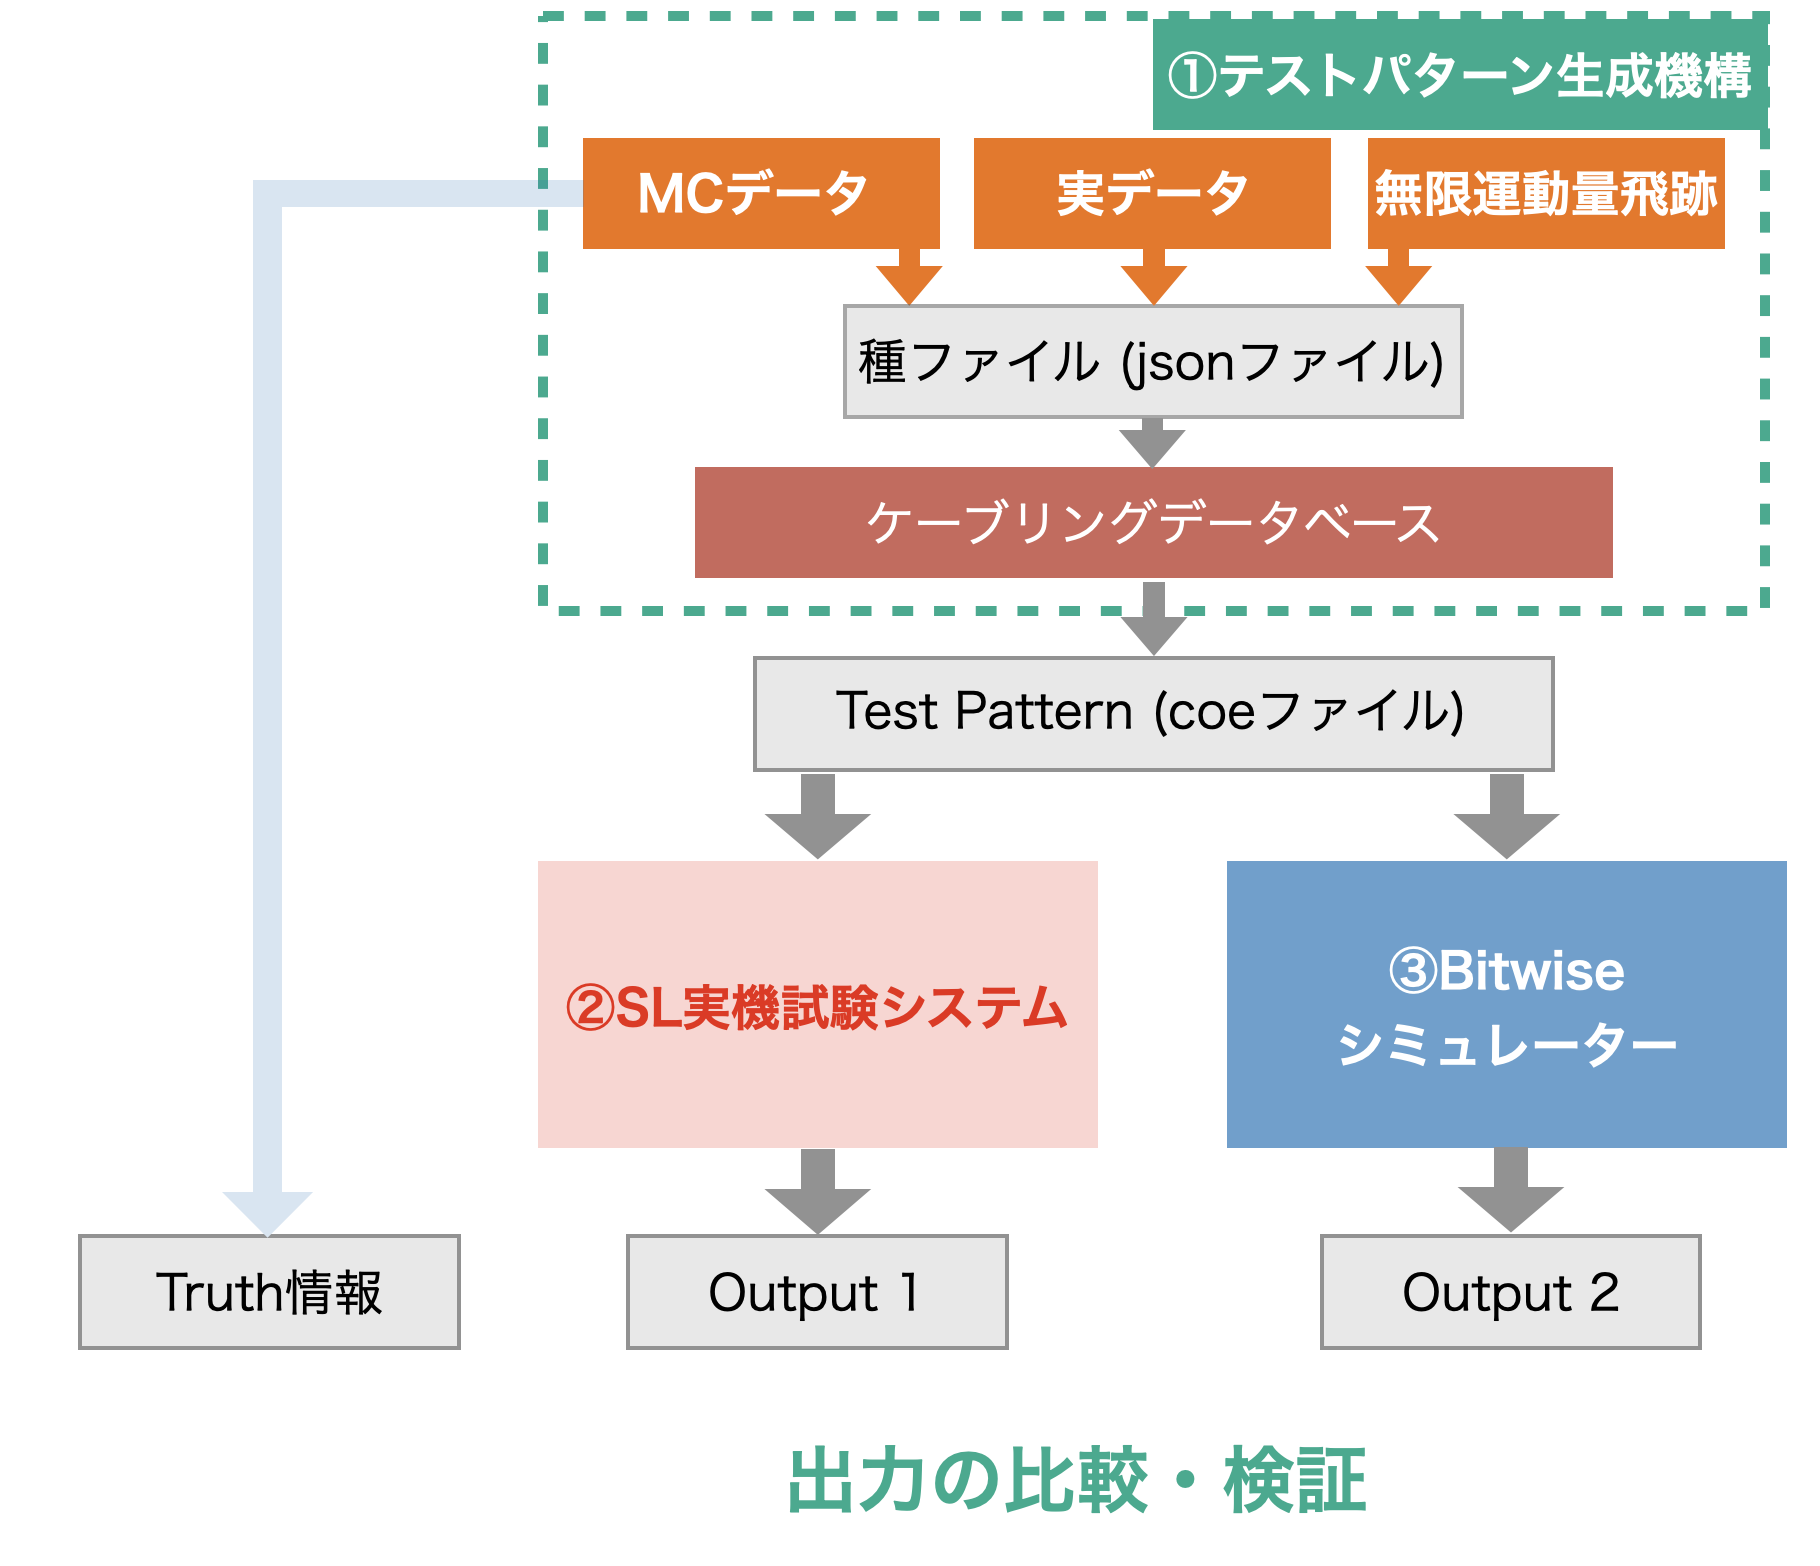
\includegraphics[width=16cm]{fig/Test/Test_system.png}
\caption[実機試験システムの概要]{実機試験システムの概要。テストパターン生成機構、SL実機試験システム。Bitwiseシミュレーターで構成される。テストパターン生成機構はMCデータ、実データ、無限運動量飛跡などをもとに、実機試験システムとBitwiseシミュレーターに共通するテストパターンを生成する。実機試験システムはこれを入力として、実機上で動作するトリガー回路の演算結果を出力する。Bitwiseシミュレーターもこれを入力として、トリガー演算をBitレベルで再現したソフトウェアエミュレーターの演算結果を出力とする。この2つの出力を相互に比較・検証することで、盤石に試験を進める。}
\label{Test_system}
\end{figure}

\paragraph{テストパターン生成システム}  
\par
\ref{chap_TGC}節で述べたようにSLは、1枚のPS boardから2本の光ファイバーを通じて128 bit $\times$ 2 ファイバーのヒット信号を受け取る。1枚のSLは合計 31枚のPS boardと接続するため、イベントごとに128 bit $\times$ 62 ファイバーのヒットビットマップがトリガーロジックに入力される。モンテカルロシミュレーションや過去のRunで取得された実データから、トリガーロジックに入力されるヒットビットマップを生成する仕掛けが、テストパターン生成システムである。

テストパターン生成システムは、元のデータセットに格納されている、TGC検出器のヒットチャンネル情報を抽出し、テストパターンの種ファイルであるjsonファイルを作成する。この際、モンテカルロデータ、実データ、toyデータなどいかなるデータセットも統一的なフォーマットでjsonファイルへ記述することで、この後の処理はその違いに関わらず進めることができる。生成されたjsonファイルはケーブリングデータベースと接続される。ケーブリングデータベースはTGC検出器からSLまでの複雑な配線情報 (ASD、PS board、SLと続く物理的なケーブルの配線に加え、各デジタル回路内の信号の並び替え情報等も含む) を一元的に管理しているデータベースである。この2つを合わせることで、任意のデータセットからSLのインプットを再現したテストパターンを生成することができる。テストパターンはSL実機、Vivado シミュレーション、後述するBitwiseシミュレーターに共通の形式で入力でいるようcoeファイル形式で出力される\footnote{テストパターンは論理回路内でBRAMに格納される。BRAMはcoeファイル形式により初期化することができ、これに合わせるように実機試験システム、Bitwiseシミュレーターを開発した。}。これにより、全く同じインプットを入力に用いた、コヒーレントな検証が可能になっている。

\paragraph{実機試験システム}  
\par
実機試験システムは生成されたテストパターンをインプットに、実際にハードウェア上でトリガー回路を動作させ、その出力を取り出すシングルボード試験システムである。その詳細は次節説明する。

\paragraph{Bitwiseシミュレーター}  
\par
BitwiseシミュレーターはSLトリガーロジックをビットレベルで再現したC++ベースのシミュレーターである。このシミュレーターはテストパターンを入力とし、LUTも実機システムと同じものを使用するため、実機システムと完全に同じコンフィギュレーションの下でシミュレーションを実行することができる。そのため、実機システムとの比較・検証用に極めて有用である。また、各モジュールのロジックや入出力がファームウェアと完全に一致するよう設計されているため、途中出力同士の比較や、実機で出力できない内部の信号線の調査にも利用できる。これにより、論理回路の精密な分析と調査が可能になる。\footnote{ソフトウェアシミュレーターは実現しているロジックはファームウェアと完全に等価であるが、入力データやLUTは実機システムとは異なるため、最終的な動作確認には不向きである。また内部でビットレベルの演算を行なっている訳ではないので、途中出力をファームウェアと比較することもできない。}

\section{実機試験システムの開発}
\subsection*{ファームウェアの概要}
本節では、トリガー回路の試験用に開発したシングルボード試験システムについて説明する。
図\ref{TestSystem_Overview}に実装したトリガーロジック試験システムの全体像を示す。試験システムのコントロールおよびデータ読み出しはMPSoC上のLinuxを起点に行う。本システムではSL単体での試験を実現するため、SL上の水晶発振器で生成した40.079 MHzクロックをLHC陽子バンチ交差クロックの代わりに基準クロックとして扱う。FELIXから配られるTest Pulse Trigger (TPT)やL0AなどのTTC信号もSL内部のTTC emulatorで擬似的に生成し、各モジュールに分配する。

\begin{figure} 
\centering
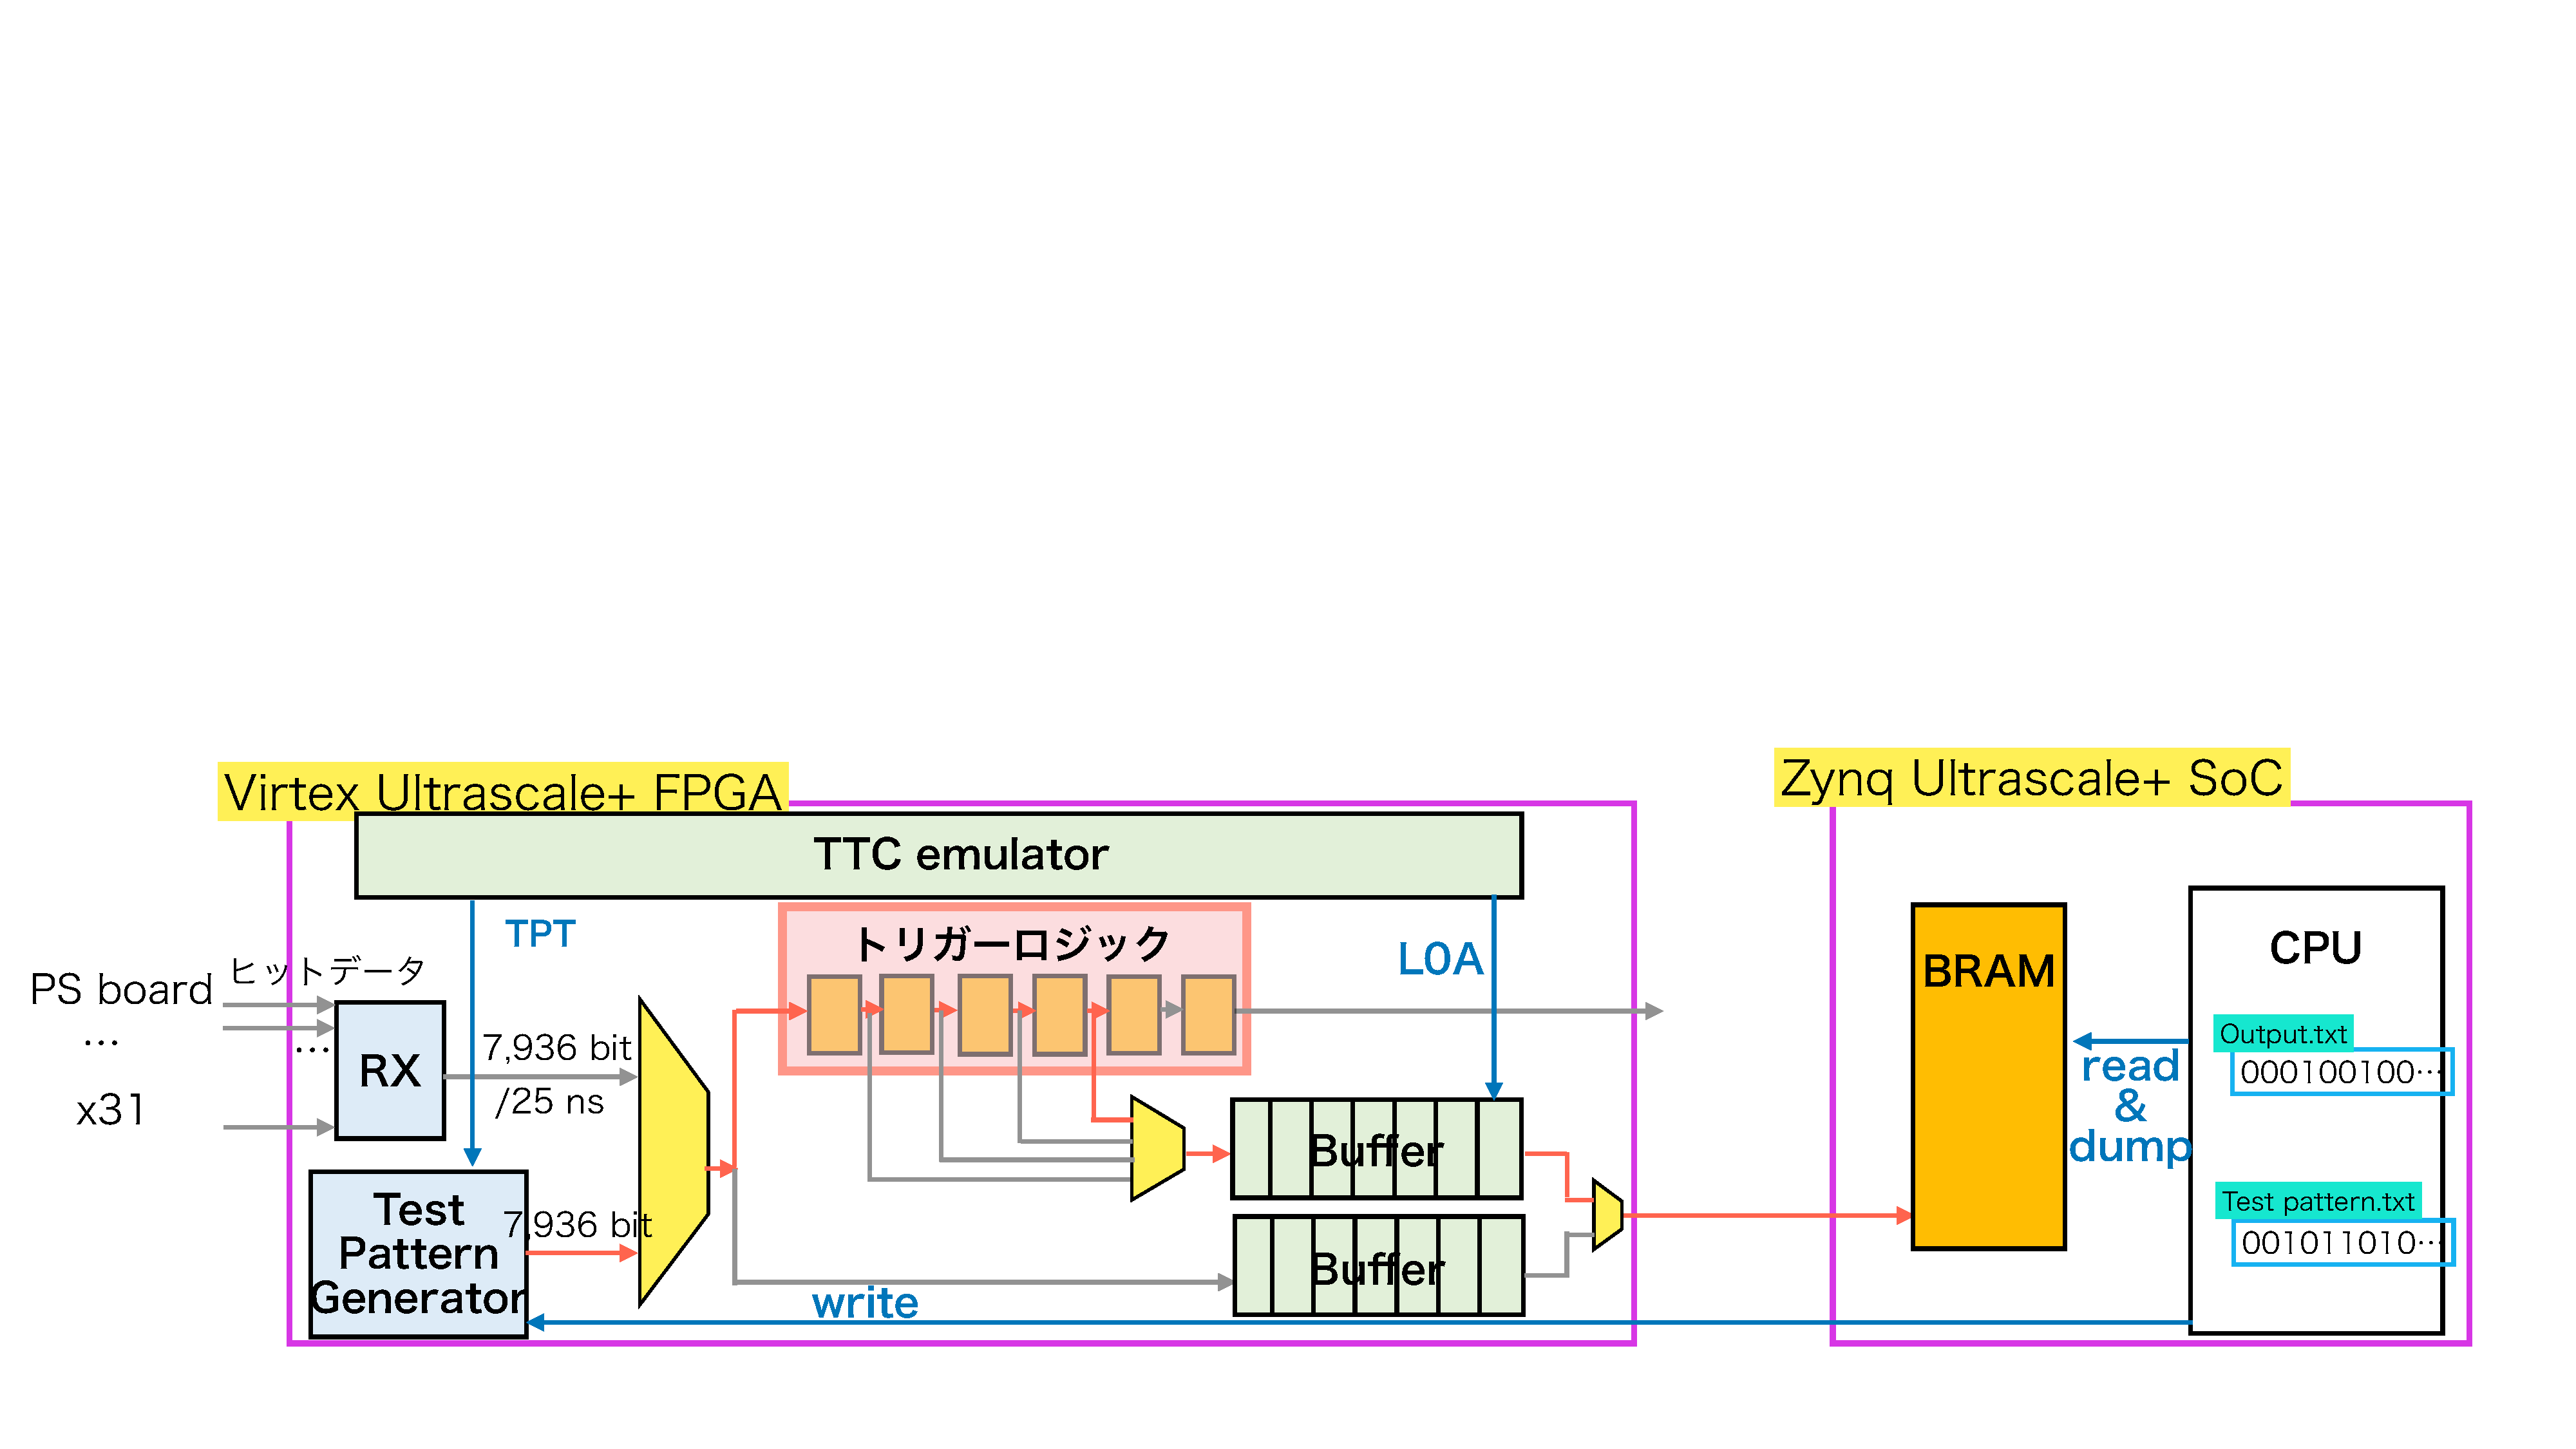
\includegraphics[width=16cm]{fig/Test/TestSystem_overview.pdf}
\caption[トリガー試験ファームウェアの概要]{トリガー試験ファームウェアの概要。MPSoC上のCPU領域に起動したLinuxを起点に、試験システムのコントロール、データ読み出しを行う。システムはSL上の水晶発振器で生成した40.079 MHzクロックをLHC陽子バンチ交差クロックの代わりに利用する。FELIXから分配されるTPT、L0A、BCRなどのTTC信号はSL内部のTTC emulatorで生成する。トリガーロジックへのヒットビットマップの入力はTest Pattern Generatorから行う。トリガーロジックの出力は読み出し回路を通じてMPSoC上のBRAMにダンプし、それをLinuxから読み出すことでトリガー演算結果を取得する。}
\label{TestSystem_Overview}
\end{figure}

PS boardから受信するヒット信号をエミュレートしたテストパターンは、Test Pattern Generator内のBRAMに格納される。Test Pattern GeneratorはTTC emulatorからTest Pulse Trigger (TPT) 信号を受信すると、1イベント分のヒットビットマップをトリガー回路に投入する。Trigger Logicからの出力はLHCバンチ交差クロックに同期してL0 Bufferにダンプされ、読み出し回路を経てMPSoC上のLinuxから読み出される。トリガー回路は固定レイテンシーで動作するため、TTC emulatorはTPTから決まったクロックチック後にL0Aを出すことで、テストパターンに該当するトリガー出力を読み出すことができる。以下に各モジュールの概要を説明する。

\paragraph{Test Pattern Generator}  
\par
Test Pattern Generator は幅 128 bit、深さ 64 列 のBRAMにテストパターンを保存し、TTC emulatorからTPTが供給されたタイミングで擬似データをトリガー回路に投入する。1つのBRAMがPS board 1リンク分の信号を保存する。全31 PS board $\times$ 2リンクの信号をエミュレートするために、Test Pattern Generatorには合計62個のBRAMが並列に配置されている。トリガーロジックの入力にPS boardから受信したヒットデータを用いるか、Test patternを用いるかはスイッチで切り替えられるようになっている。

BRAMにはcoe形式のファイルを利用して初期値を設定できるほか、MPSoCから何度でもテストパターンを上書きすることができる。そのため、BRAMの深さに制限されることなく任意のイベント数で試験することができる。


\paragraph{トリガーロジック中間状態の読み出し回路}  
\par
トリガー回路の出力は読み出し用のフォーマットに成形され、トリガー読み出し回路へ渡される。今回の試験では各モジュールの動作を詳細に調査するため、モジュール間で受け渡される全てのビットマップを読み出せるようフォーマットを定義している。例としてWire Strip Coincidenceの読み出しデータを説明する。
Wire Strip Coincidenceは8 Unit regionから1 つののミューオン候補を、32 Unit regionから4 つののミューオン候補をそれぞれ出力し、最大180個のミューオン飛跡候補をInner Coincidenceに送る。読み出し回路はこの最大180個のミューオン候補を並列に読み出せるよう設計しており、各領域ごとに表\ref{tab:WS_format}のフォーマットに飛跡情報を成形する。各モジュールの出力フォーマットは最上位1 bitがvalid信号として定義され、後段の読み出し回路ではvalid信号が立てられたイベントのみを選択的に読み出す。これにより、効率的にデータ量を削減している。

\begin{table}[]
    \centering
    \caption[Wire Strip Coincidenceの読み出しフォーマット]{Wire Strip Coincidenceの読み出しフォーマット。}
    \label{tab:WS_format}
    \begin{tabular}{|c|c|}
    \hline
    \# of bits & Name                                                                                        \\ \hline\hline
    1          & The flag indicates that the region has received at least one wire segment and strip segment \\ \hline
    4          & $p_{\mathrm{T}}$ threshold reconstructed using Coincidence                                  \\ \hline
    3          & Reserved                                                                                    \\ \hline
    7          & $\Delta\theta$ from Wire Segment Reconstruction                                             \\ \hline
    2          & Number of stations with the hits used for wire segment                                      \\ \hline
    4          & $\Delta\phi$ from Strip Segment Reconstruction                                              \\ \hline
    2          & Number of stations with the hits used for strip segment                                     \\ \hline
    1          & Reserved                                                                                    \\ \hline
    \end{tabular}
\end{table}


それぞれのトリガーモジュールから読み出すデータの出力ビット幅を表\ref{tab:output_width}に示す。後述するトリガー読み出し回路において、数千ビットの信号を一度に処理しようとすると、タイミング制約を満たしてロジックを配置することが難しくなる。そこでバス幅が大きい信号線はいくつかの並列な処理レーンに分割する。

\begin{table}[]
    \centering
    \caption[各モジュールの出力ビット幅]{各モジュールの出力ビット幅。}
    \label{tab:output_width}    
    \begin{tabular}{|c|c|c|c|}
    \hline
    トリガーロジック                                      & SLR & 出力ビット幅 (bits) & レーン数 \\ \hline\hline
    \multirow{3}{*}{Channel Mappin}               & 0   & 2732          & 4    \\ \cline{2-4} 
                                                  & 2   & 2732          & 4    \\ \cline{2-4} 
                                                  & 3   & 1000          & 2    \\ \hline
    \multirow{3}{*}{Wire Station Coincidence}     & 0   & 1768          & 3    \\ \cline{2-4} 
                                                  & 2   & 1768          & 3    \\ \cline{2-4} 
                                                  & 3   & 804           & 3    \\ \hline
    \multirow{3}{*}{Strip Station Coincidence}    & 0   & 1890          & 3    \\ \cline{2-4} 
                                                  & 2   & 1890          & 3    \\ \cline{2-4} 
                                                  & 3   & 378           & 3    \\ \hline
    \multirow{3}{*}{Wire Segment Reconstruction}  & 0   & 3404          & 5    \\ \cline{2-4} 
                                                  & 2   & 3404          & 5    \\ \cline{2-4} 
                                                  & 3   & 1472          & 2    \\ \hline
    \multirow{3}{*}{Strip Segment Reconstruction} & 0   & 360           & 1    \\ \cline{2-4} 
                                                  & 2   & 360           & 1    \\ \cline{2-4} 
                                                  & 3   & 72            & 1    \\ \hline
    \multirow{3}{*}{Wire Strip Coincidence}       & 0   & 1776          & 3    \\ \cline{2-4} 
                                                  & 2   & 1776          & 3    \\ \cline{2-4} 
                                                  & 3   & 768           & 1    \\ \hline
    \end{tabular}
\end{table}

また、全てのトリガーロジックの読み出し回路を同時に実装するのはリソースの観点で不可能である。トリガーモジュールごとに異なるファームウェアを用意して試験を行うことにする。実験本番で用いるファームウェアでは、各トリガーロジックからの出力から必要最低限な情報を抜き出すことで、全てのトリガーモジュールの出力を同時にモニターする予定である。

\paragraph{トリガー読み出し回路}  
\par
トリガー読み出し回路はトリガーモジュールの出力をMPSoCから読み出すための仕掛けである。図\ref{Readout_Circuite}に読み出し回路の概要を示す。以下に各モジュールの役割を説明する。

\begin{figure} 
\centering
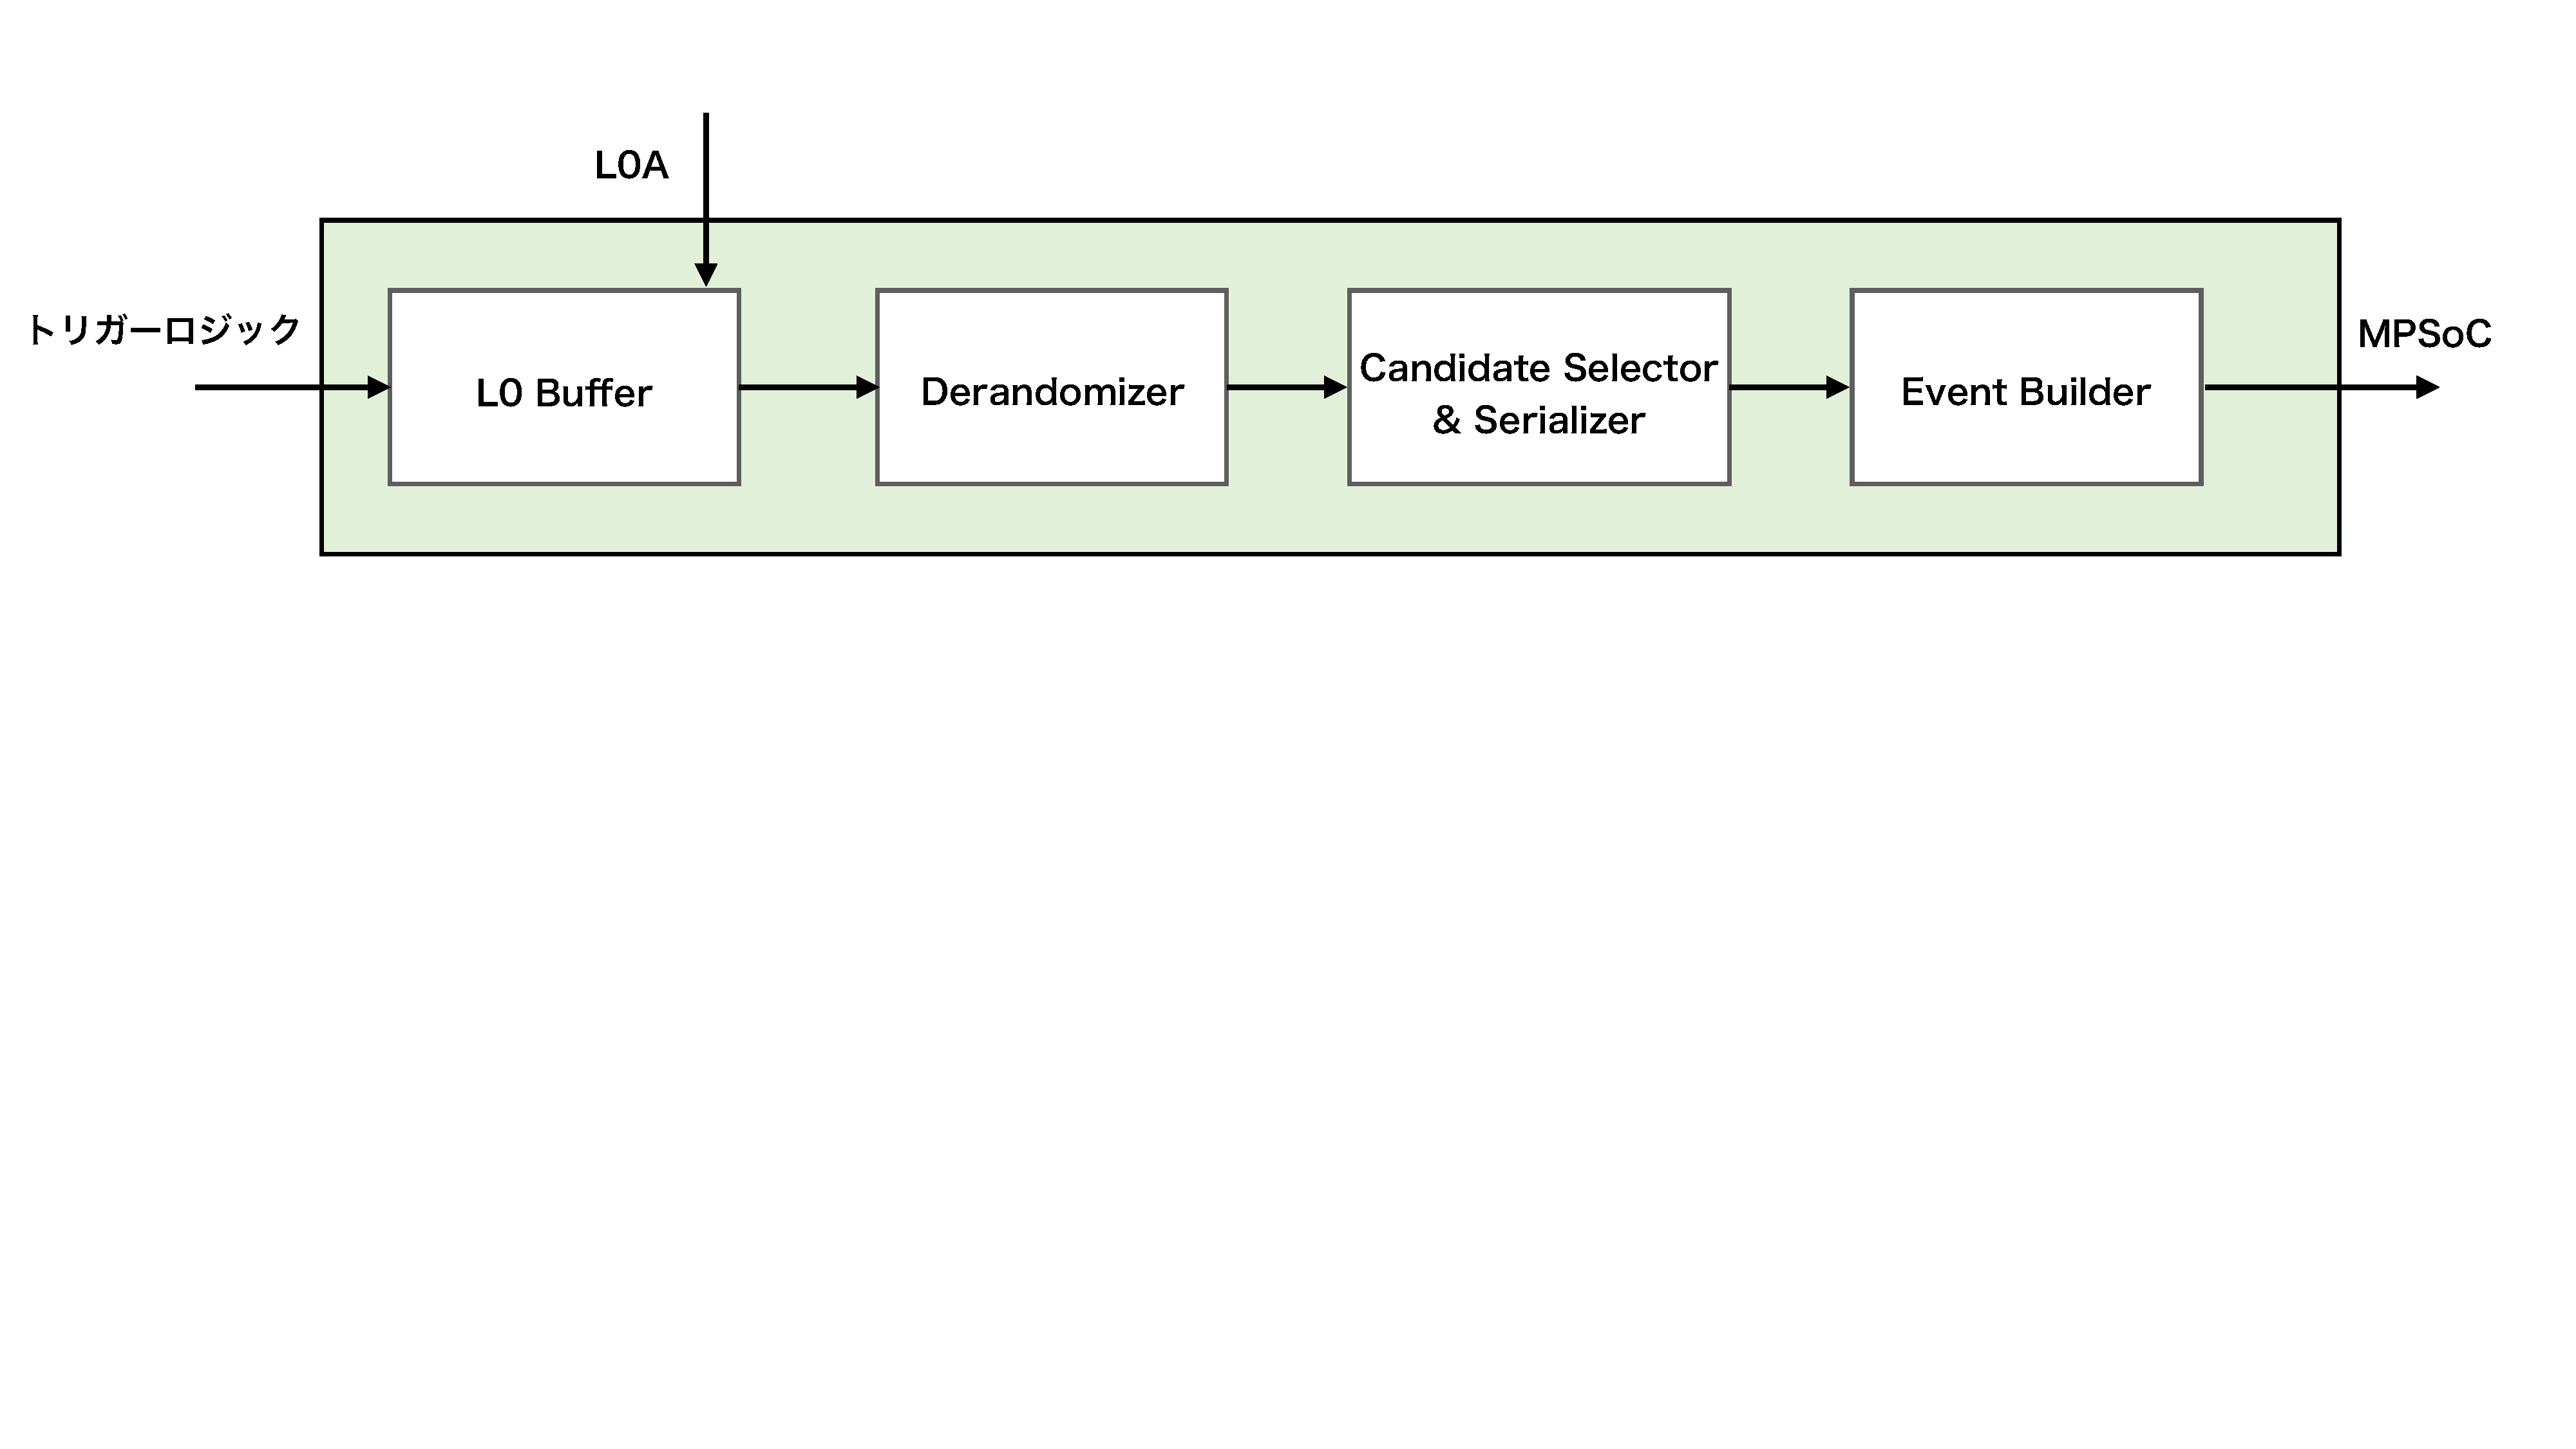
\includegraphics[width=16cm]{fig/Test/Readout_Circuite.pdf}
\caption[トリガー読み出し回路の概要]{トリガー読み出し回路の概要。トリガーロジックからの出力はL0 Bufferに格納され、L0Aが出されたイベントのみDerandomizerに送信される。トリガーモジュールからの出力は、すべてのユニットからの出力を並列に並べてあるが、Candidate Selectorはこの中から飛跡を再構成できたユニットからの出力のみを抜き出して、Event Builderに送信する。Event Builderでは複数のモジュールからの出力を1つのパケットにまとめて、MPSoCへと送る。}
\label{Readout_Circuite}
\end{figure}

\begin{itemize}
    \item L0 Buffer  
    \par
    トリガーロジックでフォーマットされたデータはL0 Bufferにダンプされる。L0 Bufferは入力ビットマップと同じ幅をもつ深さ512 列のBRAMあり、TTC emulatorからL0Aが出されるまでのバッファリングを行う。トリガーロジックには40 MHz、160 MHz、240 MHzで駆動するものが存在するが、いずれのモジュールでも1つの陽子バンチ衝突由来の出力は25 nsごとに横並びに揃えられ、40 MHzのLHC クロックで動作する書き込みポインタに従って、L0 Bufferに格納される。一方、読み出しは240 MHzで行われ、読み出されたデータはDerandomizerに送られる。

    \item Derandomizer  
    \par
    Derandomizerは入力ビットマップと同じbit幅をもつ深さ 512 列 のFIFOで、後段で行われる圧縮およびシリアル化の処理待ち用バッファーとして動作する。後段のCandidate Selector から読み出し命令を受け取るたびに、FIFOの先頭のイベントを出力する。

    \item Candidate Selector \& Serializer  
    \par
    Candidate Selectorは各トリガーモジュールのすべてのユニットから出力される飛跡候補の中から、ミューオン候補を再構成できたユニットの出力のみを選択して後段に送る。これにより大幅なデータ削減が達成される。選択された飛跡情報には、どのサブユニットからの出力かを示す6 bitの識別IDと2bit のbunch tagが付与され、32 bit幅のワードとして後段のSerializerに送信される。
    Serializerは32 bit幅のワードをクロックチックごとに1ワードずつ処理し、あるL0Aに対応する1イベント分のパケットをまとめて、後段のEvent Builderに渡す。図\ref{tab:packet_format}にパケットのフォーマットを示す。パケットにはイベント境界を示すための特別なワード Start of Event (SOE)、End Of Event (EOE) が挿入される。

\begin{itembox}{後で直すところ}
    表はみだし問題
\end{itembox}

    \begin{table}
        \centering
        \caption[パケットのフォーマット]{SerializerからEvent Builderに送られるパケットのフォーマット}
        \label{tab:packet_format}
        \footnotesize
        \begin{tabular}{|c|cccccccccccccccccccccccccccccccc|}
        \hline
                & \multicolumn{1}{c|}{31} & \multicolumn{1}{c|}{30} & \multicolumn{1}{c|}{29} & \multicolumn{1}{c|}{28} & \multicolumn{1}{c|}{27} & \multicolumn{1}{c|}{26} & \multicolumn{1}{c|}{25} & \multicolumn{1}{c|}{24} & \multicolumn{1}{c|}{23} & \multicolumn{1}{c|}{22} & \multicolumn{1}{c|}{21} & \multicolumn{1}{c|}{20} & \multicolumn{1}{c|}{19} & \multicolumn{1}{c|}{18} & \multicolumn{1}{c|}{17} & \multicolumn{1}{c|}{16} & \multicolumn{1}{c|}{15} & \multicolumn{1}{c|}{14} & \multicolumn{1}{c|}{13} & \multicolumn{1}{c|}{12} & \multicolumn{1}{c|}{11} & \multicolumn{1}{c|}{10} & \multicolumn{1}{c|}{9} & \multicolumn{1}{c|}{8} & \multicolumn{1}{c|}{7} & \multicolumn{1}{c|}{6} & \multicolumn{1}{c|}{5} & \multicolumn{1}{c|}{4} & \multicolumn{1}{c|}{3} & \multicolumn{1}{c|}{2} & \multicolumn{1}{c|}{1} & 0 \\ \hline
        SOE       & \multicolumn{5}{c|}{rsvd}                                                                                                       & \multicolumn{4}{c|}{data loss flag}                                                                   & \multicolumn{12}{c|}{0xB0E}                                                                                                                                                                                                                                                                                           & \multicolumn{11}{c|}{L0ID}                                                                                                                                                                                                                                   \\ \hline
        EOE       & \multicolumn{5}{c|}{rsvd}                                                                                                       & \multicolumn{4}{c|}{data loss flag}                                                                   & \multicolumn{12}{c|}{0xB0E}                                                                                                                                                                                                                                                                                           & \multicolumn{11}{c|}{L0ID}                                                                                                                                                                                                                                   \\ \hline
        data word & \multicolumn{6}{c|}{Unit address}                                                                                                                         & \multicolumn{2}{c|}{BC tag}                       & \multicolumn{24}{c|}{bitmap}                                                                                                                                                                                                                                                                                                                                                                                                                                                                                                                                                                                   \\ \hline
        buffer    & \multicolumn{12}{c|}{0xBFF}                                                                                                                                                                                                                                                                                           & \multicolumn{9}{c|}{rsvd}                                                                                                                                                                                                               & \multicolumn{11}{c|}{L0ID}                                                                                                                                                                                                                                   \\ \hline
        \end{tabular}
    \end{table}

    \item Event Builder  
    \par
    上述のCandidate Selectorまでは読み出しレーンごとに処理が行われる。Event Builderはこれらの並列なレーンの出力を直列化し、MPSoCに送信するためのフォーマットに成形する。Serializerから受信する32 bitのワードはEvent Builder内の処理待ちバッファーに格納される。Event Builderは処理待ちバッファーのデータを240 MHzのクロックチックごとに1ワードずつ図\ref{TriggerReadout_format}のフォーマットに成形する。meta switchは読み出しを行うトリガーロジックの選択状態を表す。meta dataは各トリガーロジックごとに送られ、そのトリガーロジックのラベル(data flavor)、読み出しを行うbunch tag ( previous, current, next, next to next )の選択状態を表す。
    実機試験ではこのようにFPGA内でエンコードされたデータを、ソフトウェア上で逐次的にデコードすることで、トリガーロジックからの出力を一意に再構成して、テキストファイルにダンプする。

    \begin{figure} 
    \centering
    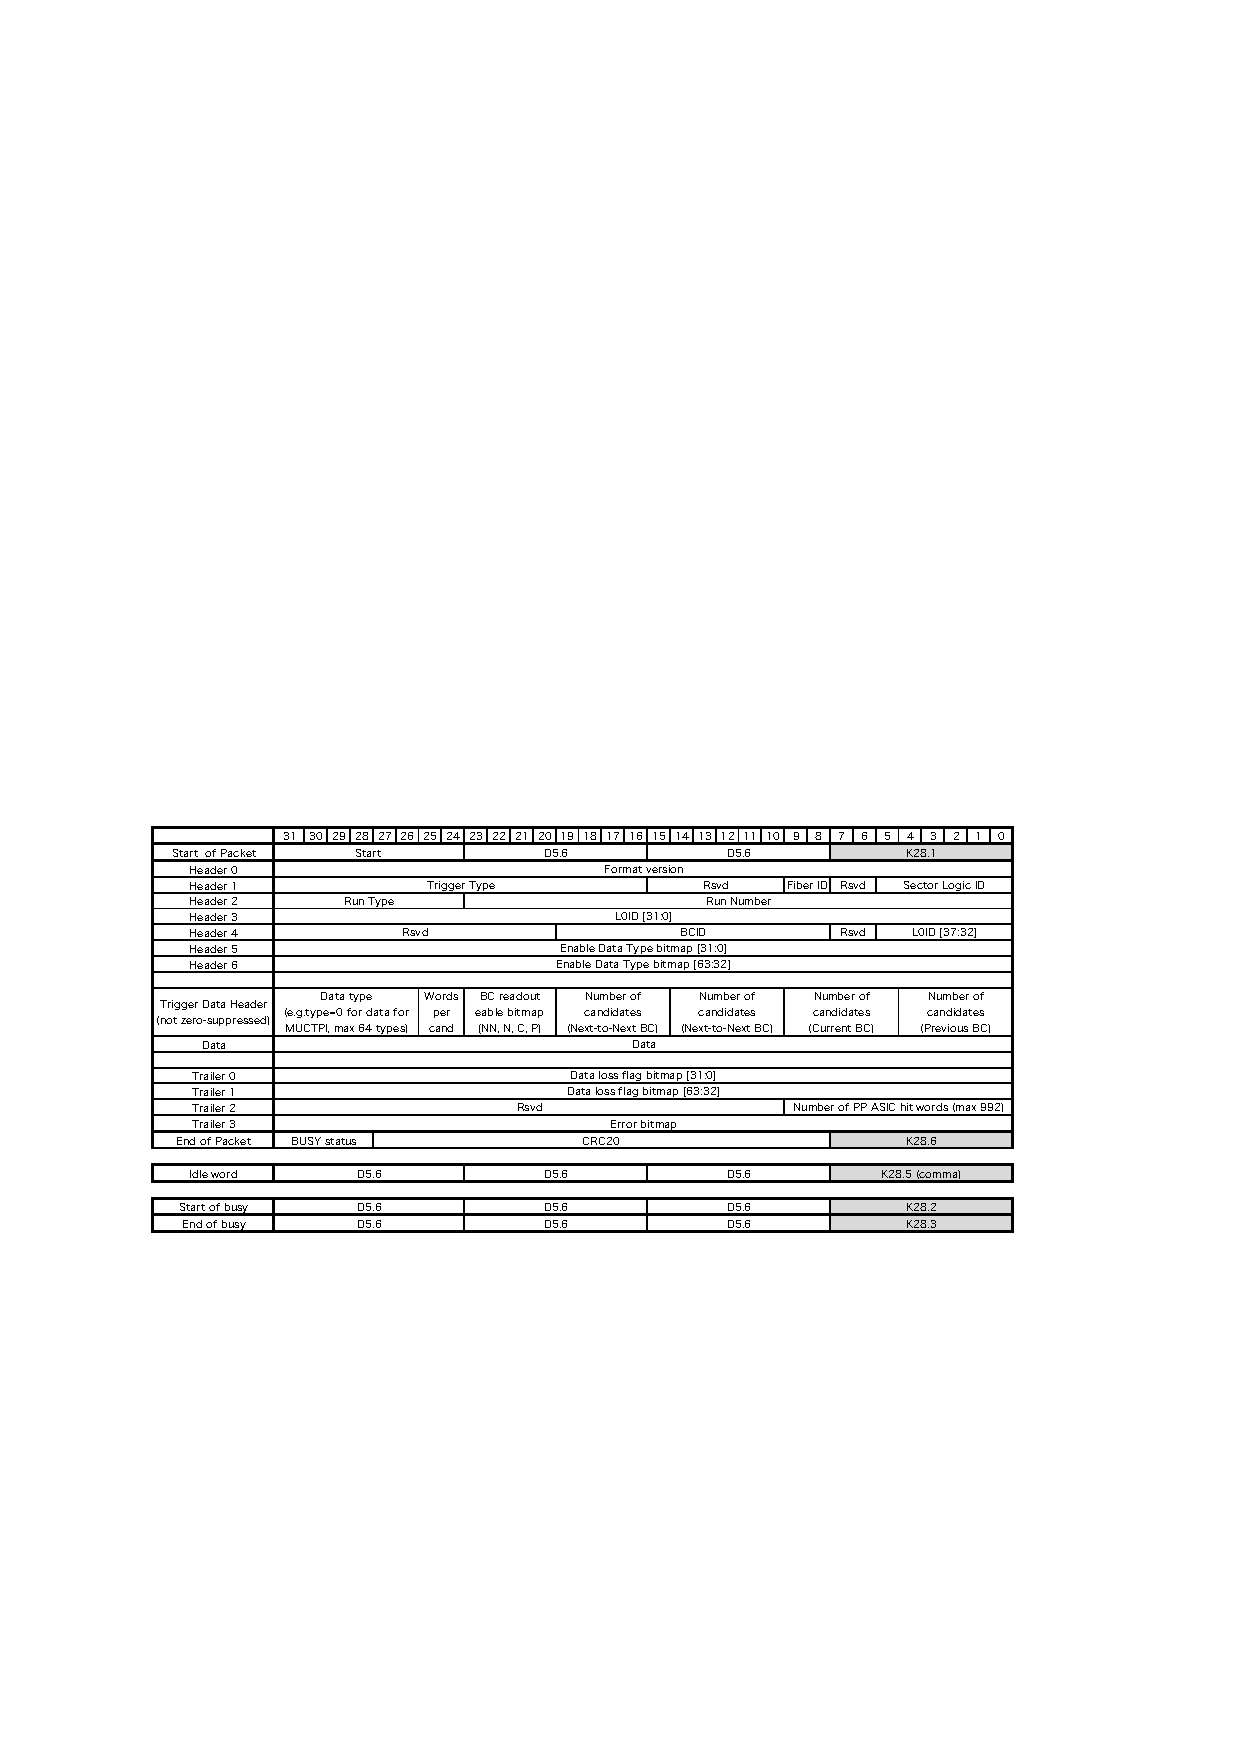
\includegraphics[width=16cm]{fig/Test/TriggerReadout_format.pdf}
    \caption[Event Builderで成形されるトリガー出力のフォーマット]{Event Builderで成形されるトリガー出力のフォーマット\cite{SLPDR}}
    \label{TriggerReadout_format}
    \end{figure}
\end{itemize}

\paragraph{SL FPGAからMPSoCへのデータ転送}  
\par
SL FPGAで成形されたデータはMPSoC PL領域内のBRAMに格納されたのち、PSから読み出される。SL FPGAからMPSoCへのデータ転送は、高速シリアル通信を利用する。図\ref{C2C}にチップ間通信の概要を示す。
\begin{figure} 
\centering
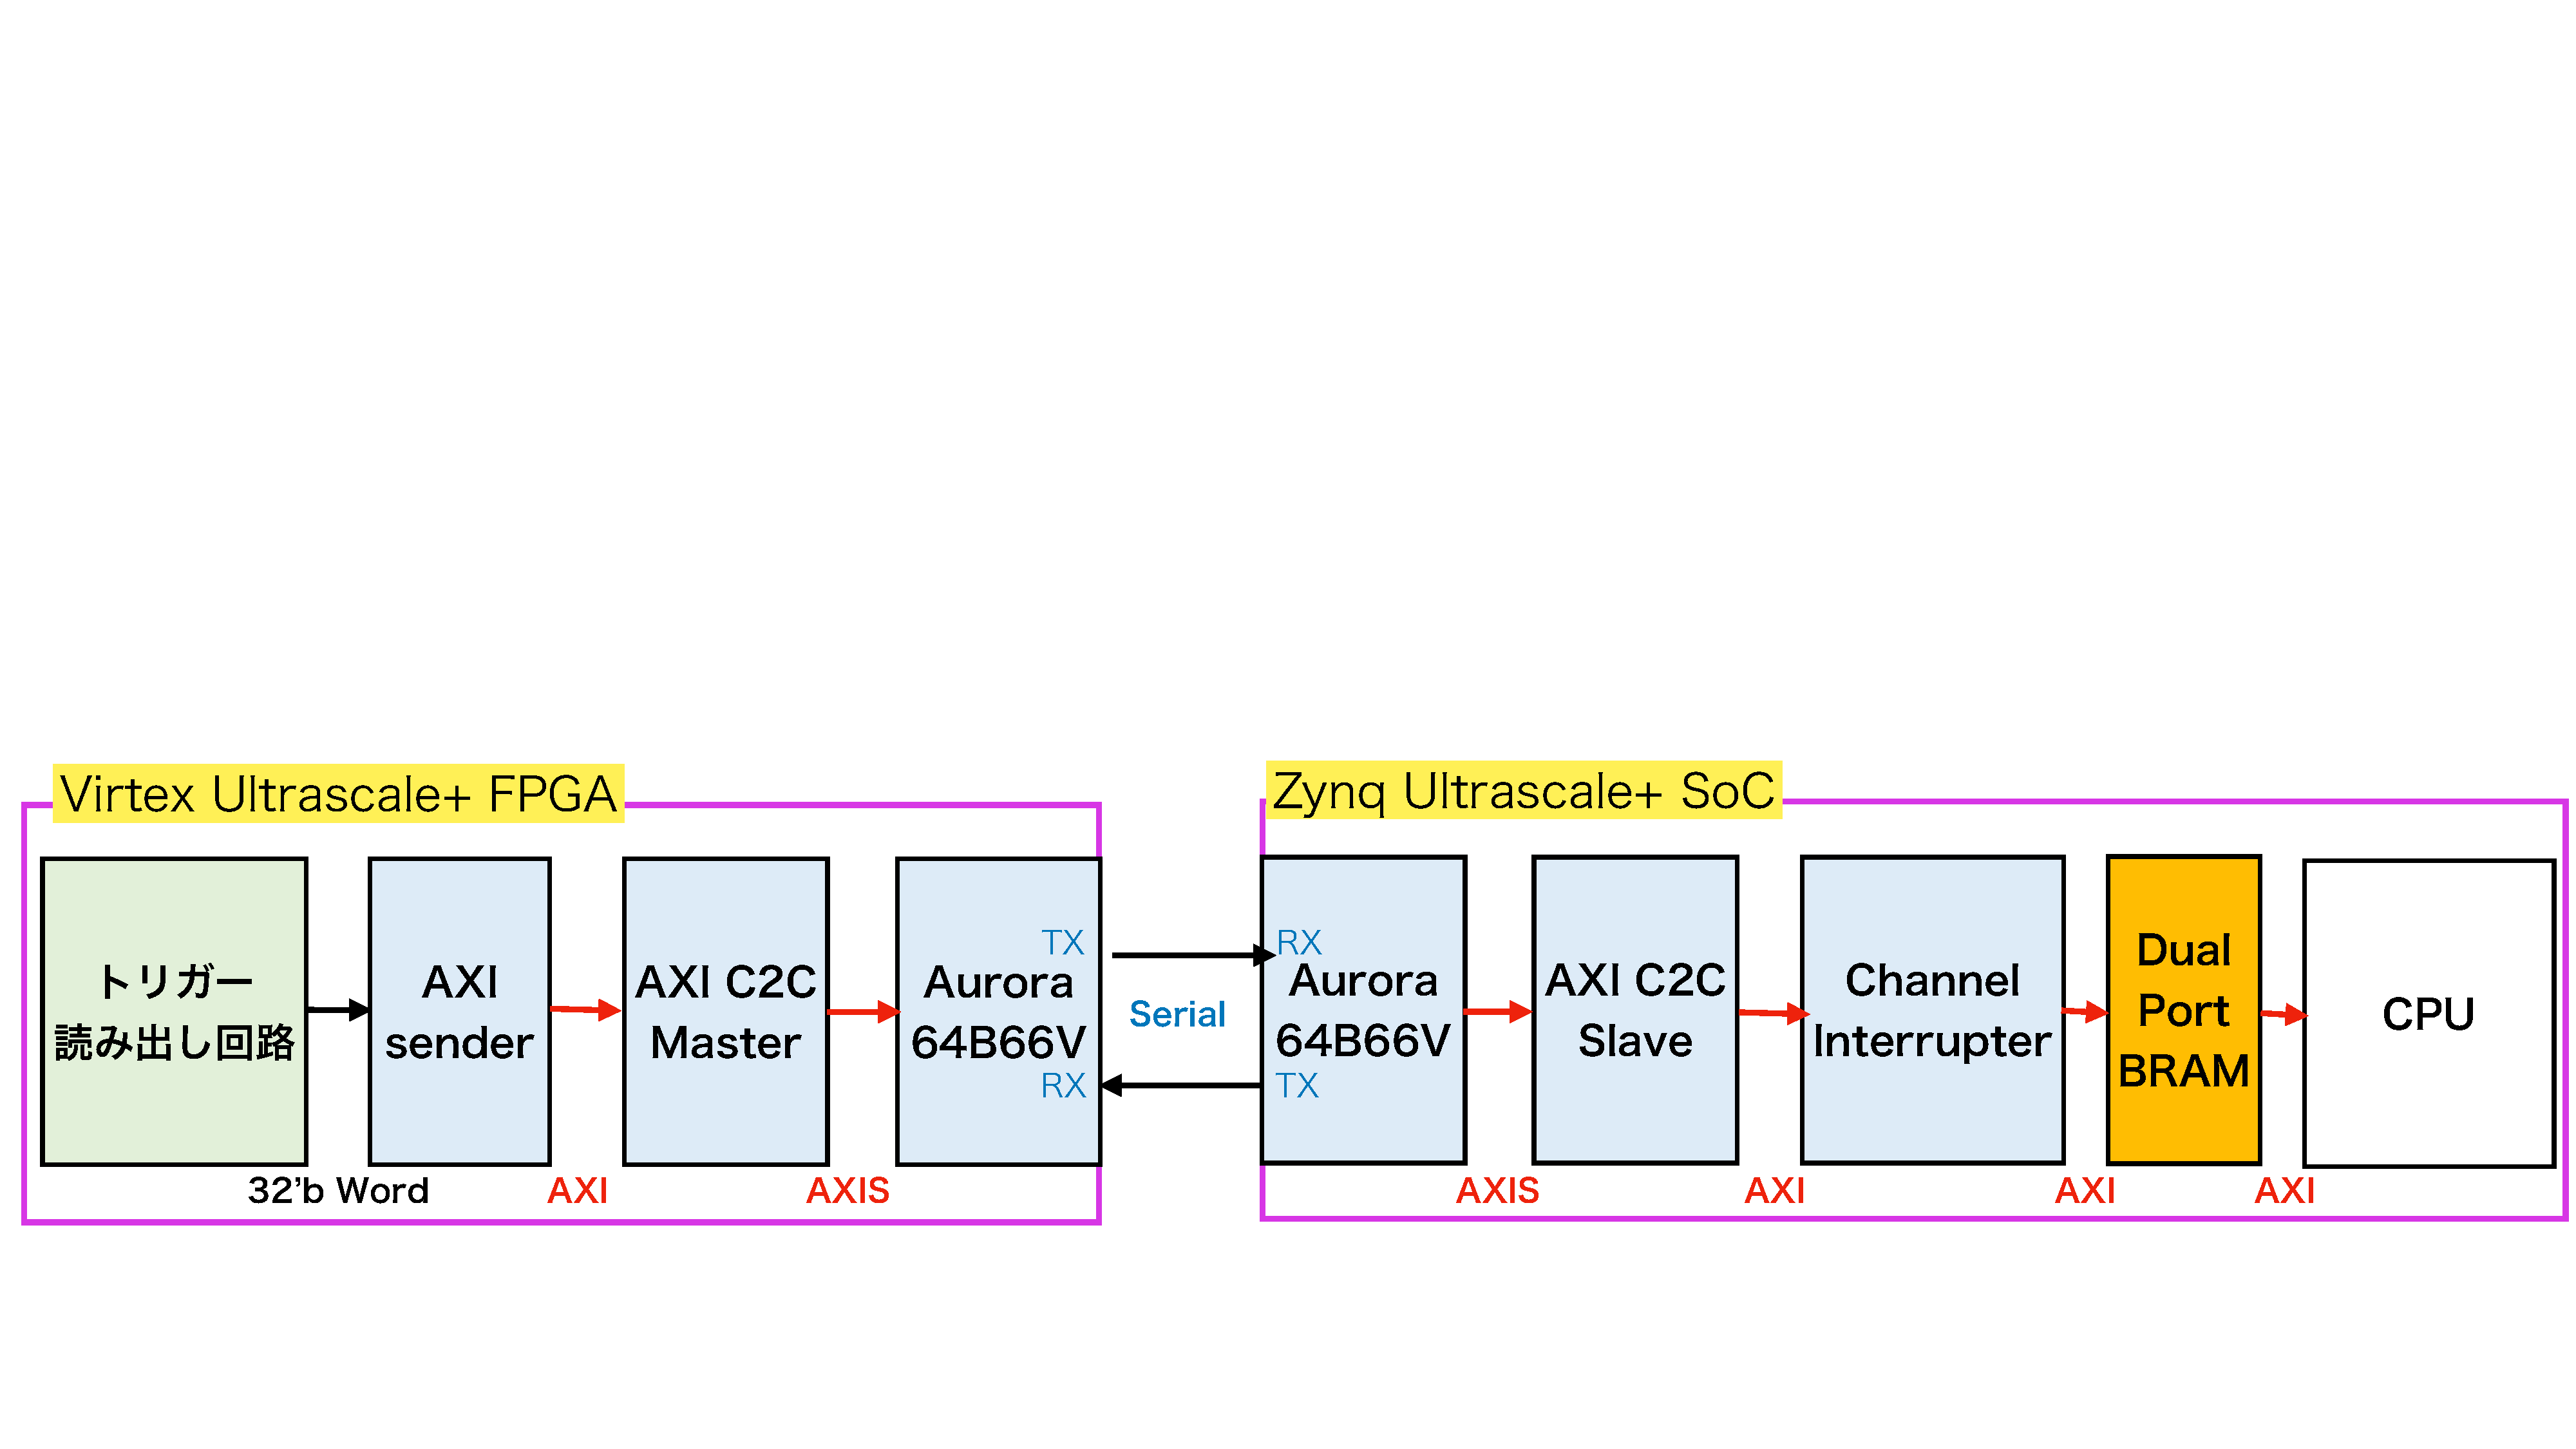
\includegraphics[width=16cm]{fig/Test/C2C.pdf}
\caption[SL FPGAからMPSoCへのチップ間通信]{SL FPGAからMPSoCへのチップ間通信。トリガー回路からの出力はAXI sender からAXI プロトコルに乗せられ、Aurora64B66Vでシリアル通信のデータにエンコードされ、MPSoCへ送られる。そのデータはMPSoCで再びAXIに載せ替えられ、BRAMにダンプされる。}
\label{C2C}
\end{figure}

Event Builderから出力される32 bit幅のワードはAXI senderに送られる。AXI senderは受信したデータをデータ幅32 bit、アドレス幅 32 bitのバス通信であるAXIプロトコルで、AXI chip2chipへ送る。AXI chip2chipはAXI形式のデータをAXI Stream 形式に変換し、Aurora 64B/66B Masterと通信する。AXI chip2chip以降のデータ転送ではAXIバーストと呼ばれる、連続したデータブロックを高速転送するための手法が採られている。AXIバーストはMasterからSlaveに送信するワード数を事前に定義 ( 本システムでは256ワード ) することで、通常のハンドシェイキングで生じるバスのアイドルタイムを最小限にする。
Aurora 64B/66B MasterはAXI Stream形式のデータをシリアル通信のデータにエンコードし、ギガビットトランシーバーを用いてチップ間通信を行う。

シリアルデータは、MPSoCのPLに実装されたAurora 64B/66B Slaveで受信され、再びAXI Stream形式にデコードされた後、AXI chip2chip でAXI 形式へと変換される。MPSoCでAXI形式に戻されたデータはChannel Interrupterを中継して、幅32bit、深さ8192 列 のdual port BRAMにダンプされる。BRAMのもう片方のポートはMPSoCのPSにAXI形式で接続されており、BRAMを介してPLからPSへのデータ送信が可能になっている。AXIバーストを利用していることで1イベント当たりのワード数は256に固定されている。そのため、BRAMに格納できるイベント数も固定であり、最大$ \,8192 / 256 = 32\,$ である。一度BRAMがfullになった場合でも、MPSoCからマニュアルでリセットをかけることで、データ取得を再開できる。

\paragraph{アプリケーション}  
\par
シングルボードのトリガー試験を行うために開発した、MPSoC上で走るアプリケーションの概要を説明する。このアプリケーションはSLのSDカード上にテキストファイルとして保存されたLUTやテストパターンをハードウェアに書き込み、トリガー演算の結果をSDカード上のテキストファイルにダンプする。
図\ref{Flowchart}にアプリケーションのフローチャートを示す。

\begin{figure} 
\centering
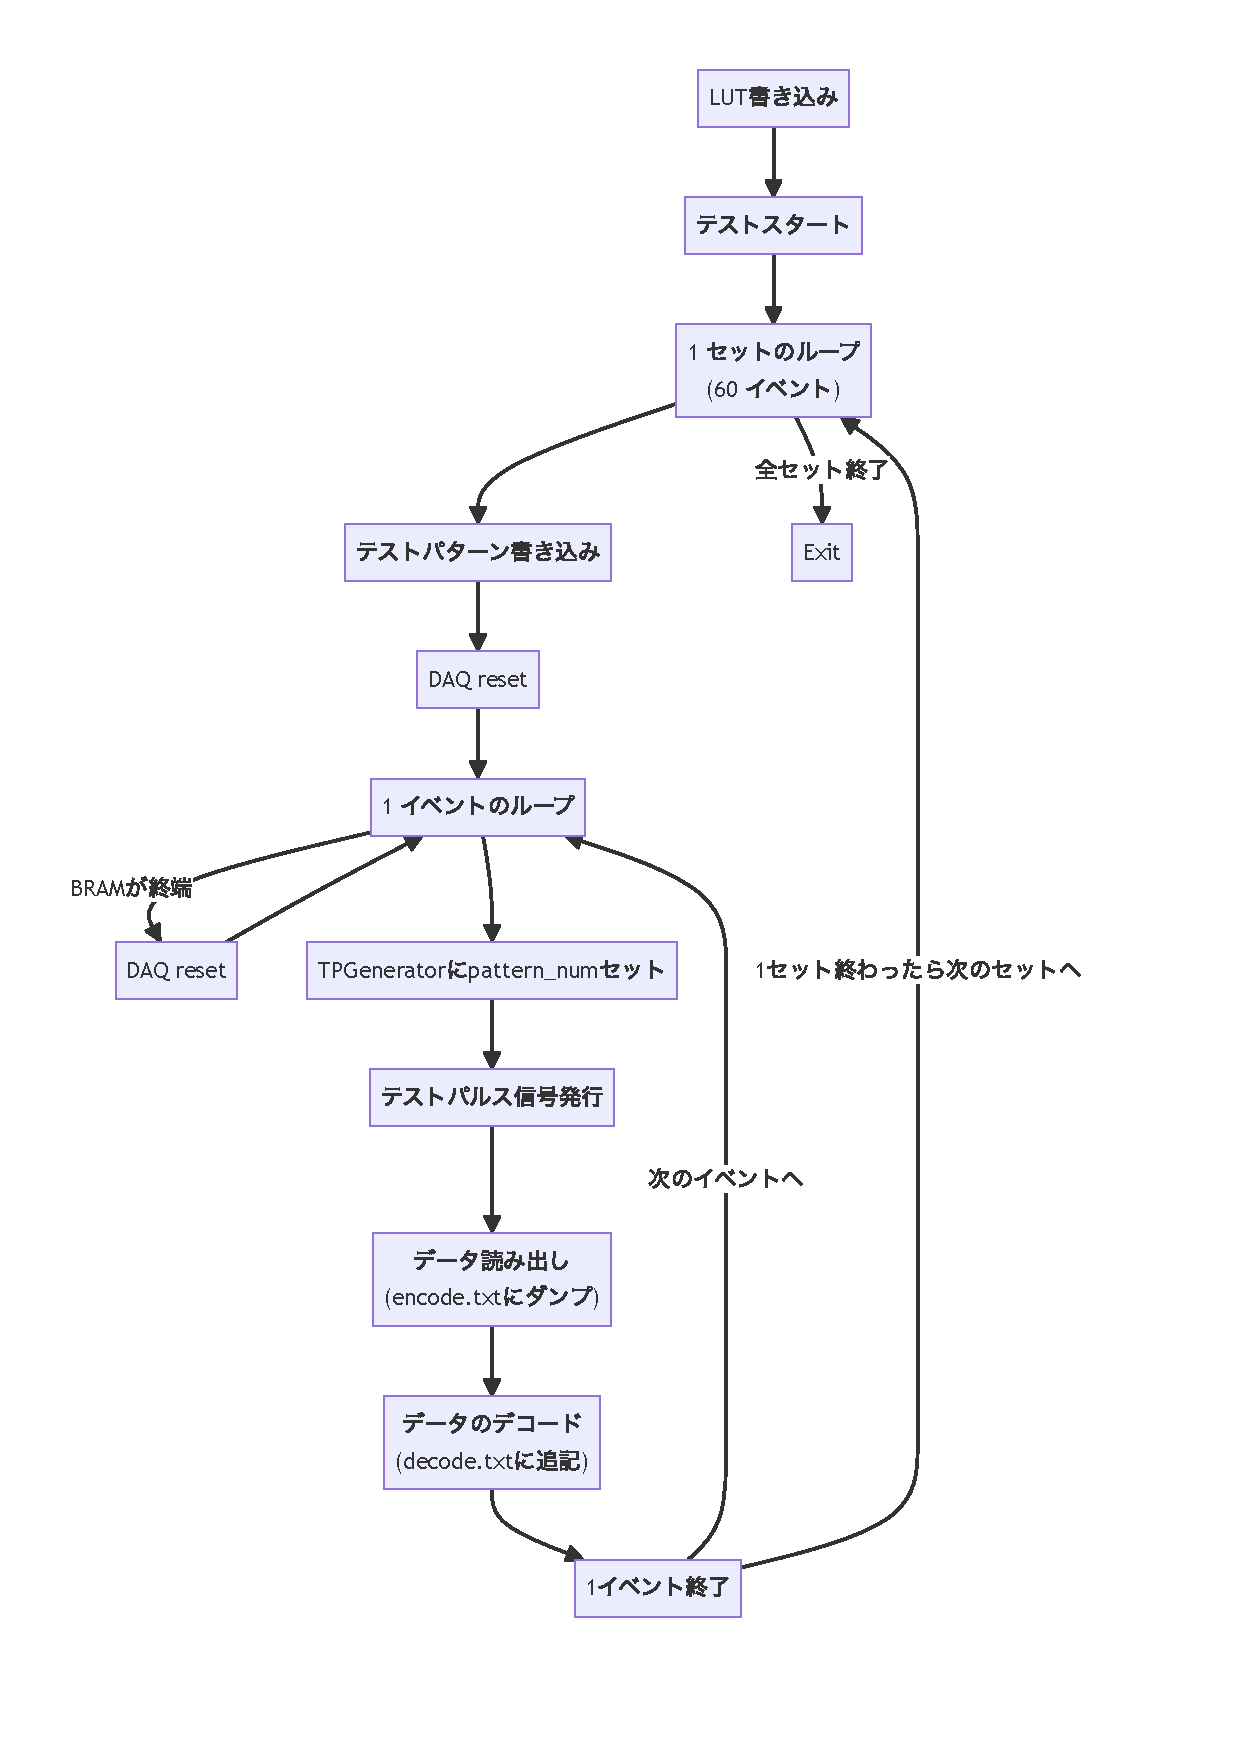
\includegraphics[width=10cm]{fig/Test/Flowchart.pdf}
\caption[アプケーションのフローチャート]{アプリケーションのフローチャート。Test Pattern GeneratorのBRAMの容量に合わせて、60イベントを1セットに試験を行う。1イベントのループでは、テストパルス信号の発行、データ読み出し、データのデコード、テキストファイルへのダンプを行う。}
\label{Flowchart}
\end{figure}

試験の最初にはLUTの書き込みを行う。LUTに利用されているURAMはファームウェア上で初期値を設定することができないため、ファームウェアを焼き直すたびに書き込み必要がある。Wire Strip CoincidenceまでのすべてのLUTを書き込むのに、概ね20分程度要する。

シミュレーションはTest Pattern Generatorに一度に書き込めるイベント数である60イベントを1セットとして、テストパターンの書き込みと60イベント分のテストを繰り返す。1イベントのループでは、最初にTest Pulse Generatorのパターンナンバーを指定し、60イベントの中から取り出すイベント番号を指定する。次にマニュアルでテストパルス信号を駆動し、トリガーロジックにデータを入力する。トリガーロジックの出力は読み出し回路を経てエンコードされたのち、MPSoC上のBRAMに格納される。格納されたデータをMPSoCのPSから取り出し、アプリケーション上でデコードする。得られたビット配列は、最終出力としてSDカード上のテキストファイルにダンプされる。イベントのループを回している過程で、MPSoCのBRAMがfullになった場合はその都度リセットをかける。

\section{無限運動量飛跡を用いた試験}
\label{sec_IMT}

本章では無限運動量飛跡と呼ばれるトイデータセットを用いて行った、トリガー回路の初等的な試験について述べる。無限運動量飛跡とは、衝突点から直線的にTGC検出器に入射するミューオンをエミュレートした試験用のイベントであり、トリガーロジックとしては100 \%再構成すべきイベントセットである。このイベントセットに対するTGC BW コインシデンスの応答を調べることで、実装したトリガーロジックが期待通り動作していることを確かめる。

以下ではまず、先行研究で開発された無限運動量飛跡生成機構について述べた後、実機試験システムを用いた試験結果について述べる。

\subsection{無限運動量生成機構}
\label{subsec_IMT_generation}

前章で述べたようにTGC検出器は位置分解能向上およびデータ量の削減を実現するため、スタッガリング構造を取っている。ステーション内の2層または3層のガスチェンバーは、各チャンネルのカバーする$\eta$領域がずれるよう設置されており、ステーション内コインシデンスにより、位置分解能を2、3倍に高めた代表点を算出する。また、M3の各代表点と同じ$\eta$に位置するM1、M2の代表点に同じ番号が割り振られるよう定義したものをスタッガードIDと呼ぶ。スタッガードIDは各ステーション内の代表点に通し番号的に振られている訳ではなく、M3の代表点を起点に、その$\eta$に一番近いチャンネルを選ぶようにして値を割り振っている。\footnote{TGC検出器が設計された当初は、各ステーションで$\eta$の位置分解能が均一になるようにワイヤーがバンドルされていたため、ステーション内で通し番号的にスタッガードIDを割り振ることができるはずだった。しかし、設置の段階でTGC検出器の設置位置がz方向にずれたため、これはできなくなった。}

% \begin{figure} 
% \centering
% 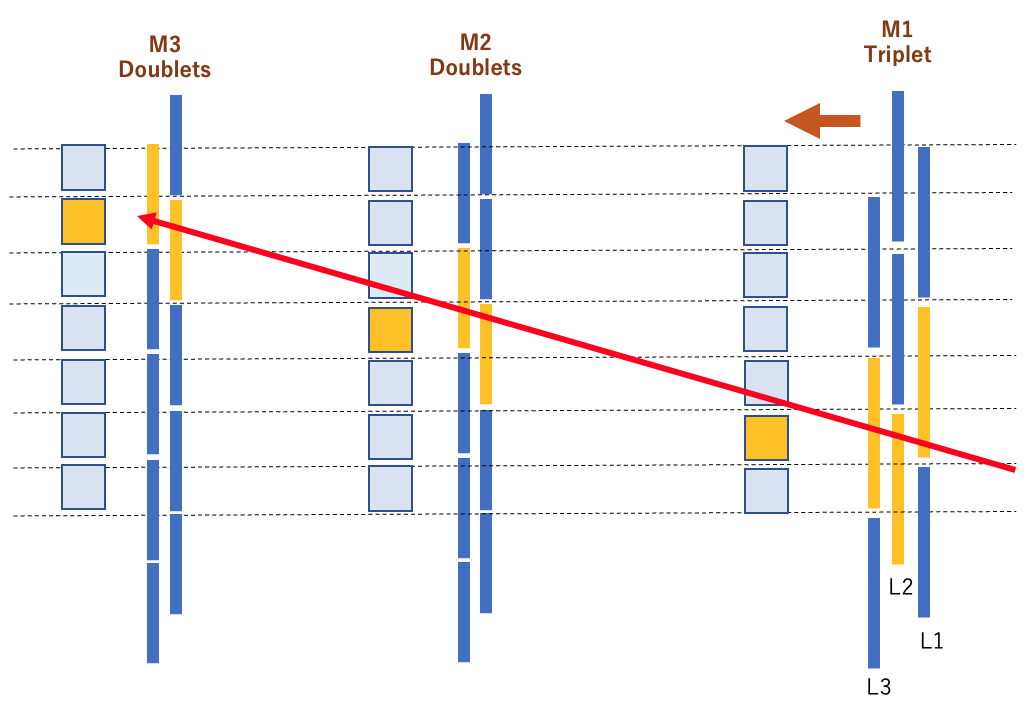
\includegraphics[width=16cm]{fig/Test/StaggerdID.png}
% \caption[スタッガードIDの概念図]{スタッガードIDの概念図}
% \label{StaggerdID}
% \end{figure}

スタッガードIDはケーブリングデータベースにより、各検出器のチャンネル番号と紐づけられている。テストパターン生成機構にはそれら活用して、任意の代表点に入射する無限運動量飛跡を作成する機構が備わっている。とある$\eta$位置に入射するミューオンをエミュレートしたテストパターンが作りたい場合、スタッガードIDを指定するだけで、それに対応する7層のヒット情報が一意に決められ、テストパターンが生成される。ストリップに対しても同様の仕掛けが作られており、$\eta$と$\phi$のスタッガードIDをそれぞれ指定することで、任意の ($\eta$、$\phi$) に入射するミューオンを模したテストパターンを作成することができる。


\subsection{無限運動量飛跡を用いたトリガーロジックの試験}
トリガーロジックおよびLUTに対する最初の試験として、図\ref{InfMomentum}に示すようにM3のWire、Stripで張られる全2次元格子点に対して無限運動量飛跡を用意した。Wire Segment Reconstruction、Strip Segment Reconstruction、Wire Strip Coincidenceのそれぞれにおいて、すべてのイベントがトリガーをパスすることを確認することで、TGCの全領域にわたってトリガーロジックが期待通りに動作していることを検証する。フォワード領域にはM3のWireの代表点が243 チャンネル、Stripの代表点が63 チャンネル存在し、合計15,309の2次元格子点が存在する。エンドキャップ領域には$\phi$0、$\phi$1 それぞれでM3のWireの代表点が 579 チャンネル、Stripの代表点が 63 チャンネル存在し、合計36,477の格子点が存在する。

\begin{figure} 
\centering
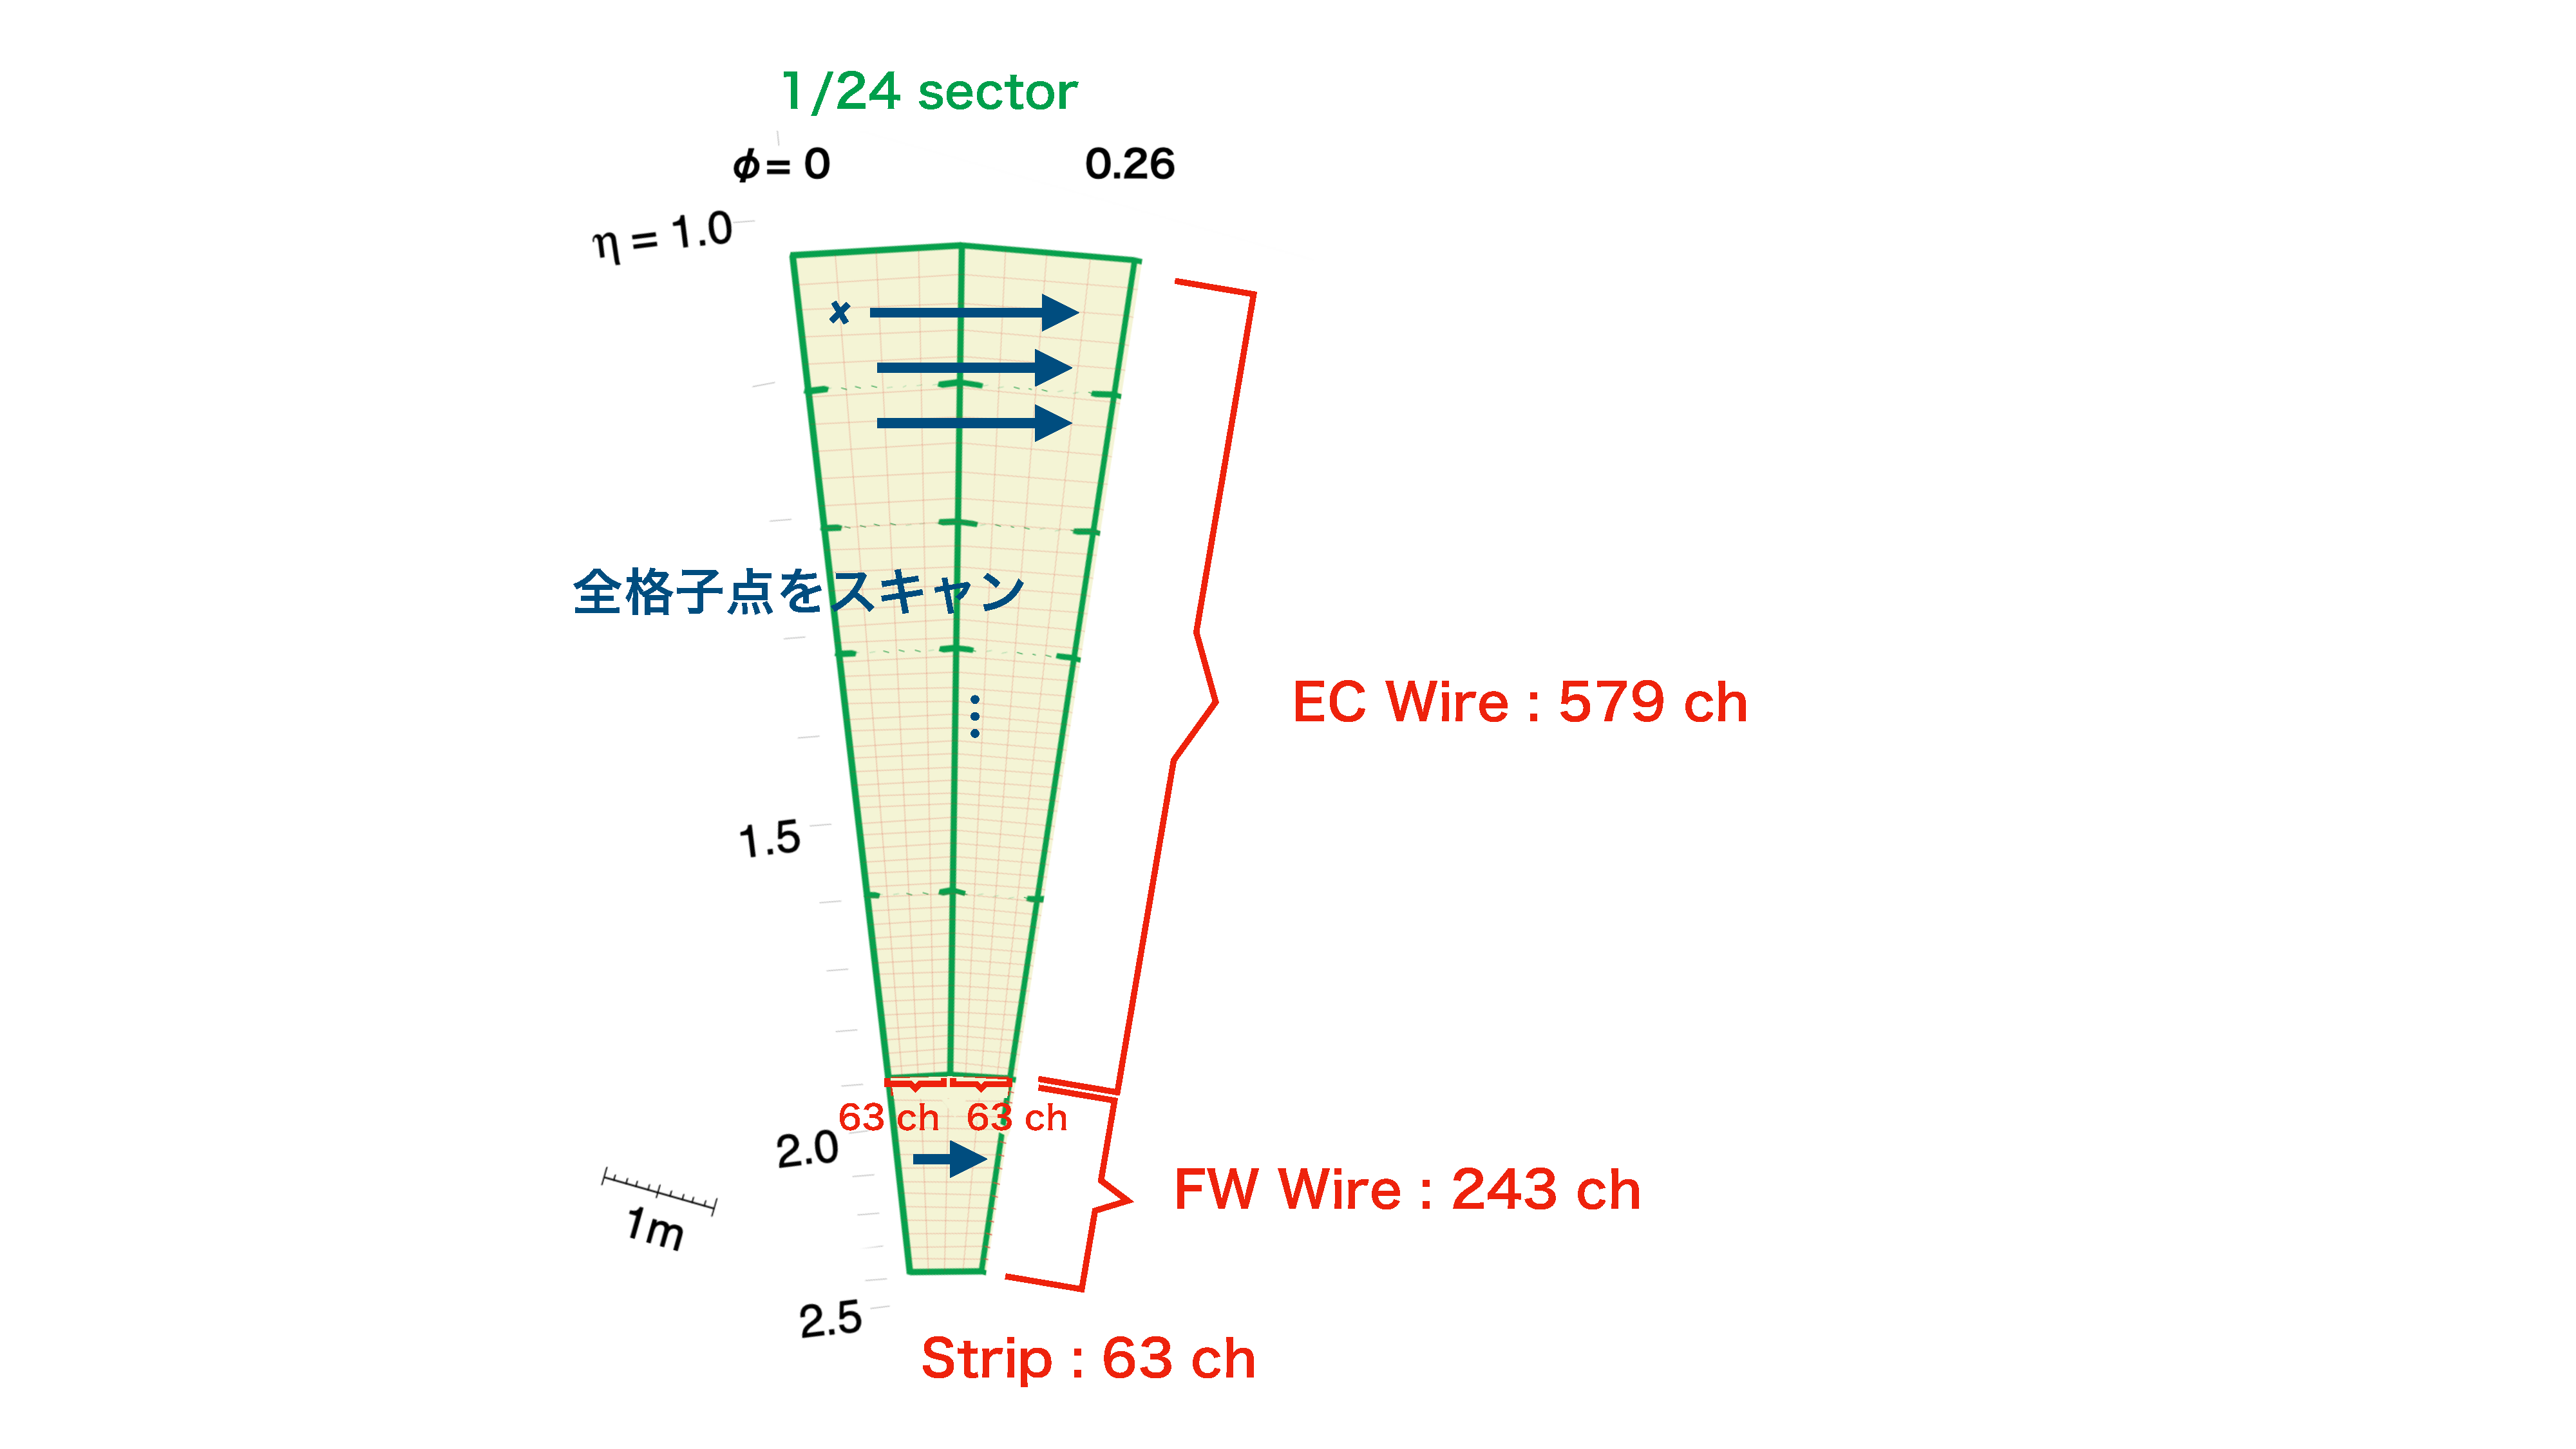
\includegraphics[width=10cm]{fig/Test/InfMomentum.pdf}
\caption[用意した無限運動量飛跡のデータセット]{用意した無限運動量飛跡のデータセット。FW、EC領域に存在する全2次元格子点に対して網羅的にテストパターンを用意。EC $\phi\,0$、$\phi\,1$領域はWireが579 ch、Stripが63 chあるため合計15,309の格子点が存在する。FW領域はWireが243 ch、Stripが63 chあるため合計36,477の格子点が存在する。}
\label{InfMomentum}
\end{figure}

図\ref{Inf_A_Strip}$\sim$図\ref{Inf_A_WS}に各モジュールごとの結果を示す。横軸にM3におけるStripのスタッガードID、縦軸にM3におけるWireのスタッガードIDをとる。各格子点をピボットとする無限運動量飛跡を実機試験システムに投入し、飛跡再構成に成功した場合はその格子点を白色、失敗した場合は黒色で塗り潰す。飛跡再構成に成功したイベントの割合を表\ref{tab:InfMomentum}にまとめる。

\begin{table}[]
    \centering
    \caption[無限運動量飛跡に対するトリガーロジックの応答]{無限運動量飛跡に対する飛跡再構成の成功率}
    \label{tab:InfMomentum}
    \begin{tabular}{|c|c|c|c|}
    \hline
        & \begin{tabular}[c]{@{}c@{}}Strip Segment \\ Reconstruction\end{tabular} & \begin{tabular}[c]{@{}c@{}}Wire Segment\\ Reconstruction\end{tabular} & \begin{tabular}[c]{@{}c@{}}Wire Strip \\ Coincidence\end{tabular} \\ \hline\hline
    FW  & 100 \%                                                                  & 99.9 \%                                                               & 99.2 \%                                                           \\ \hline
    EC0 & 100 \%                                                                  & 99.7 \%                                                               & 97.0 \%                                                           \\ \hline
    EC1 & 100 \%                                                                  & 99.9 \%                                                               & 96.5 \%                                                           \\ \hline
    \end{tabular}
\end{table}

\subsubsection*{Strip Segment Reconstructionの結果}
Strip Segment Reconstructionではフォワード領域とエンドキャップ領域の全格子点に対して飛跡再構成に成功した。この結果はChannel Mapping、Strip Station Coincidence、Strip Segment Reconstruction、の論理回路実装がミスなく行われたこと、作成されたLUTが抜けなく実装されていること、そしてLUTの書き込みやタイミング制御などトリガーを稼働させるのに必要なコントロール機能が正確に動作していることを示している。さらに、この結果は実機試験システム自体が正確に動作していることも示唆している。MPSoCからのテストパターンを書き込むパスとトリガーロジックの読み出しパスは安定して動作しており、TTC emulator、トリガーロジック、読み出しパスが固定レイテンシーで制御されていることが確認された。これらのコントロールおよび読み出しパスは実験本番でも使われるシステムであり、SL統合ファームウェア全体が精度良く動作していることを示すしている。この結果を得られるまでの過程で、本研究によって
Strip LUTのミスを発見し、修正を行った。デバッグの過程はAppendix\ref{sec:appendix:infinite-momentum-tracks}に詳述する。

\begin{figure}
    \begin{minipage}[b]{.5\linewidth}
        \centering
        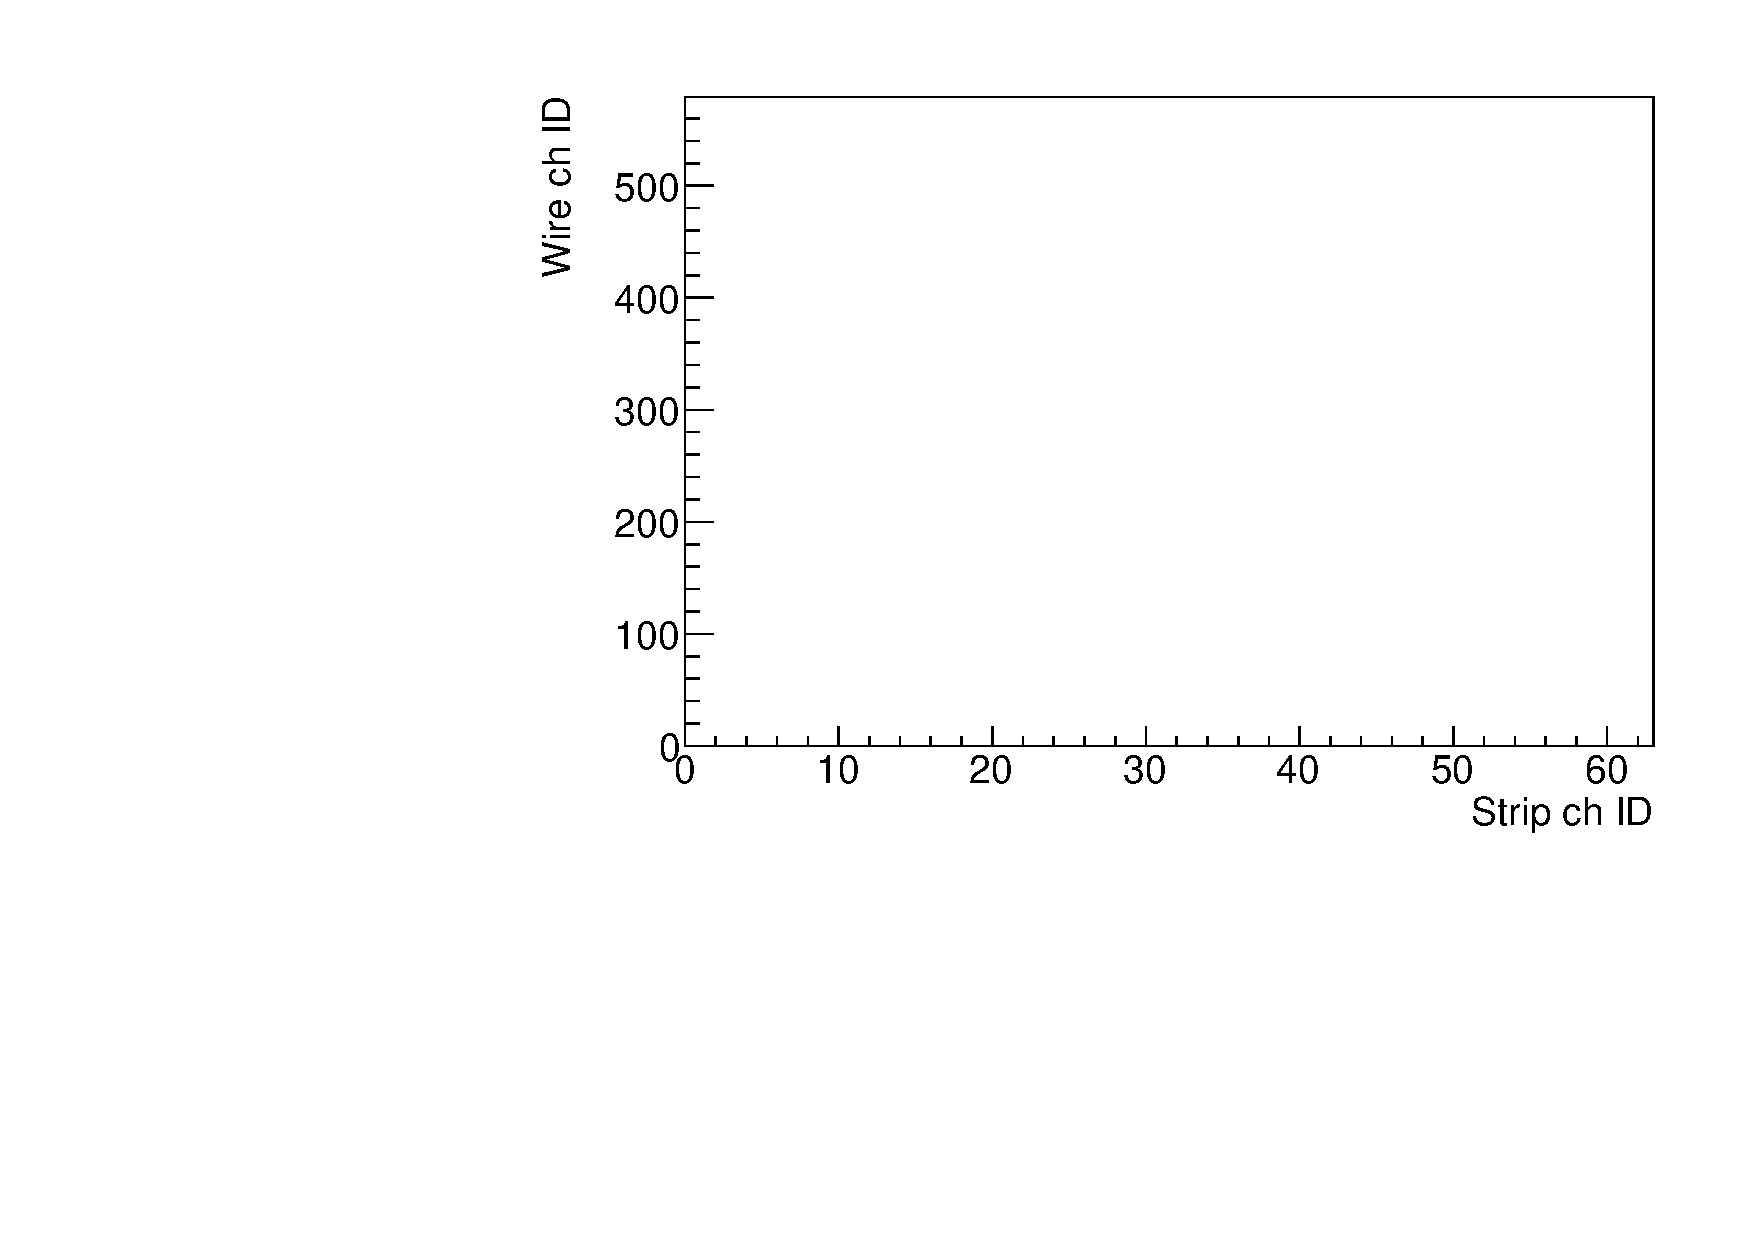
\includegraphics[height=5.6cm]{fig/Test/A_InfEC0_strip.pdf}
        \subcaption{エンドキャップ$\phi\,$0領域の結果}
    \end{minipage}
    \begin{minipage}[b]{.5\linewidth}
        \centering
        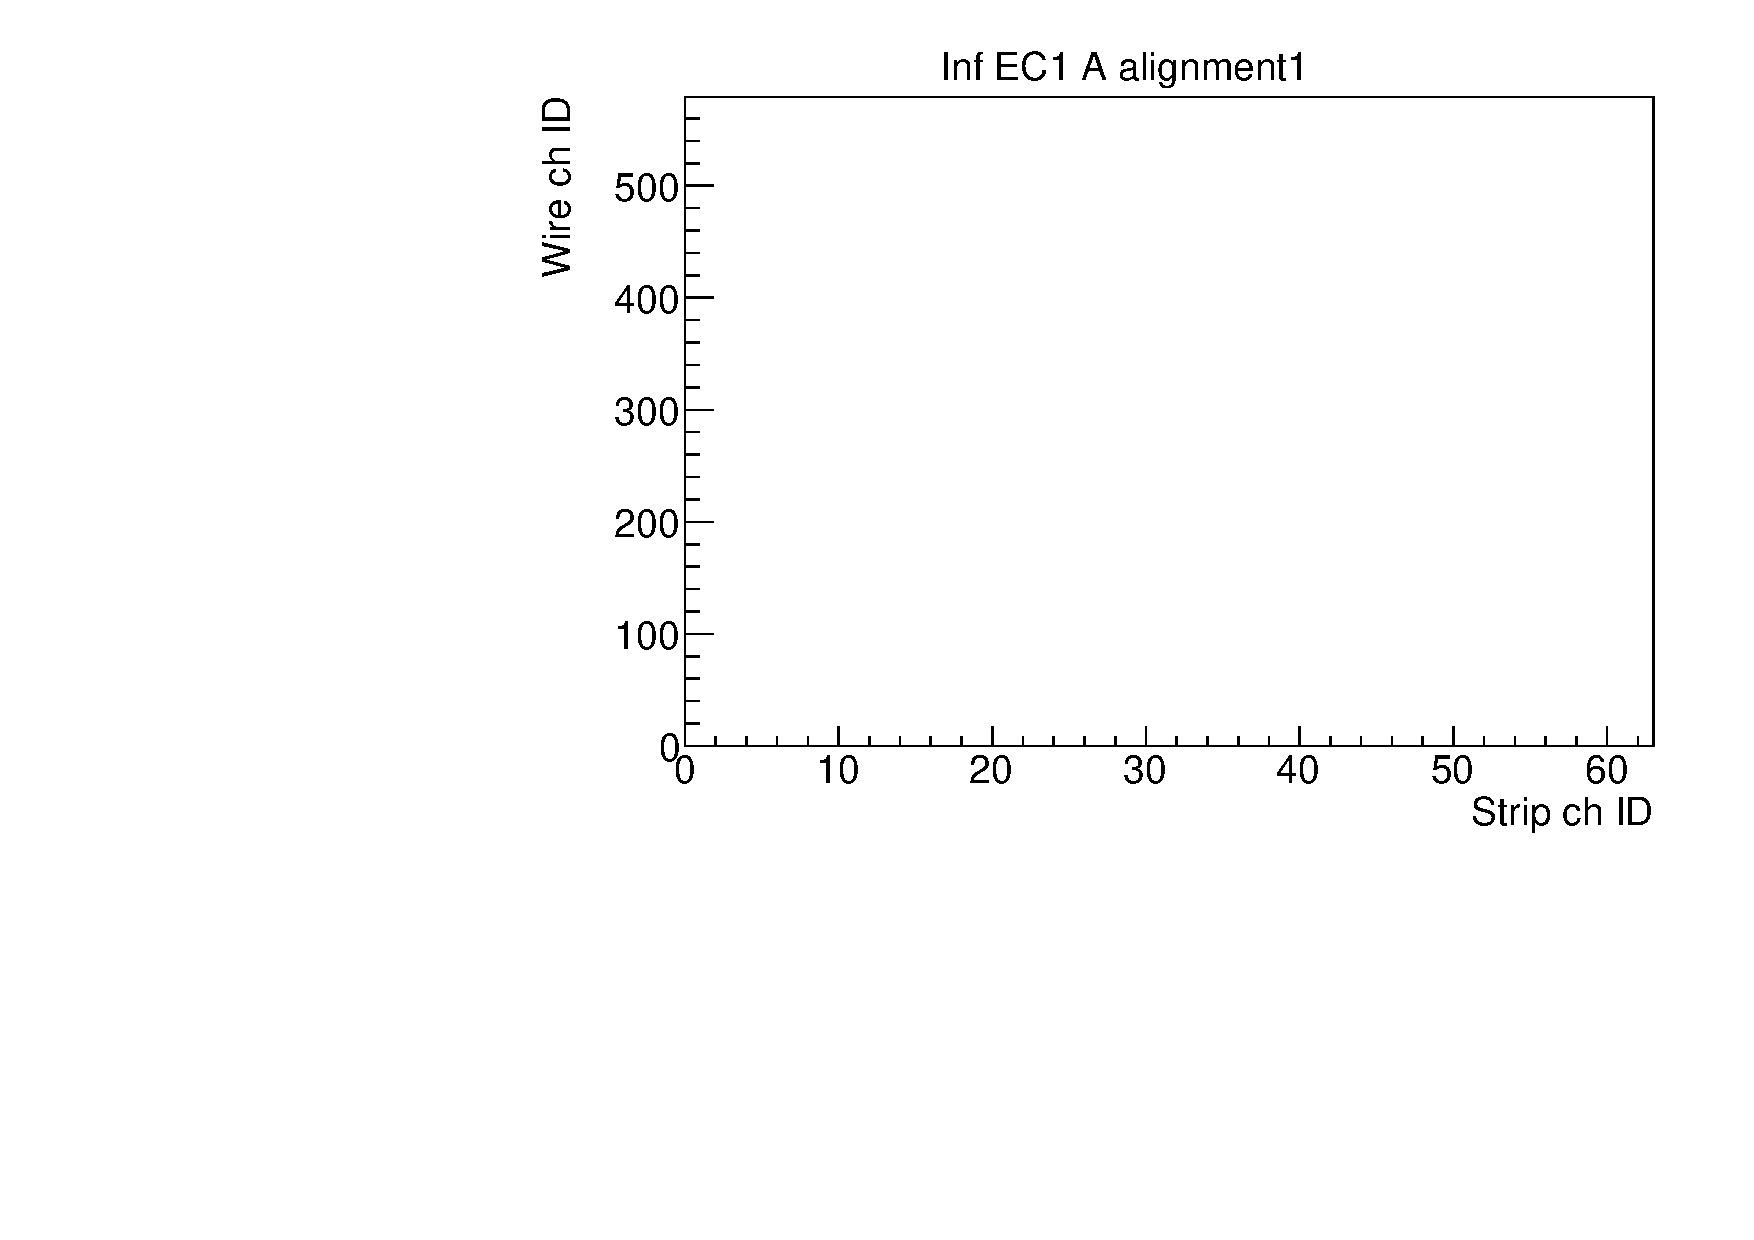
\includegraphics[height=5.6cm]{fig/Test/A_InfEC1_strip.pdf}
        \subcaption{エンドキャップ$\phi\,$1領域の結果}
    \end{minipage}\\
    \begin{minipage}[b]{\linewidth}
        \centering
        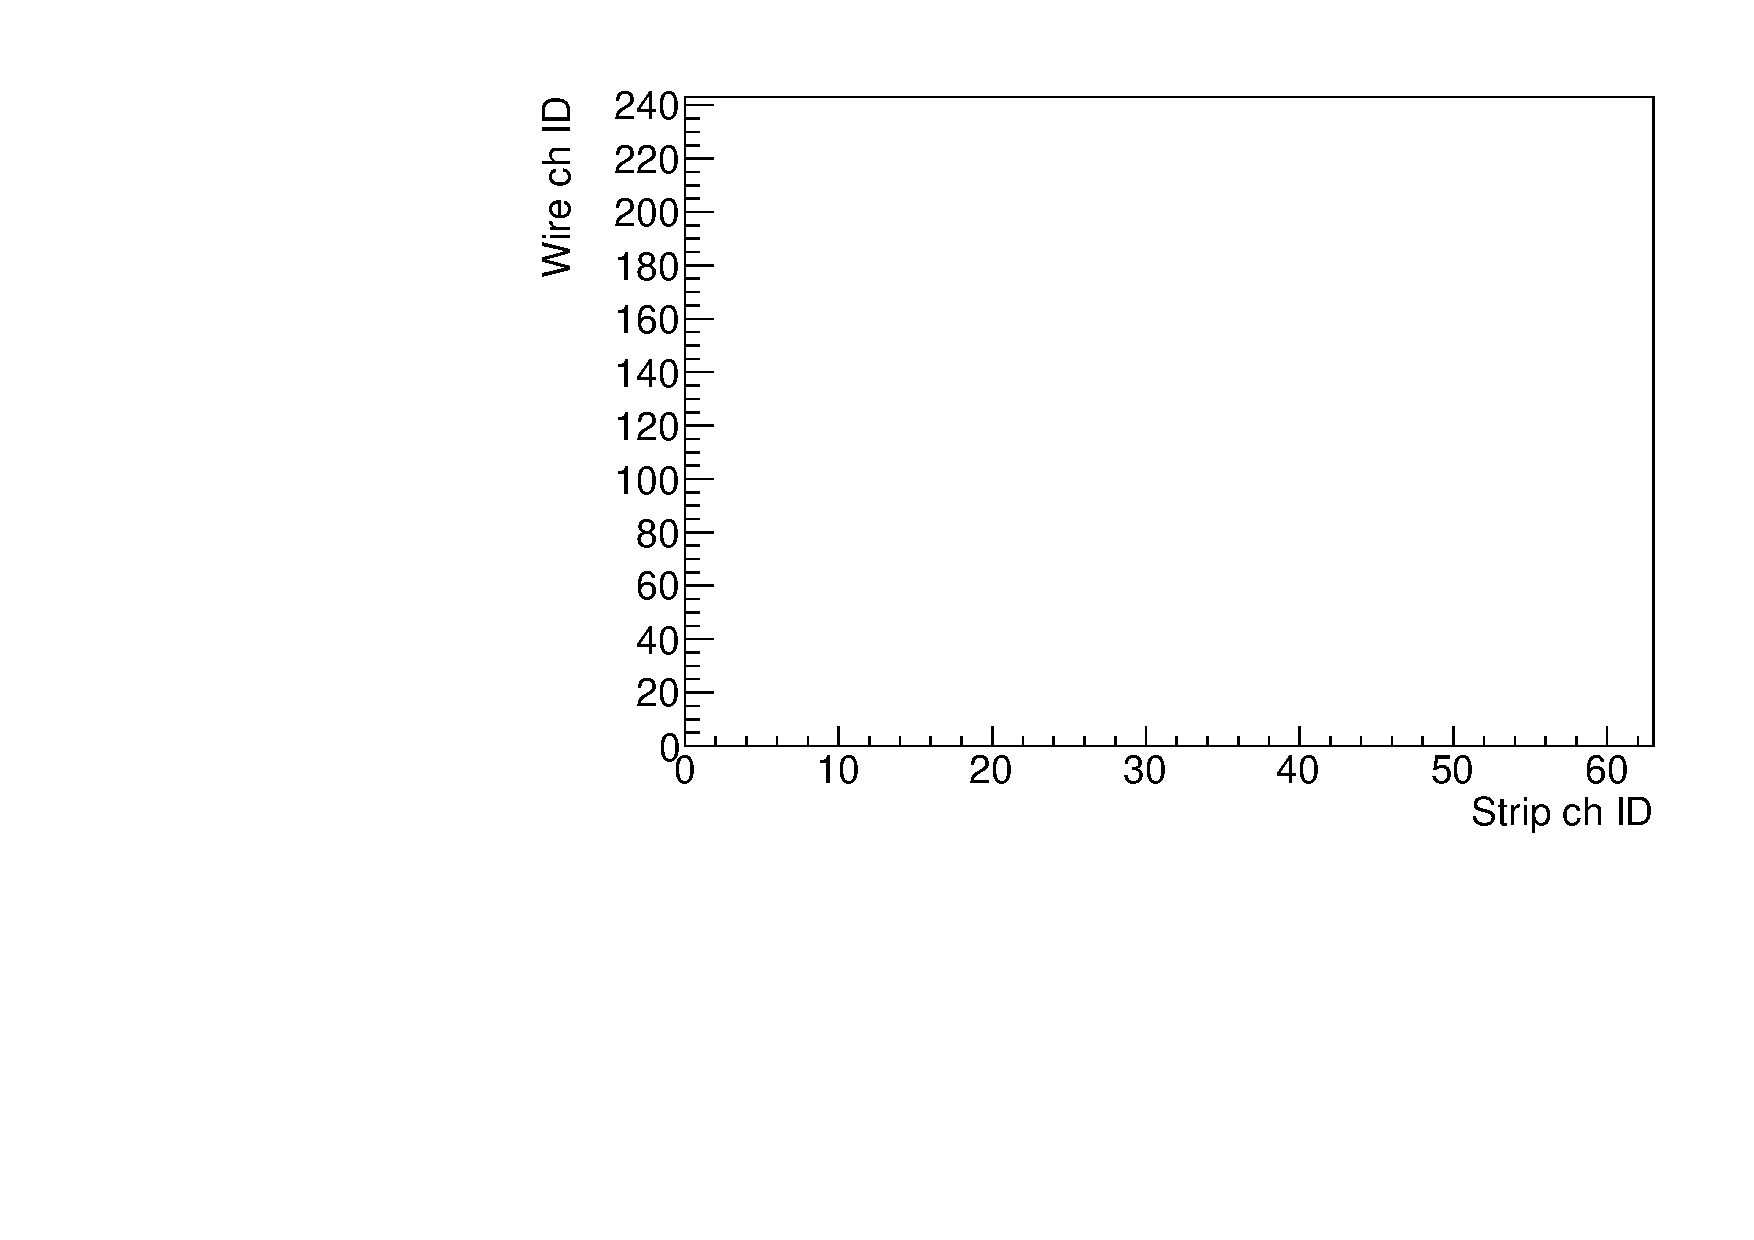
\includegraphics[height=5.6cm]{fig/Test/A_InfFW_strip.pdf}
        \subcaption{フォワード領域の結果}
    \end{minipage}
    \caption[異なる画像形式の比較]{無限運動量飛跡に対する、Strip Segment Reconstructionの応答。横軸にM3におけるStripのスタッガードID、縦軸にM3におけるWireのスタッガードIDをとる。各2次元格子点をピボットとする無限運動量飛跡を実機試験システムに投入し、$0 \leq \Delta\phi$を再構成できた場合にはその格子点を白色、できなかった場合は黒色で塗り潰す。この結果は、全ての2次元格子点で飛跡再構成に成功したことを示す。}
    \label{Inf_A_Strip}
\end{figure}

\subsubsection*{Wire Segment Reconstructionの結果}
Wire Segment Reconstructionでは、フォワード領域で99.9 \% ( 15,287 / 15,309 )、エンドキャップ$\phi\,$0領域で99.7 \%(35,370 / 36,477)、エンドキャップ$\phi\,$1領域で99.9 ( 36.181 / 36.477 )の飛跡再構成に成功した。しかし、全領域において特定の構造を持たない$\mathcal{O}(0.1\,\%)$のInefficiencyが観測された。\footnote{エンドキャップ$\phi\,$1領域のWire スタッガード ID $0 \sim 2$ の範囲でもInefficiencyが見られるが、これはM3とM1の$\eta$方向のカバレージの違いによるものであると理解されている。$\phi1$領域の$\eta\sim$2.0付近の領域では、M3がM1よりも広い$\eta$範囲をカバーしている。そのため、M3の代表点をピボットにしてスタッガードIDを割り振ると同じスタッガードIDをもつチャンネルでも$\eta$位置にずれが生じ、直線的な飛跡にならない。
}

このInefficiencyに関しては、Bitwiseシミュレーターでは確認されていないため、実機試験システム固有の問題であると考えられる。調査によると、飛跡再構成に失敗する格子点の位置は、データ取得のたびに変わることが判明している。失敗するイベントの割合は試験ごとに概ね一定で、Wire Segment Reconstruction では約0.1 \%である。現時点では、この問題がハードウェア上のトリガー回路自体の問題に起因するのか、それとも読み出し回路の問題に起因するのかの区別がついておらず、問題の解決には至っていない。今後、詳細な調査を進め、原因の解明と修正に努める。一方で、本研究で議論するInefficiencyは $\mathcal{O}(10 \%)$ 程度のものであるため、このInefficiencyは今後の議論には影響しないと考えられる。

この結果を得られるまでの過程で、本研究によって無限運動量飛跡生成機構に問題を発見し、修正を行った。デバッグの過程はAppendix\ref{sec:appendix:infinite-momentum-tracks}に詳述する。

\begin{figure}
    \begin{minipage}[b]{.5\linewidth}
        \centering
        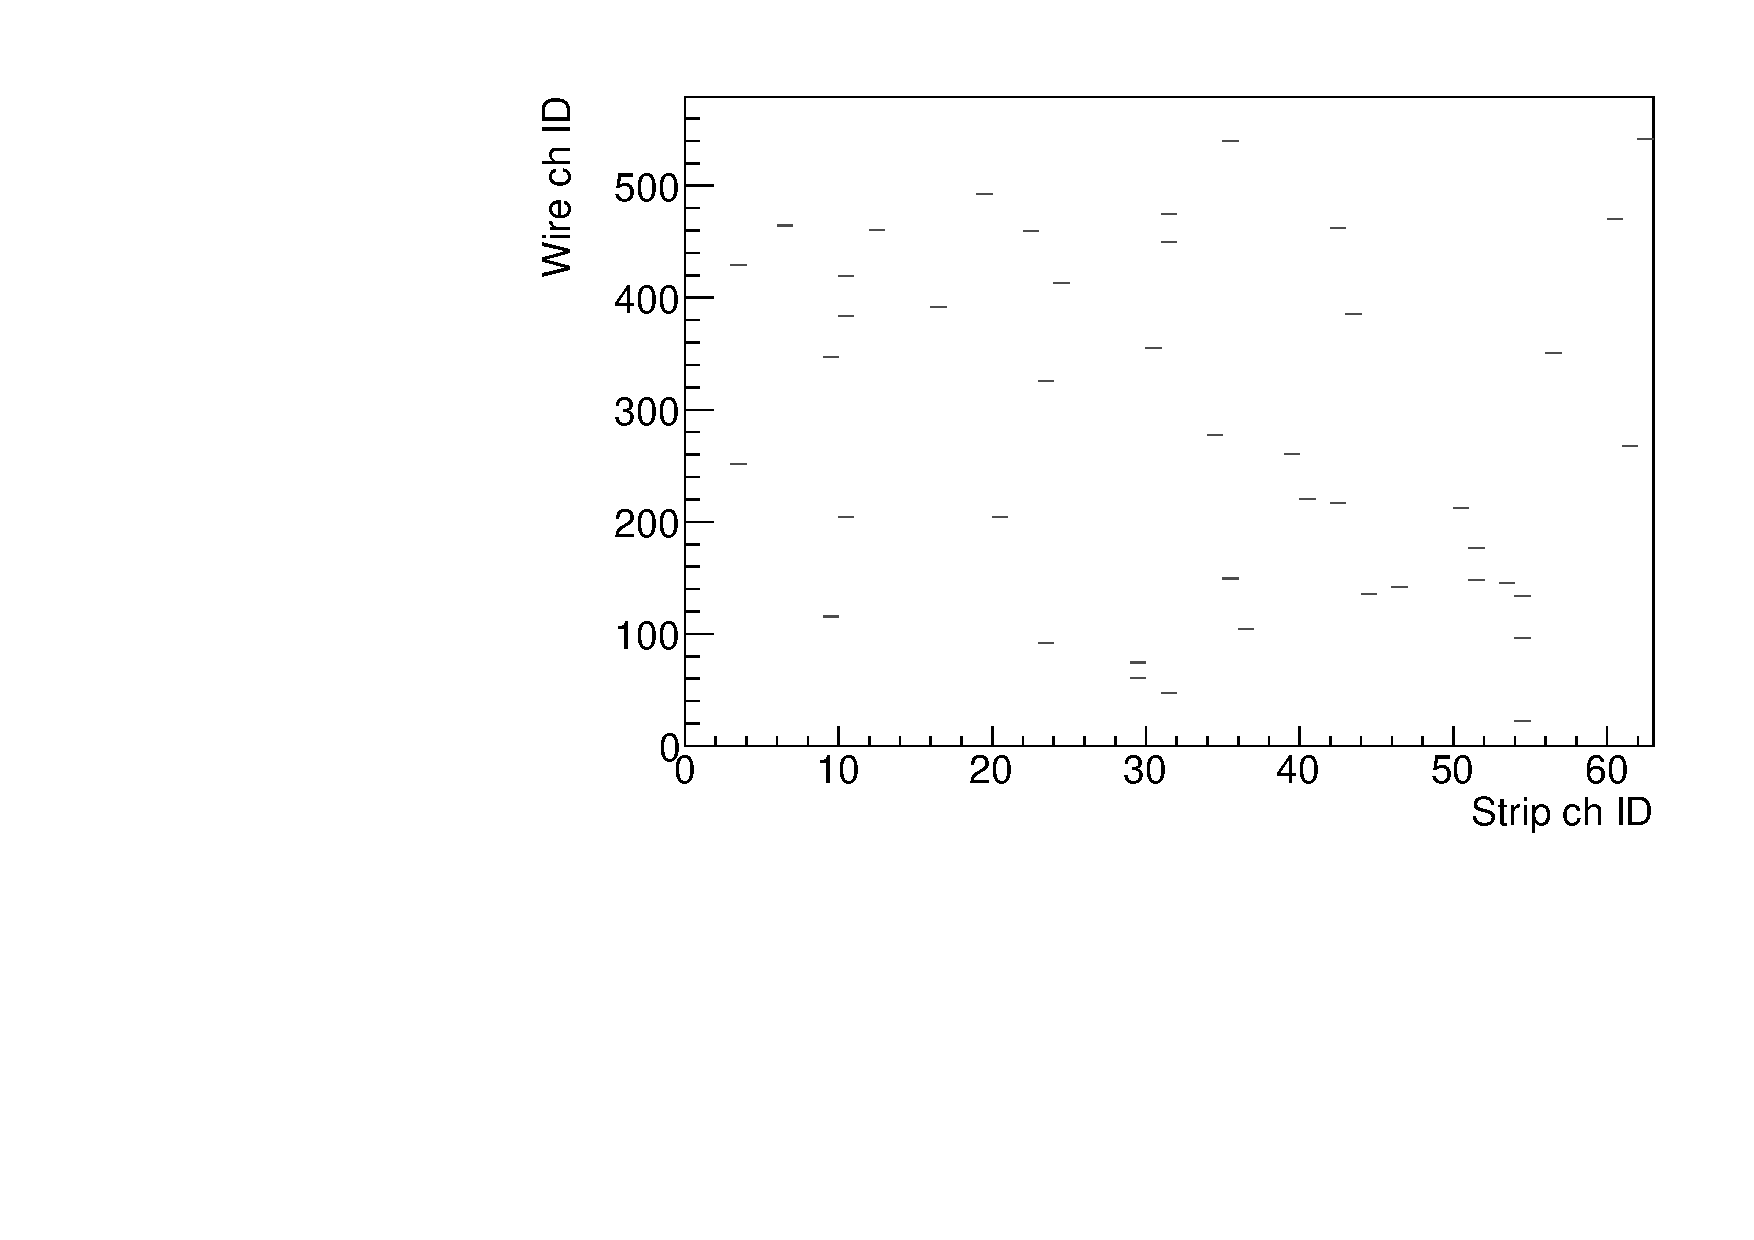
\includegraphics[height=5.6cm]{fig/Test/A_InfEC0_wire.pdf}
        \subcaption{エンドキャップ$\phi\,$0領域の結果}
    \end{minipage}
    \begin{minipage}[b]{.5\linewidth}
        \centering
        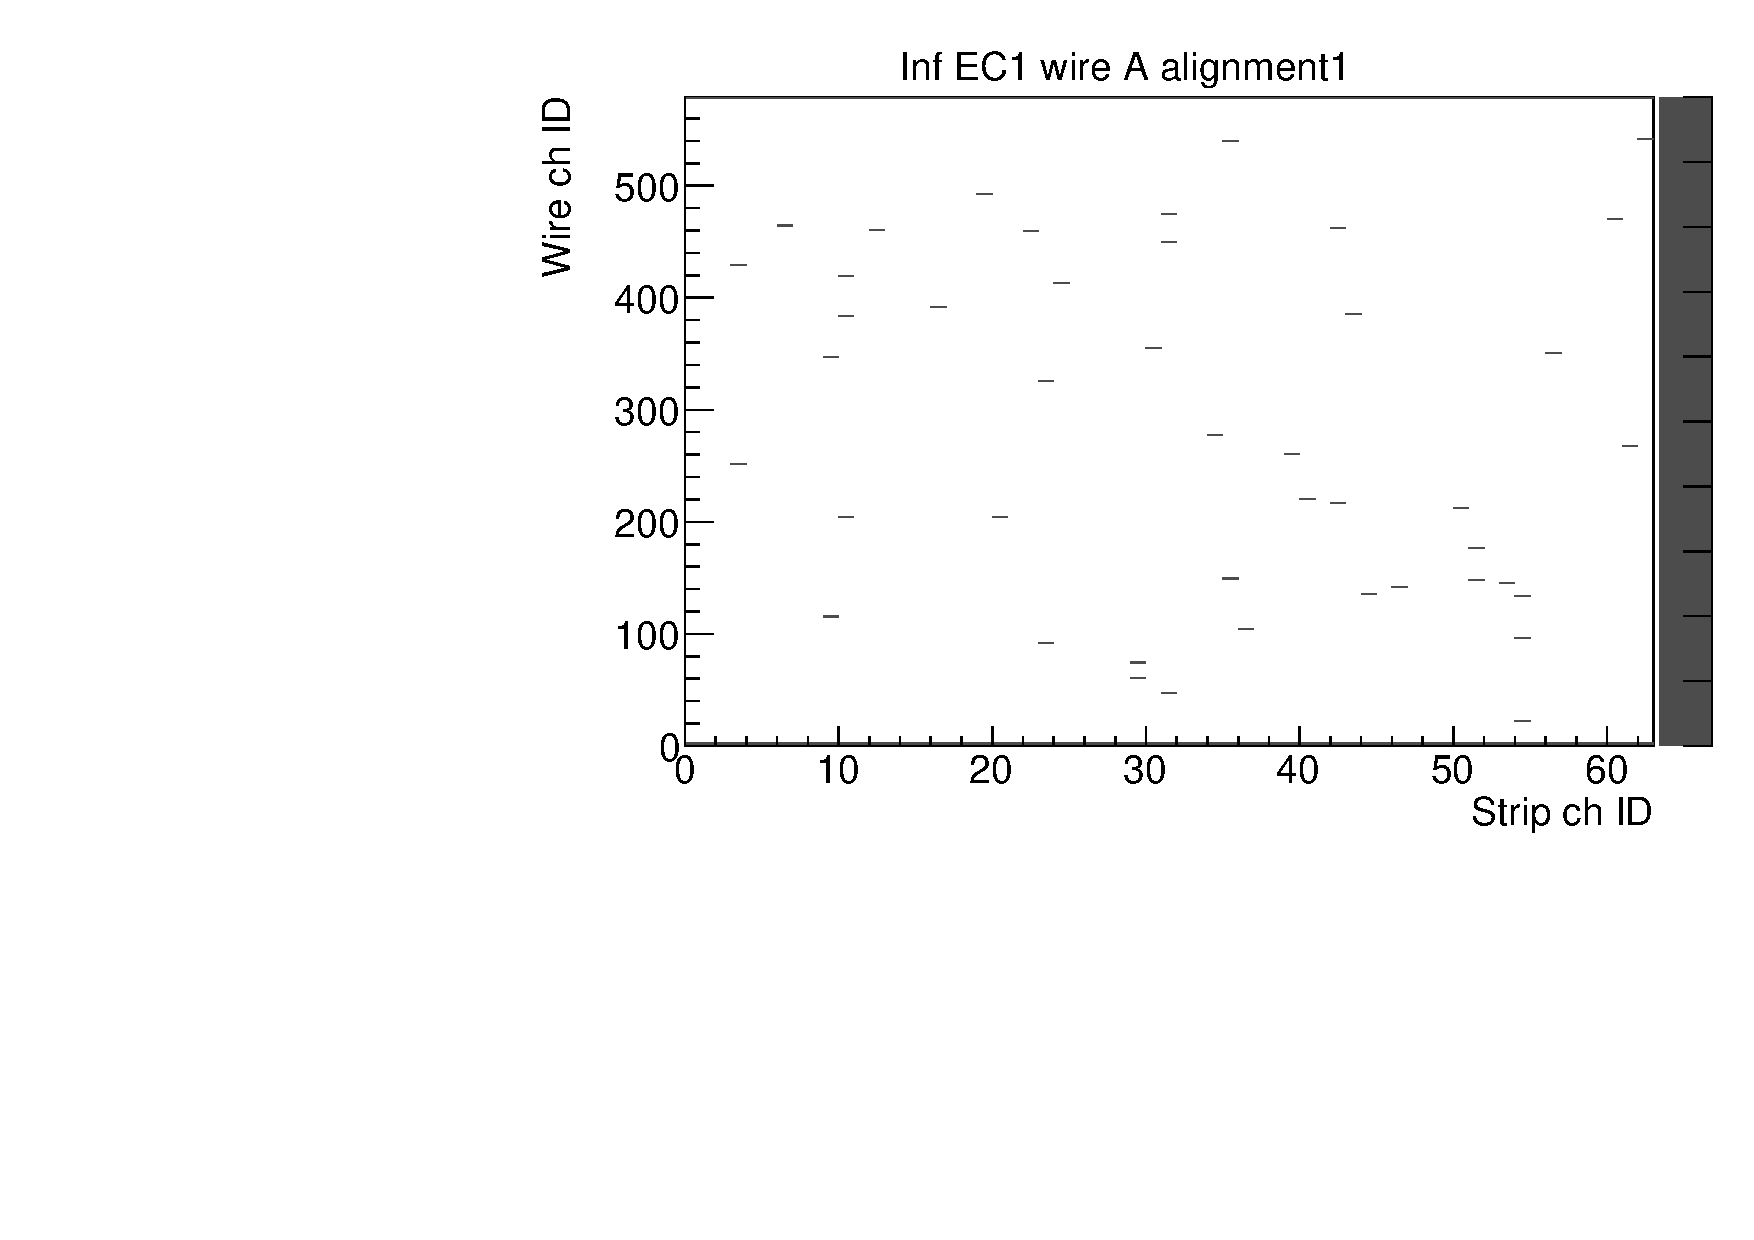
\includegraphics[height=5.6cm]{fig/Test/A_InfEC1_wire.pdf}
        \subcaption{エンドキャップ$\phi\,$1領域の結果}
    \end{minipage}\\
    \begin{minipage}[b]{\linewidth}
        \centering
        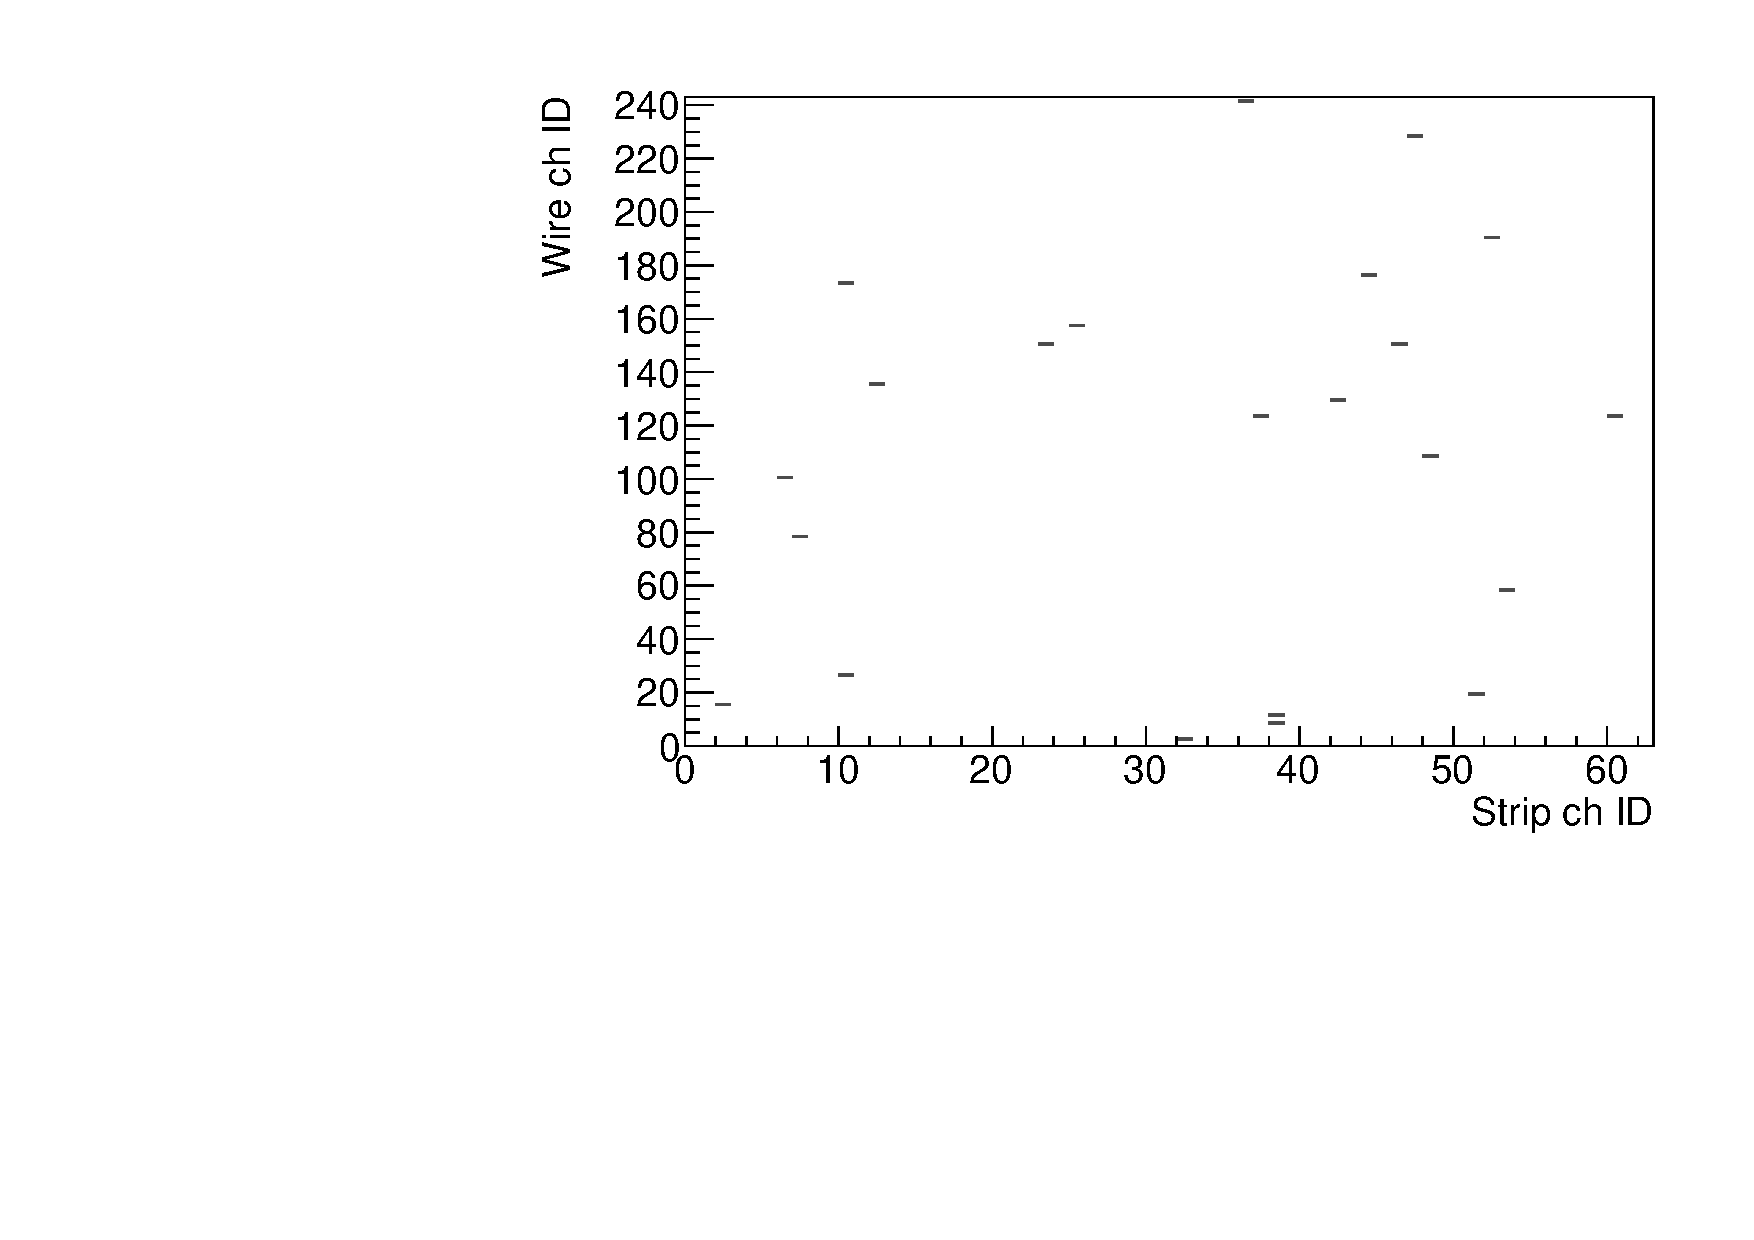
\includegraphics[height=5.6cm]{fig/Test/A_InfFW_wire.pdf}
        \subcaption{フォワード領域の結果}
    \end{minipage}
    \caption[異なる画像形式の比較]{無限運動量飛跡に対する、Wire Segment Reconstructionの応答。横軸にM3におけるStripのスタッガードID、縦軸にM3におけるWireのスタッガードIDをとる。各2次元格子点をピボットとする無限運動量飛跡を実機試験システムに投入し、$0 \leq \Delta\eta$を再構成できた場合にはその格子点を白色、できなかった場合は黒色で塗り潰す。全体の$\mathcal{O}(0.1\,\%)$程度の格子点で飛跡再構成に失敗していることがわかる。}
    \label{Inf_A_Wire}
\end{figure}


\subsubsection*{Wire Strip Coincidenceの結果}
Wire Strip Coincidence では、フォワード領域で 99.6 \% ( 15,179 / 15,309 ) 、エンドキャップ$\phi\,$0領域で 97.0 \%(35,390 / 36,477) 、エンドキャップ$\phi\,$1領域で 96.5 ( 35.201 / 36.477 ) の飛跡再構成に成功した。フォワード領域ではWire スタッガードID 190 番に該当する飛跡が全て再構成されないことが確認された。エンドキャップ領域では、Wire スタッガード ID 410 番以降の領域で、$\phi0$と$\phi1$のどちらにも規則的な構造を持ったInefficiencyが観測された。このInefficiencyは、同様のLUTを利用しているBitwiseシミュレーターでは再現されないため、LUTの原因ではなく論理回路の問題であると考えられる。Wire Strip Coincidence ではWire スタッガード IDが419より小さい領域は32 Unit regionで処理され、大きい領域は8 Unit regionで処理される。そのため、この構造的なInefficiencyは8 Unit regionのファームウェアの問題である可能性が高い。今後VivadoシミュレーターとBitwiseシミュレーターの途中出力を比較し、問題が発生じている箇所を特定し、論理回路の修正を進める。

この試験により、TGC BW Coincidence の 95 \% 以上の領域でトリガーロジックが正常に動作していることを確認することができた。一方で、Wire Strip Coincidenceでは、トリガーロジックの論理回路実装中に発生したと思われる不具合を発見することもできた。このような数 \% の局所的なInefficiencyは、網羅的かつ詳細なイベントセットを利用した本試験だからこそ見つけられたもので、従来のVivadoシミュレーターでは統計量に制約されて見つけることが困難な問題であった。任意の位置に入射するミューオン飛跡を生成できる無限運動量飛跡生成機構と、ハードウェア上で実際に動作するトリガー回路に対して、大統計量の試験を行うことができる実機システムの真価が発揮された例である。これらの誤りを実験開始前に発見し、修正することは、高輝度LHC-ATLAS実験の運転初日から、最大パフォーマンスでミューオントリガーを実現する上で非常に重要な役割を果たす。

\begin{figure}
    \begin{minipage}[b]{.5\linewidth}
        \centering
        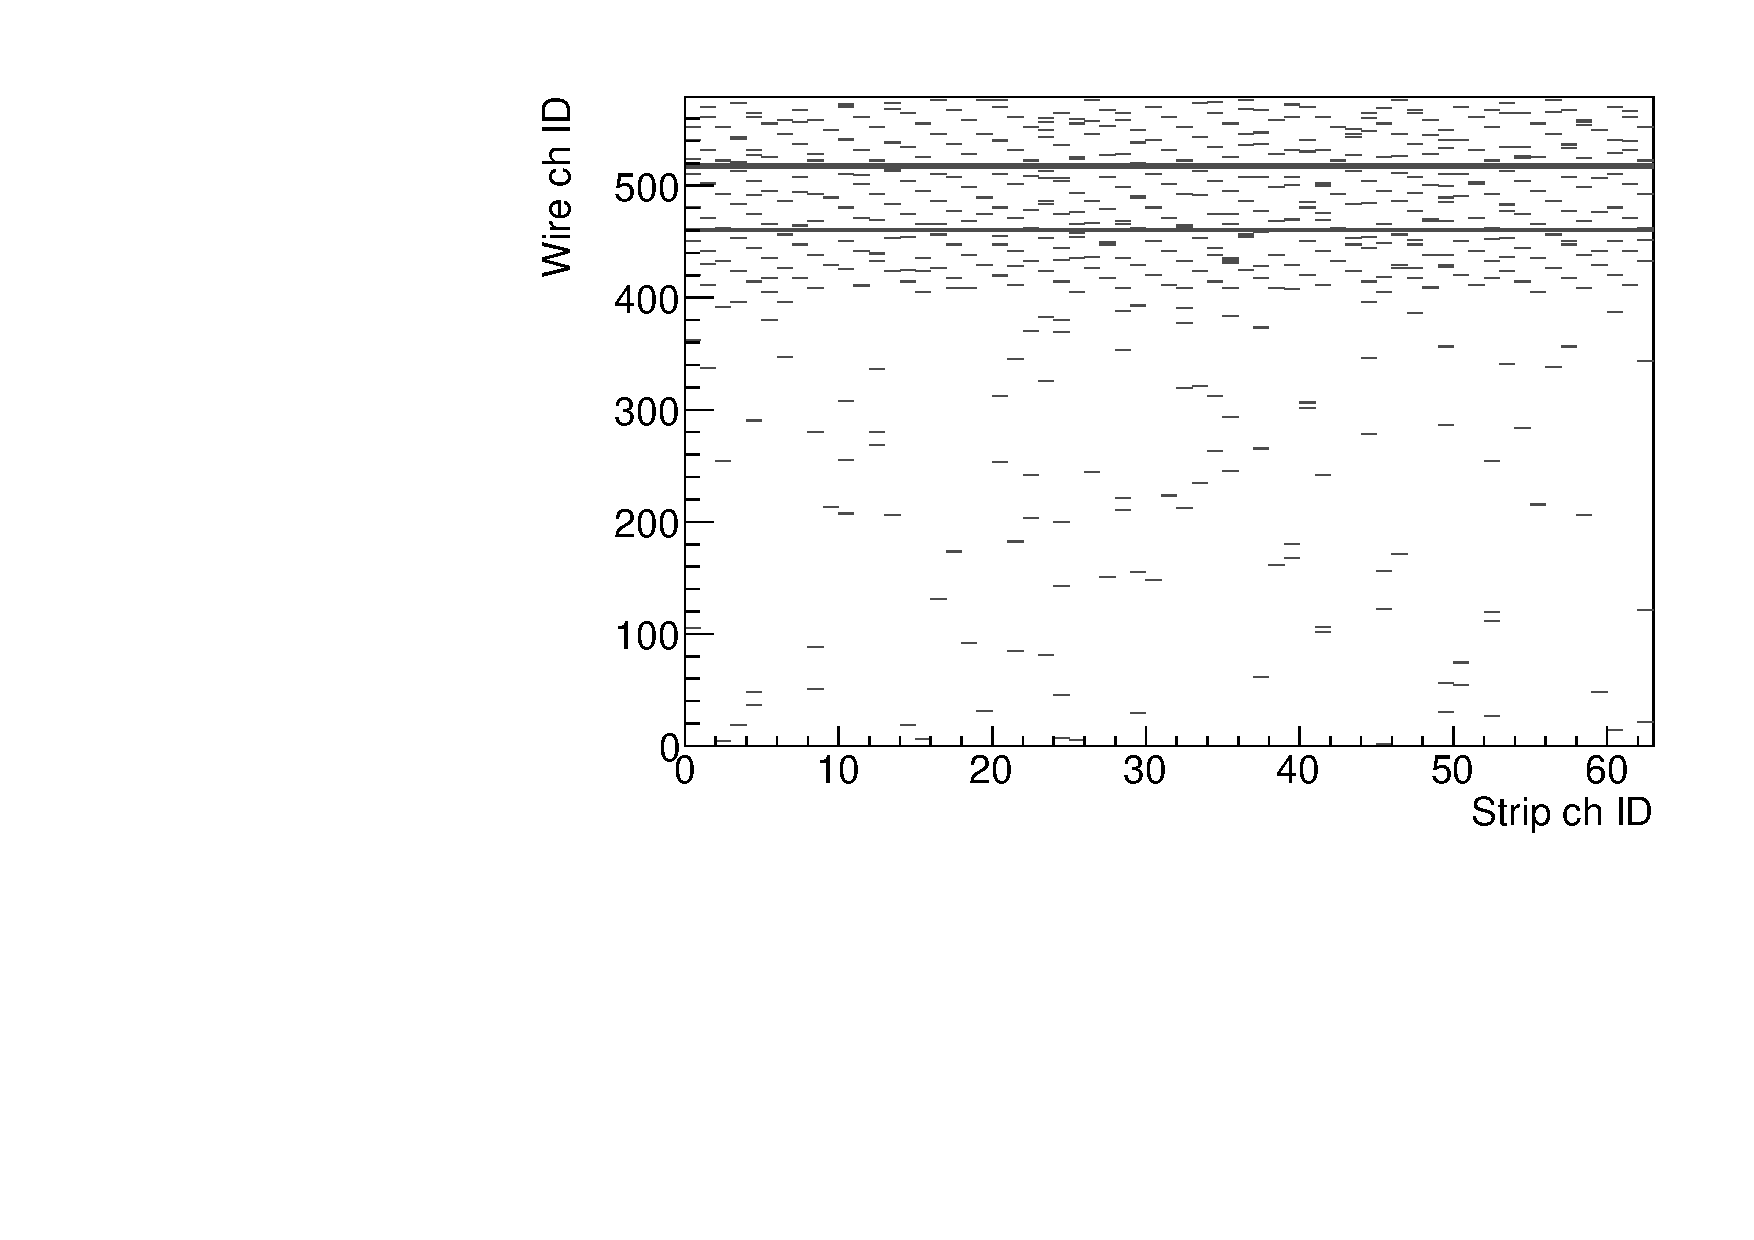
\includegraphics[height=5.6cm]{fig/Test/A_InfEC0_WS.pdf}
        \subcaption{エンドキャップ$\phi\,$0領域の結果}
    \end{minipage}
    \begin{minipage}[b]{.5\linewidth}
        \centering
        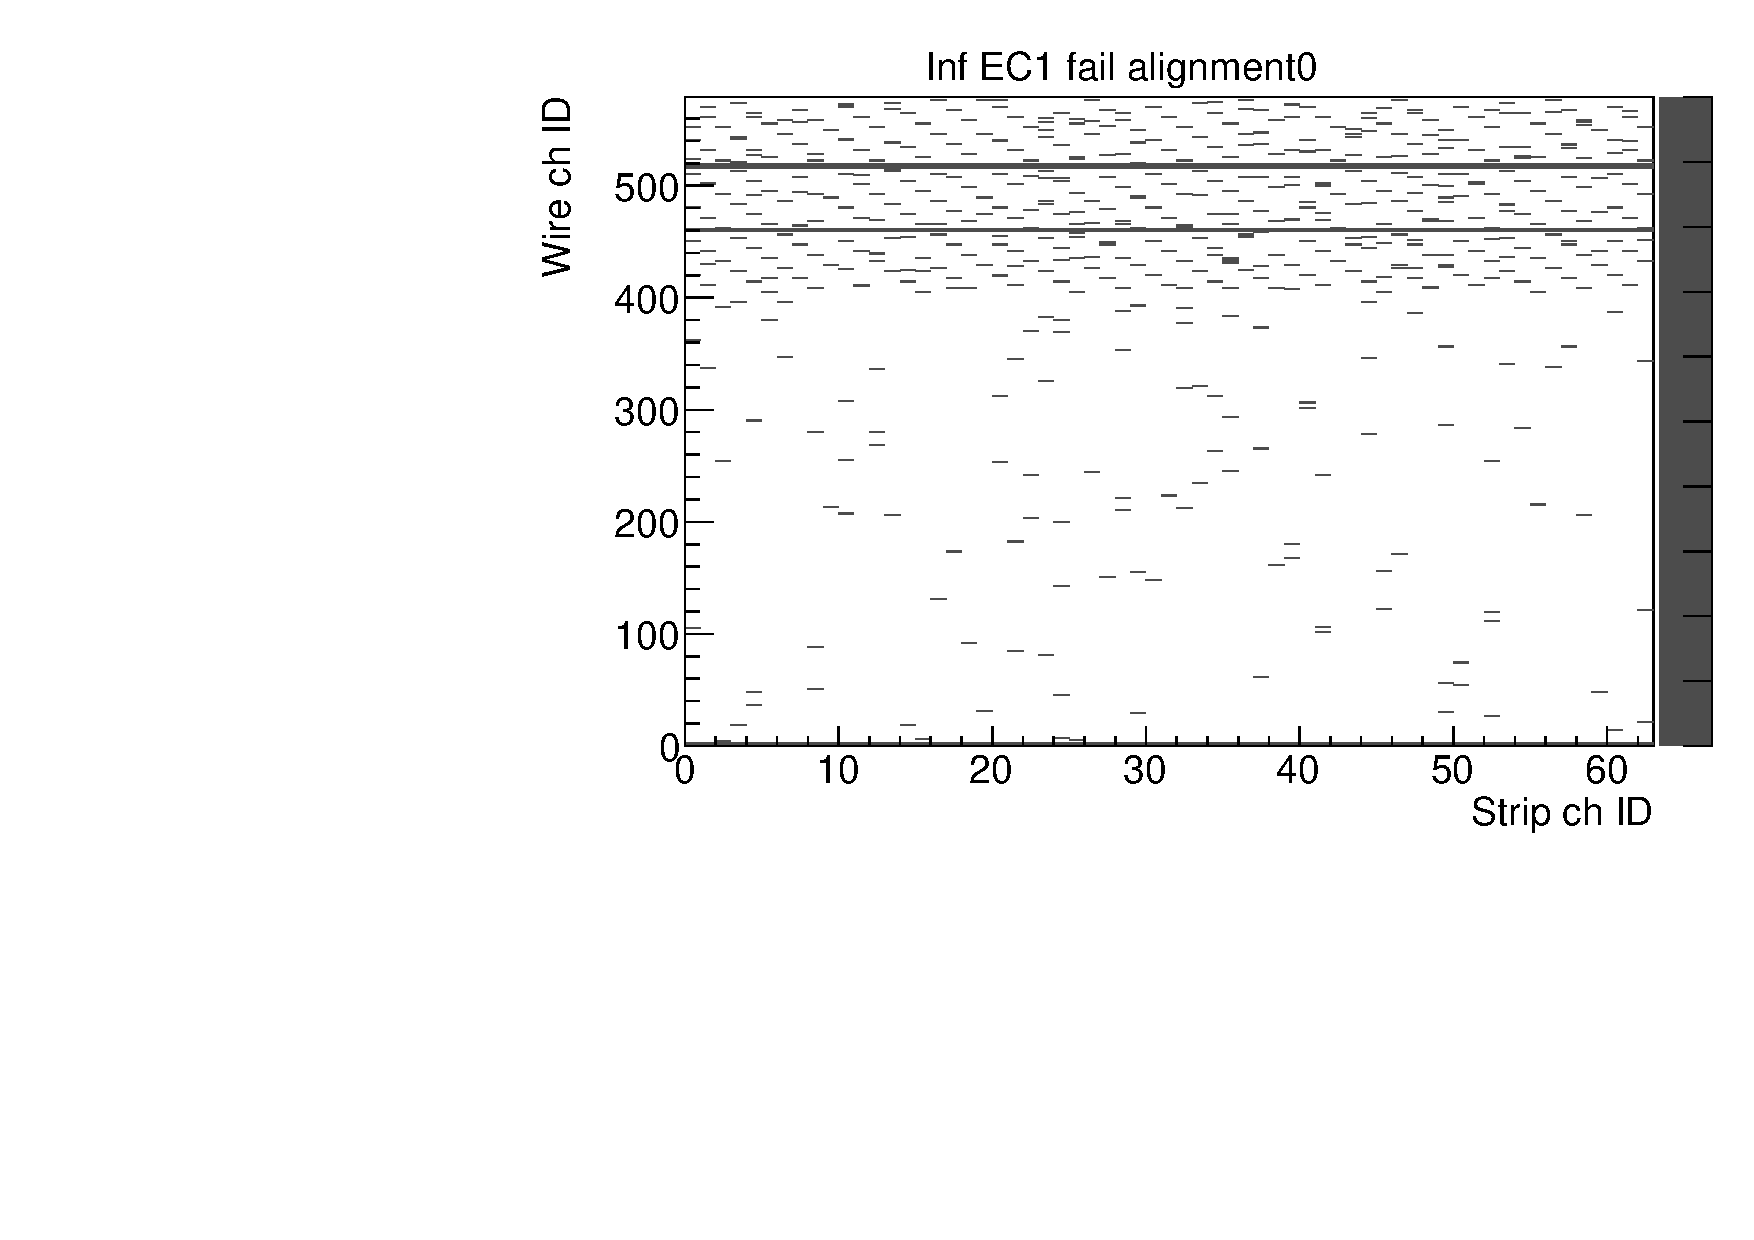
\includegraphics[height=5.6cm]{fig/Test/A_InfEC1_WS.pdf}
        \subcaption{エンドキャップ$\phi\,$1領域の結果}
    \end{minipage}\\
    \begin{minipage}[b]{\linewidth}
        \centering
        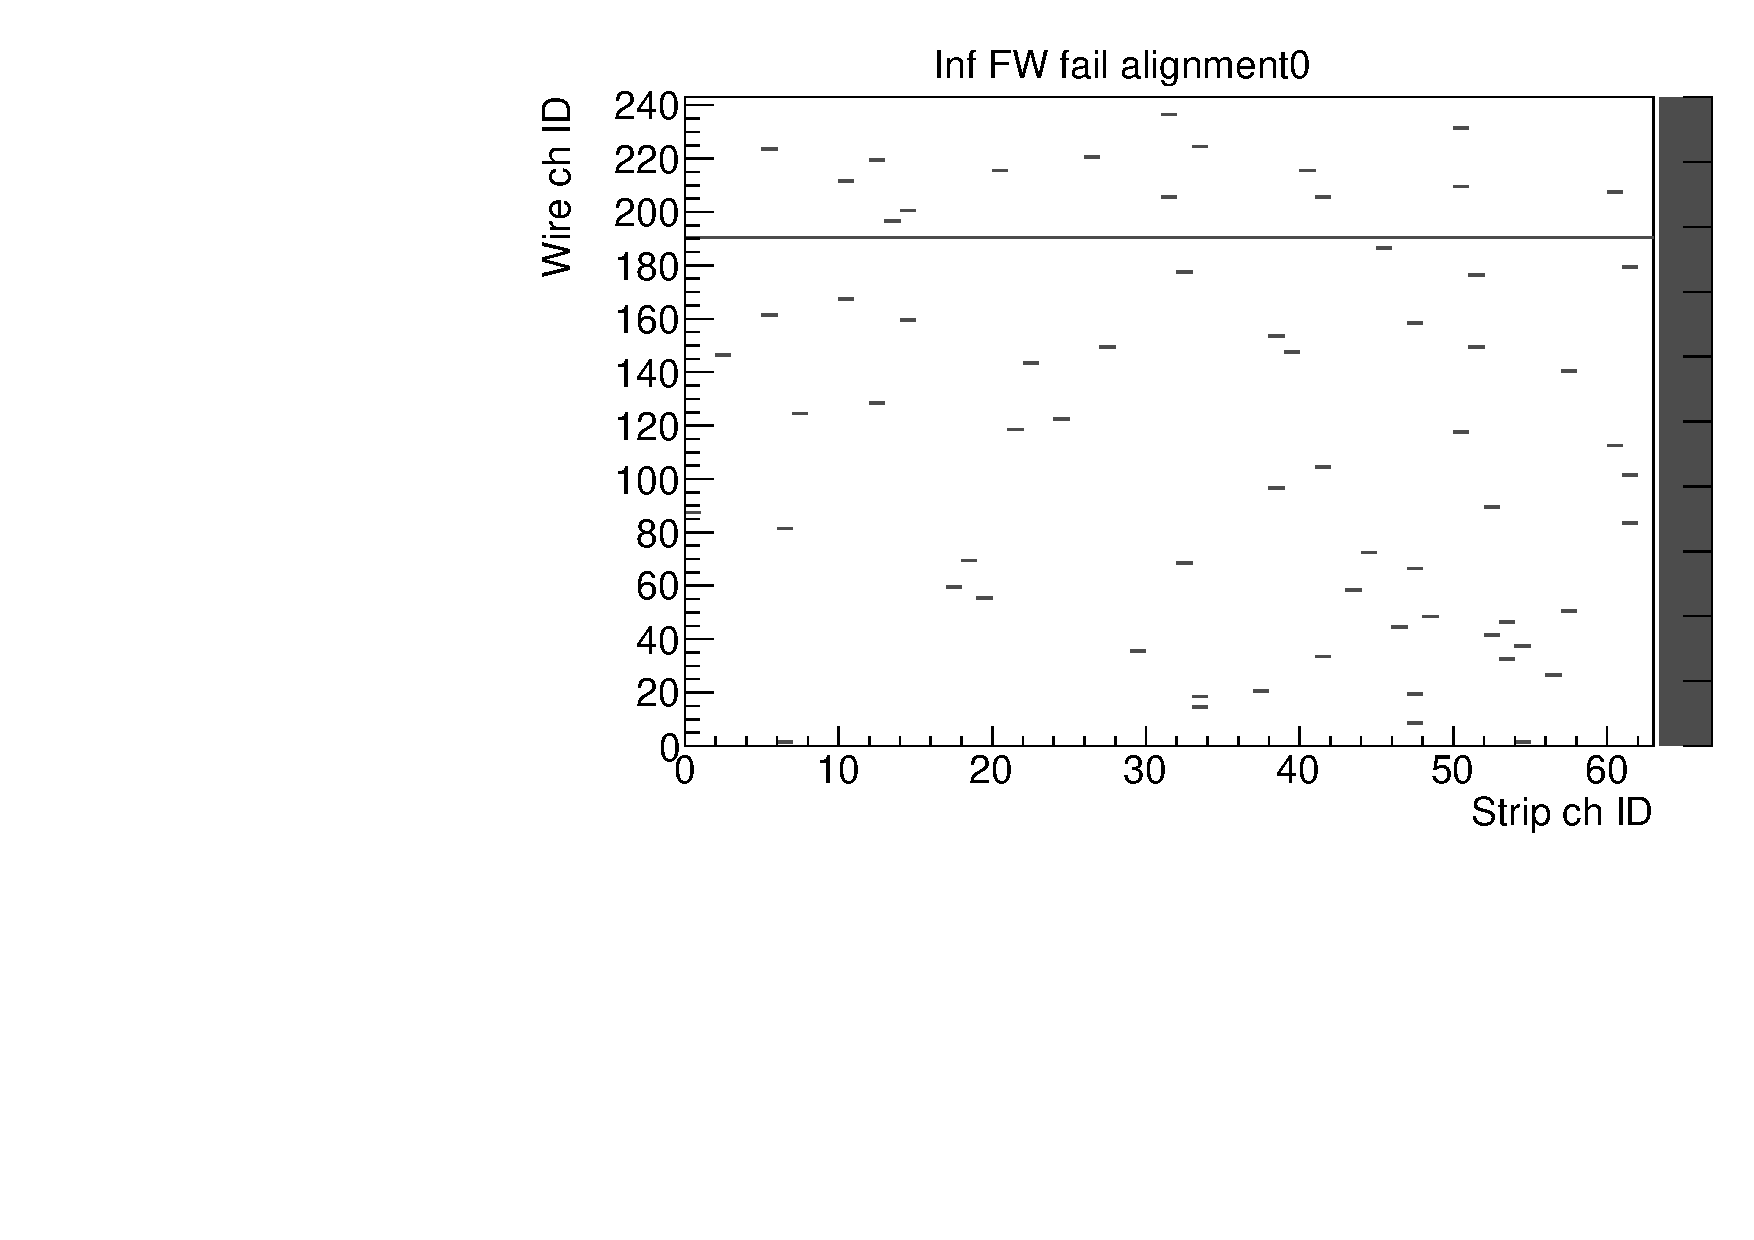
\includegraphics[height=5.6cm]{fig/Test/A_InfFW_WS.pdf}
        \subcaption{フォワード領域の結果}
    \end{minipage}
    \caption[異なる画像形式の比較]{無限運動量飛跡に対する、Wire Strip Coincidence の応答。横軸にM3におけるStripのスタッガードID、縦軸にM3におけるWireのスタッガードIDをとる。各2次元格子点をピボットとする無限運動量飛跡を実機試験システムに投入し、$0 \leq p_\mathrm{T}$を再構成できた場合にはその格子点を白色、できなかった場合は黒色で塗り潰す。Forward領域ではWire スタッガード ID 190番に該当するイベントが全て再構成に失敗している。Endcap 領域ではWire スタッガード ID 410 番以降の領域で$\phi0$と$\phi1$のどちらにも規則的な構造を持ったInefficiencyが見られる。}
    \label{Inf_A_WS}
\end{figure}

\section{モンテカルロデータを用いた性能評価}
\label{sec_SingleMuon}

本節では、より現実的なミューオンイベントに対するトリガー応答を調べるために行った、シングルミューオンモンテカルロデータを用いた試験について述べる。シングルミューオンデータとは、衝突点から検出器に1本のミューオンが入射する物理イベントをエミュレートしたデータセットである。このデータセットは、ミューオンがTGC検出器を素通りする事象、多重散乱により飛跡が曲げられる事象、制動放射や電磁シャワーによって複数のヒットが発生する事象など、実際に起こりうる物理過程を考慮したものになっている。そのため、より現実的なトリガー性能を評価することができる。用意したデータセットの概要を表\ref{tab:SingleMuon}にまとめる。本試験ではトリガー回路自体の性能に焦点を当てた検証を行うため、TGC検出器のカバー範囲外のミューオンイベントは除外している。具体的にはテストパターン作成段階で、M1、M2、M3の各ステーションに少なくても1つのヒットがあることを要求している。

本節では、シングルミューオンモンテカルロデータを用いたトリガー性能評価試験について述べる。シングルミューオンイベントとは、1本のミューオンが衝突点から検出器に入射する過程をエミュレートしたもので、ミューオンがTGC検出器を素通りする事象、多重散乱により飛跡が曲げられる事象、制動放射や電磁シャワーによってTGC検出器に複数のヒットが発生する事象など、実際に起こりうる物理過程を考慮したものになっている。そのため、無限運動量飛跡と比べてより現実的なイベントセットに対するトリガー性能を評価することができる。用意したデータセットの概要を表\ref{tab:SingleMuon}にまとめる。\pt は0 GeVから50 GeV、$\eta$、$\phi$はTGC検出器がカバーする全領域に対して満遍なく用意した。また、本試験ではトリガー回路自体の性能に焦点を当てた検証を行うため、M1、M2、M3の各ステーションに少なくても1つのヒットがあることを要求している。これにより、多重散乱で飛跡が大きく曲げられ、そもそもTGC検出器にヒットを残さないイベントなどを除外している。

\begin{table}[]
    \centering
    \caption[用意したシングルミューオンモンテカルロデータの概要]{用意したシングルミューオンモンテカルロデータの概要}
    \label{tab:SingleMuon}
    \begin{tabular}{|c|c|}
    \hline
    Parameter        &                                                                                              \\ \hline
    $p_{\mathrm{T}}$ & $ 0 \, < \, p_{\mathrm{T}}\, < 50$ GeV flat                                                  \\ \hline
    $\eta$           & 1.06 \textless |$\eta$| \textless 2.4 flat                                                   \\ \hline
    $\phi$           & 0 \textless{} $\phi$ \textless 2\pi flat                                      \\ \hline
    イベント数            & 500,000                                                                                      \\ \hline
    イベントカット          & \begin{tabular}[c]{@{}c@{}}1つのトリガーセクター内のM1、M2、M3各ステーションに\\ それぞれ1つ以上のヒットがあることを要求\end{tabular} \\ \hline
    \end{tabular}
\end{table}

\subsubsection*{Strip Segment Reconstructionのトリガー効率}
この試験では \pt  が十分に大きい事象に対するトリガー応答を確認することを目的とし、Truth \pt $\,$20 GeV 以上のミューオンに対する検出効率を評価する。Efficiencyは式\ref{eq:Strip_Efficiency}のように定義する。

\begin{equation}
    \mathrm {Efficiency} = \frac{\mathrm{Strip\,Segment \,Reconstruction\,で\Delta\phi\,を再構成できたイベント数}}{\mathrm{Truth\,pt \,20 \,GeV以上のイベント数}}
    \label{eq:Strip_Efficiency}
\end{equation}

Strip Segment Reconstructionの検出効率の$\eta$および$\phi$依存性を図\ref{SM_A_strip}に示す。黒色の点はSL実機システムの出力結果、赤色の点はBitwise シミュレーターの出力結果を表している。全領域での平均トリガー検出効率は 97.4 \%であり、先行研究のソフトウェアシミュレーションの結果と矛盾のない結果が得られた。

トリガー効率の$\phi$依存性を見ると、チェンバーとチェンバーの境界に位置する領域 (エンドキャップ領域ではTGC BW 1周を48のトリガーセクターで分割するので 2$\pi$ / 48 = 0.26 おきにチェンバーの境界が存在する) でEfficiencyが15 \%程度下がる傾向が確認された。このイベントセットでは事前に3つのステーションにヒットがあることを要求しているため、原理的にはチェンバー境界であってもEfficiencyが下がることはない。このInefficiencyはBitwiseシミュレーターでも再現されていることから、ファームウェアに固有の問題ではなく、共通に使用しているLUTの不具合に起因するものであると考えられる。
今後、Bitwiseシミュレーターを用いて、イベントごとに飛跡再構成が失敗した理由を調査し、修正する。

また、Strip Segment Reconstructionでは実機とBitwiseシミュレーターの結果が概ね一致している。これはBitwiseシミュレーターが論理回路のロジックを極めて正確に再現できていることを示している。しかし、2 < $\eta$のフォワード領域の、特に$\phi$チェンバー境界領域で、両者の出力に違いが生じている。原理的にはこの2つの出力は完全に一致するべきものであり、この差異はBitwiseシミュレーターとファームウェアでチェンバー境界の取扱い方に、わずかな違いがあることを示唆している。今後、両者のロジックを精密に比較し、出力の不一致を解消していく。

\begin{figure}
\begin{minipage}[b]{\linewidth}
\centering
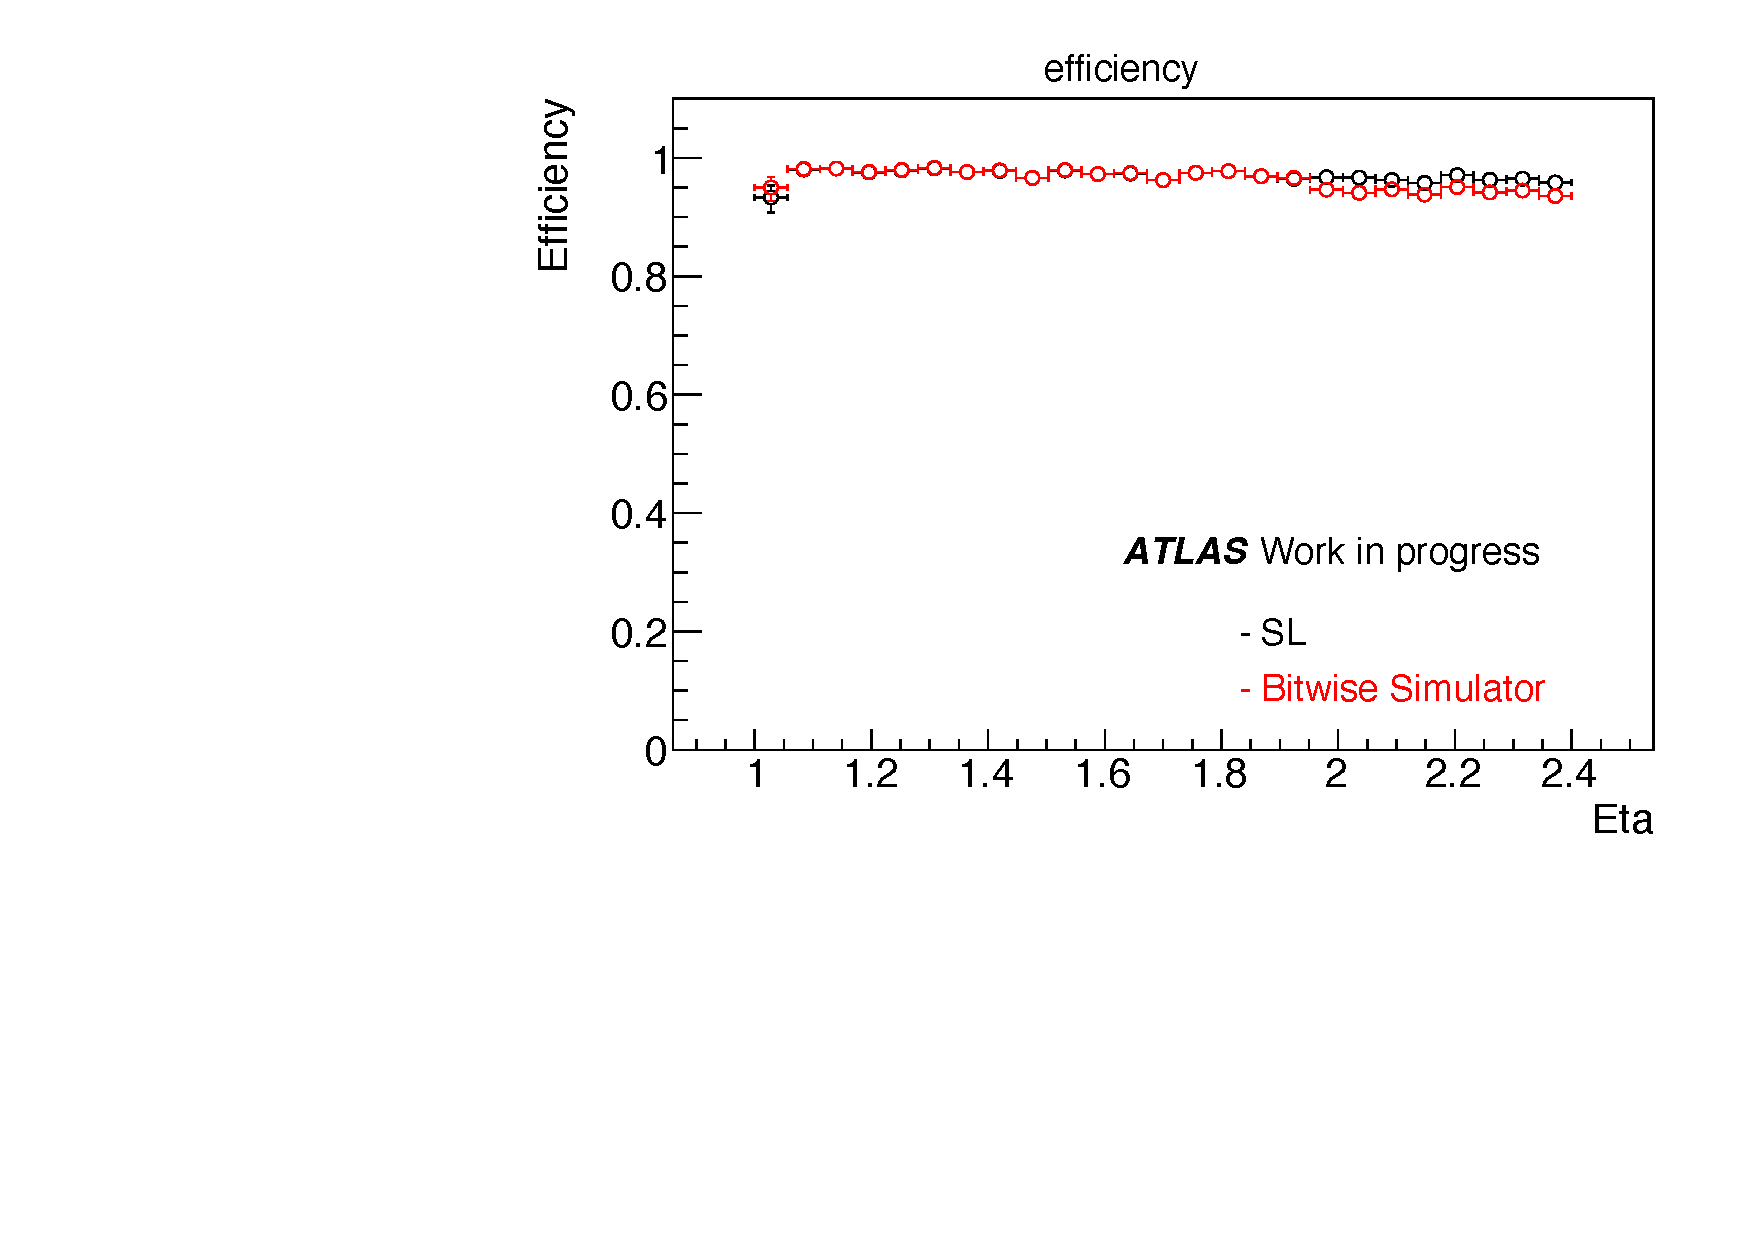
\includegraphics[height=10cm]{fig/Test/A_SM_strip_eta.pdf}
\subcaption{Strip Segment Reconstructino 検出効率の$\eta$依存性}
\end{minipage}\\
\begin{minipage}[b]{\linewidth}
\centering
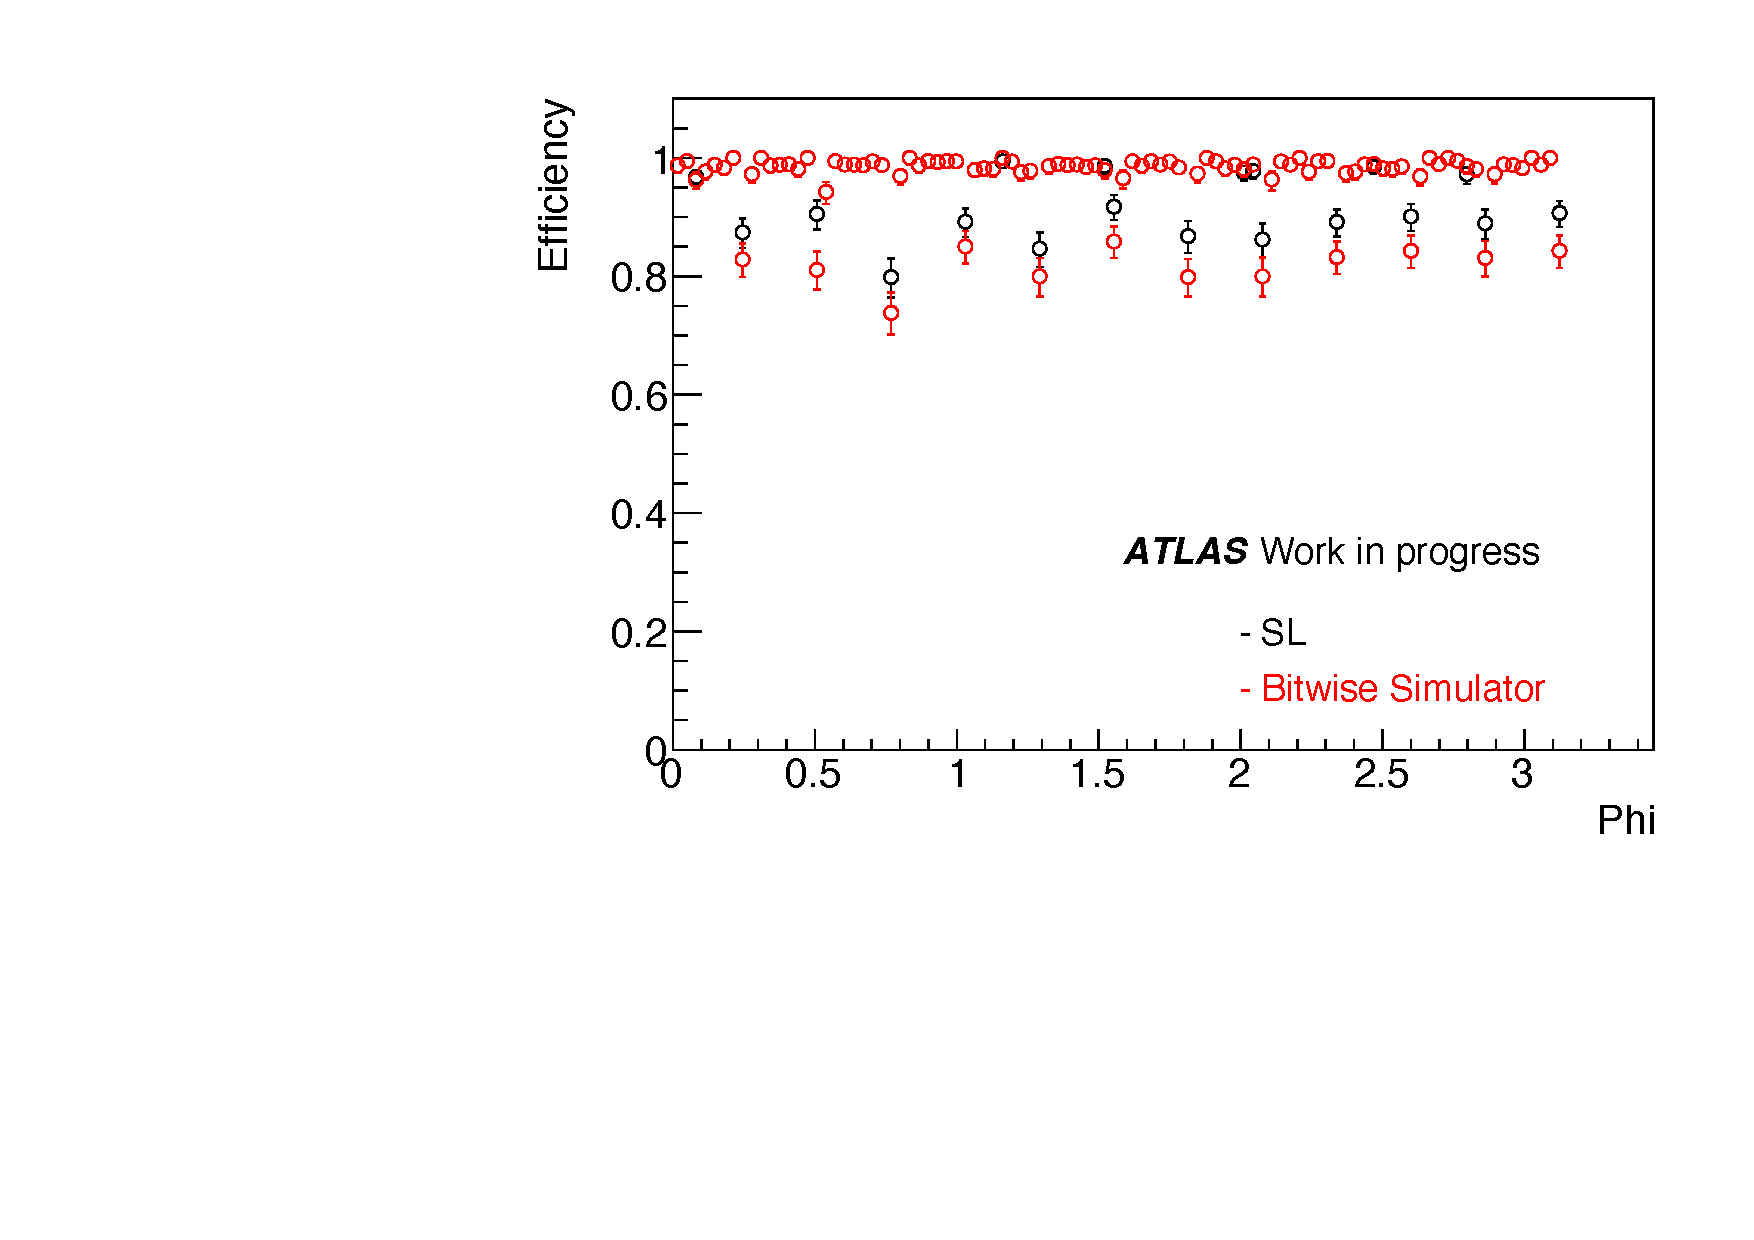
\includegraphics[height=10cm]{fig/Test/A_SM_strip_phi.pdf}
\subcaption{Strip Segment Reconstructino 検出効率の$\phi$依存性}
\end{minipage}%
\caption[Strip Segment Reconstructionの検出効率]{Strip Segment Reconstructionの検出効率。黒色のプロットが実機出力、赤色のプロットがBitwiseシミュレータの出力を表す。全領域のトリガー検出効率は97.4 \%であり、先行研究のソフトウェアシミュレーションと矛盾のない結果が得られた。トリガー効率の$\phi$依存性に着目すると、実機試験システムでもBitiwiseシミュレーターでも、チェンバー境界領域で10 \%程度のInefficiencyが見られる。また、フォワード領域の、特にチェンバー境界領域で実機とBitwiseシミュレーターで出力が一致していないイベントが数 \%程度存在している。}
\label{SM_A_strip}
\end{figure}



\subsubsection{Wire Segment Reconstructionのトリガー効率}
\par
Stripの場合と同様に、Efficiencyは式\ref{eq:Wire_Efficiency}のように定義する。

\begin{equation}
    \mathrm {Efficiency} = \frac{\mathrm{Wire\,Segment \,Reconstruction\,で\Delta\eta\,を再構成できたイベント数}}{\mathrm{Truth\,pt \,20 \,GeV以上のイベント数}}
    \label{eq:Wire_Efficiency}
\end{equation}


Wire Segment Reconstructionの検出効率の$\eta$および$\phi$依存性を図\ref{SM_A_strip}に示す。全領域での平均トリガー効率は 96.3 \%であり、先行研究のソフトウェアシミュレーターやVivadoシミュレーターの結果と矛盾しない結果が得られた。

トリガー効率の$\eta$依存性に着目すると、$\eta \sim 1.4$ 付近で約5 \%のInefficiencyが見られる。このInefficiencyに対してBitwiseシミュレーターを用いた調査したところ、Wire Station Coincidence、およびWire Segment ReconstructionのAddress Specifierまでは期待通り動作していることが確認された。一方、Segment ExtractorでLUTにアクセスした結果、中身がNULLであるイベントが存在することがわかっている。今後はLUTの修正を行い、この領域のInefficiencyを改善する。

\begin{figure}
    \begin{minipage}[b]{\linewidth}
    \centering
    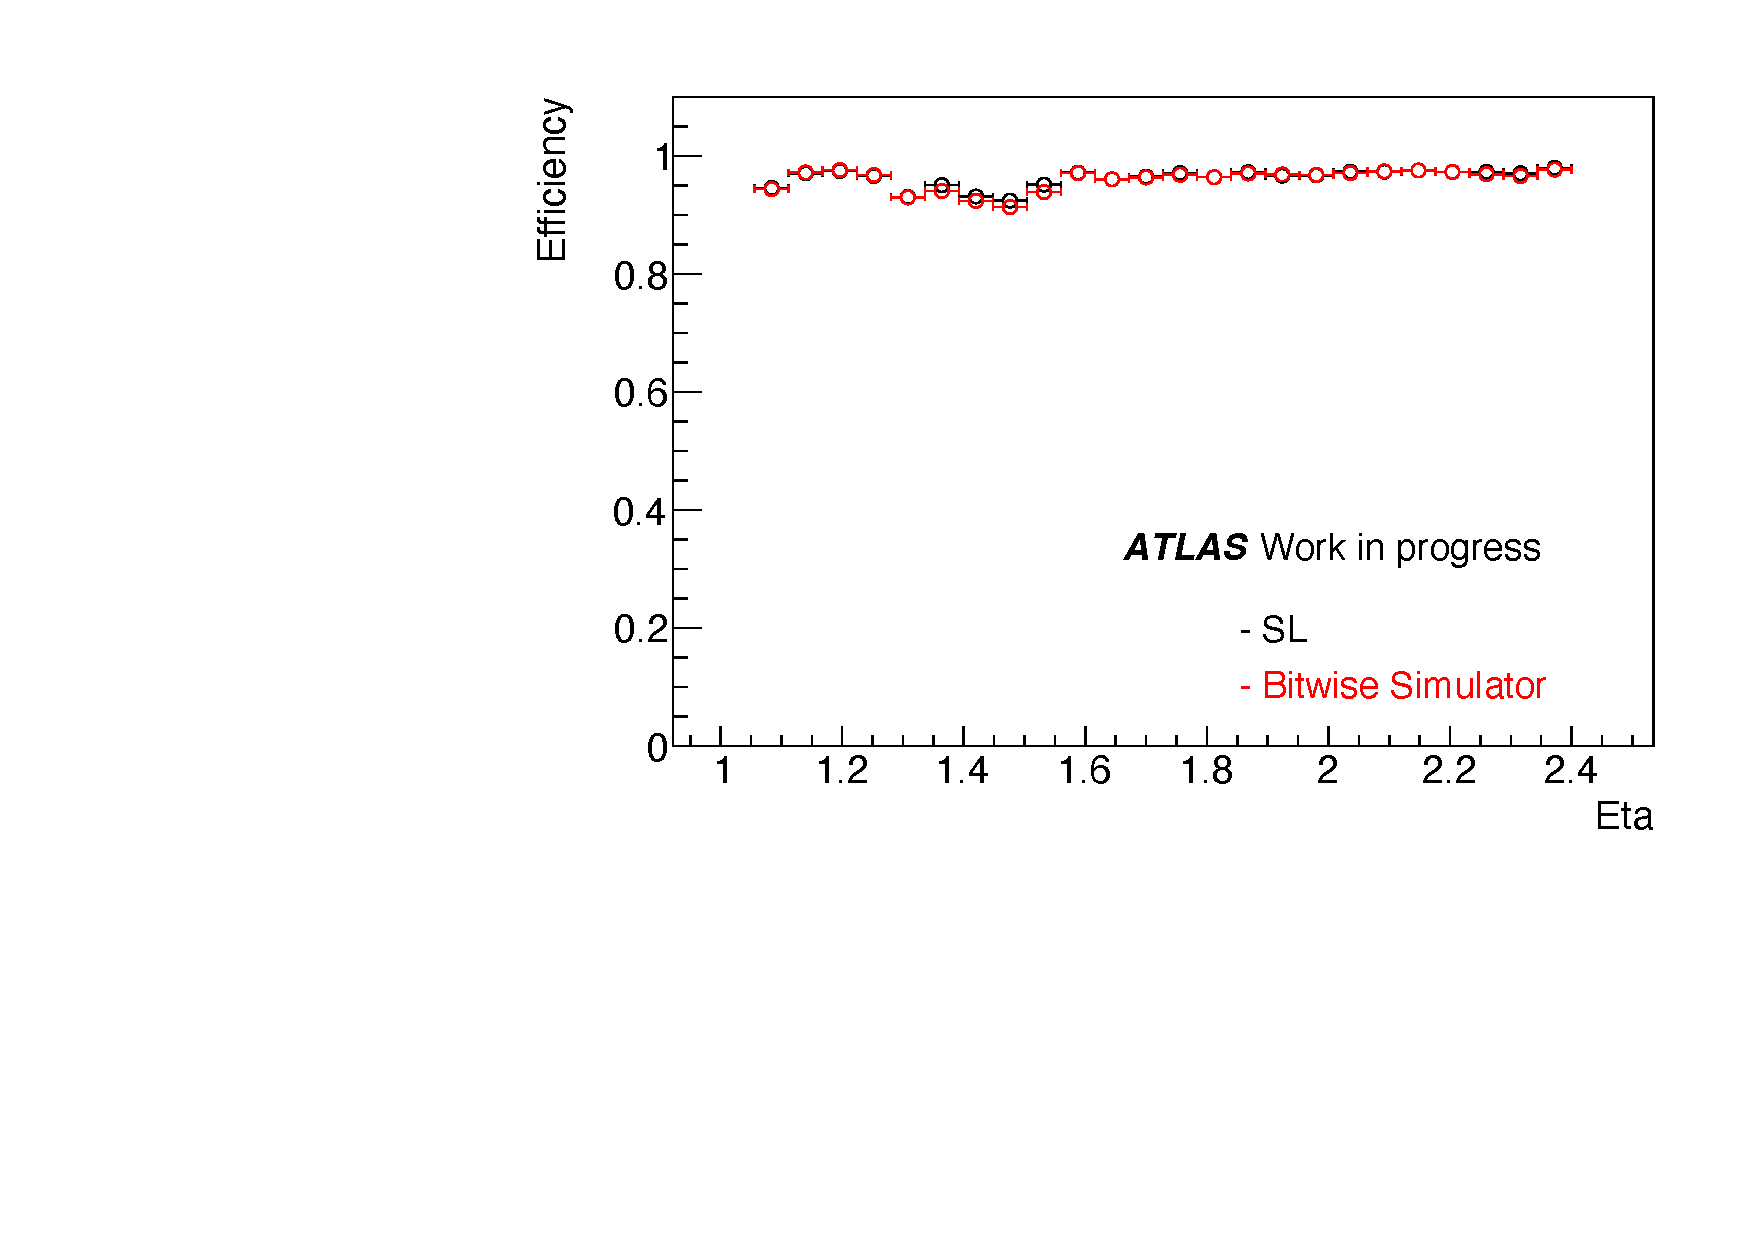
\includegraphics[height=10cm]{fig/Test/A_SM_wire_eta.pdf}
    \subcaption{Wire Segment Reconstructino 検出効率の$\eta$依存性}
    \end{minipage}\\
    \begin{minipage}[b]{\linewidth}
    \centering
    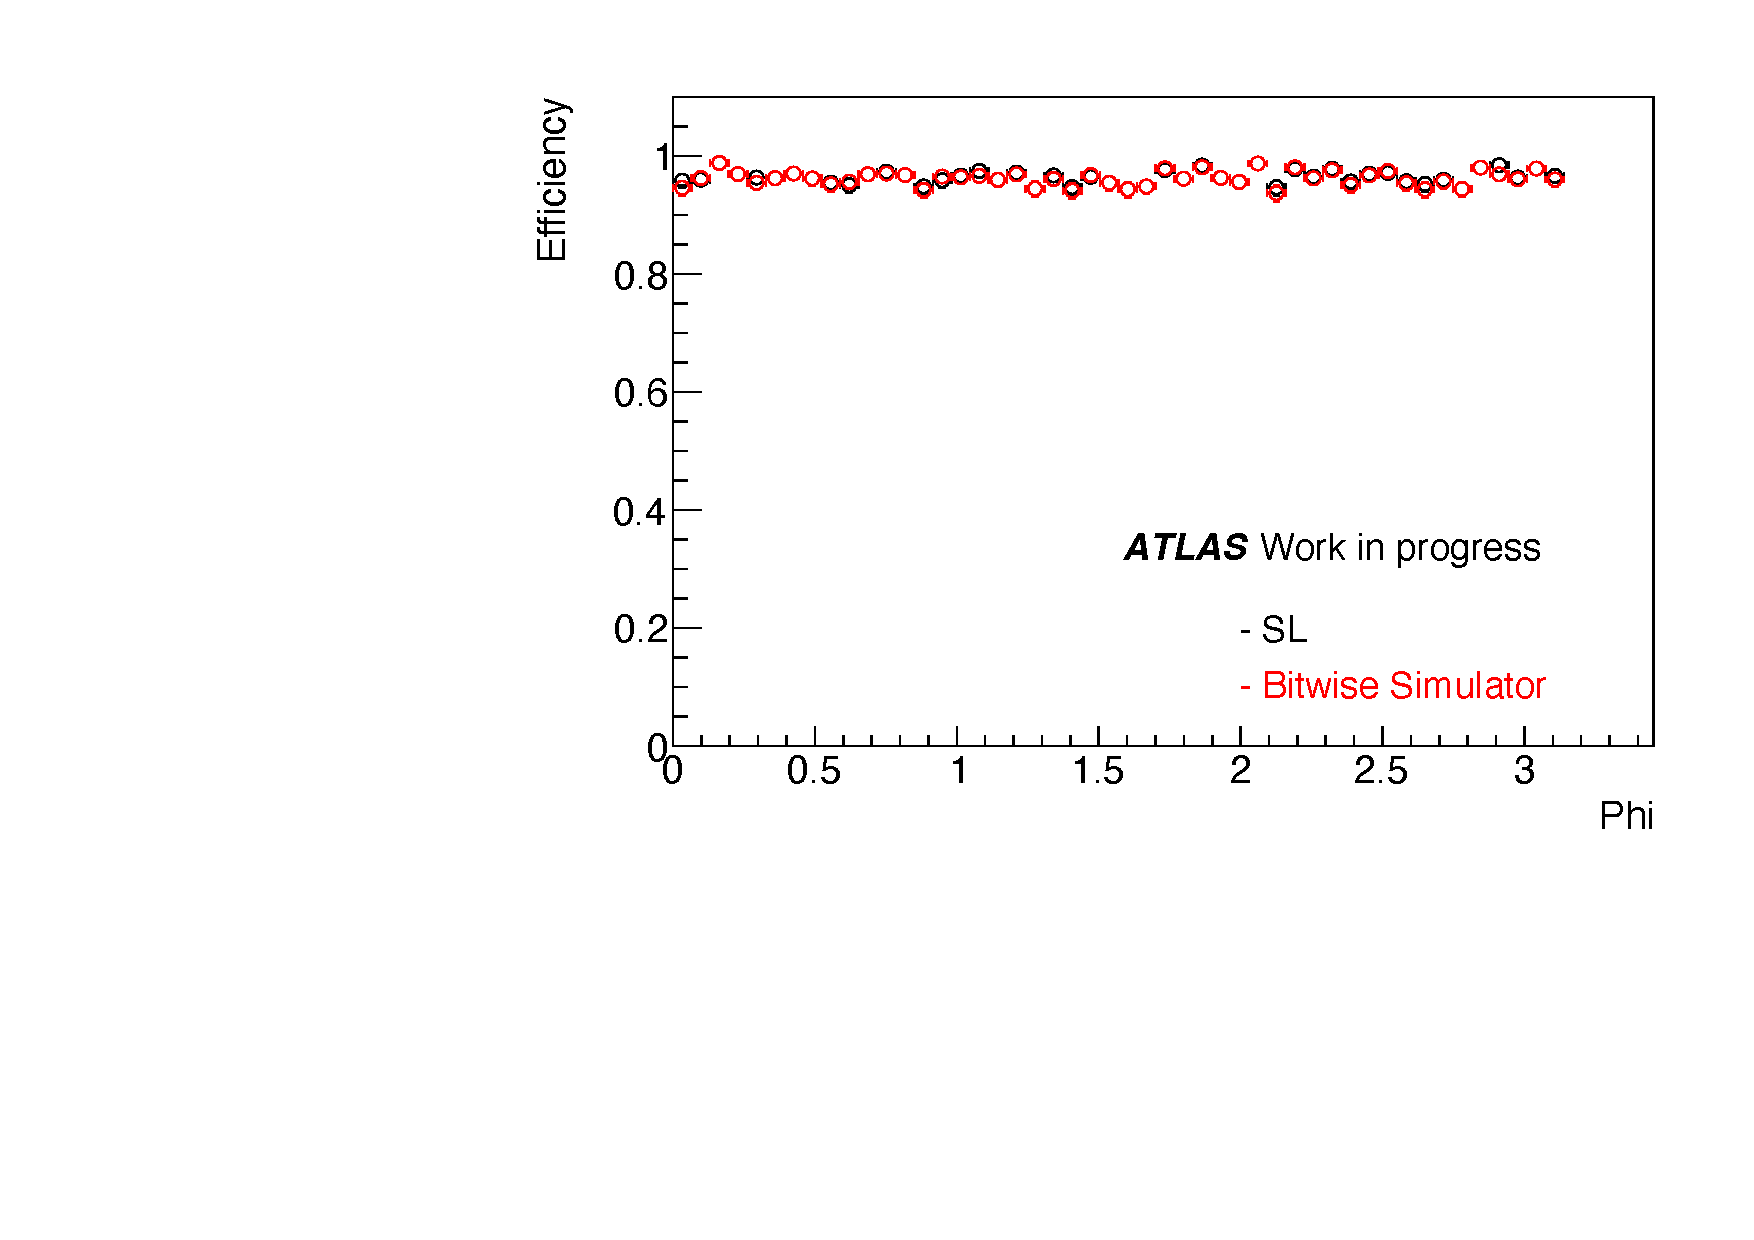
\includegraphics[height=10cm]{fig/Test/A_SM_wire_phi.pdf}
    \subcaption{Wire Segment Reconstructino 検出効率の$\phi$依存性}
    \end{minipage}%
    \caption[Wire Segment Reconstructionの検出効率]{Wire Segment Reconstructionの検出効率。黒色のプロットが実機出力、赤色のプロットがBitwiseシミュレータの出力を表す。全領域のトリガー検出効率は96.3 \%であり、先行研究のソフトウェアシミュレーションやVivadoシミュレーションと矛盾のない結果が得られた。トリガー効率の$\phi$依存性に着目すると、$\eta\sim1.4$付近で5 \%のInefficiencyが見られる。}
    \label{SM_A_Wire}
\end{figure}

\subsubsection{Wire Strip Coincidenceのトリガー効率}
Wire Strip Coincidenceは無限運動量飛跡を用いた試験で既にエンドキャップ領域に不具合が確認されているため、フォワード領域に限定して議論を進める。またStripの試験で明らかになったチェンバー境界領域 ( チェンバーの両端から$\phi$方向に1割の領域 ) の不具合は、Wire Strip CoincidenceのInefficiencyにも直結するため、本試験ではこの領域も除外する。ここではEfficiencyを式\ref{eq:WS_Efficiency}のように定義する。

\begin{equation}
    \mathrm {Efficiency} = \frac{\mathrm{Wire\,Strip\, Coincidenceで\,pt \,閾値\,20\,GeVと判定されたイベント数}}{\mathrm{Truth\,pt \,20 \,GeV以上のイベント数}}
    \label{eq:WS_Efficiency}
\end{equation}

図\ref{SM_A_WS}にWire Strip Coincidenceのフォワード領域検出効率の$\eta$依存性及び$\phi$依存性を示す。平均のトリガー効率は 93.5 \%であり、ソフトウェアシミュレーションの結果と矛盾のない結果が得られた。トリガー効率の$\eta$依存性に着目すると、$\eta\sim1.95、2.2$付近で5 \%のInefficiencyが見られる。この領域は実機の出力とBitwiseシミュレーターの出力で違いが大きく見られる領域でもあるため、BitwiseシミュレーターとVivadoシミュレーターを利用して、まずはこの差の解消に努める。

\begin{figure}
    \begin{minipage}[b]{\linewidth}
    \centering
    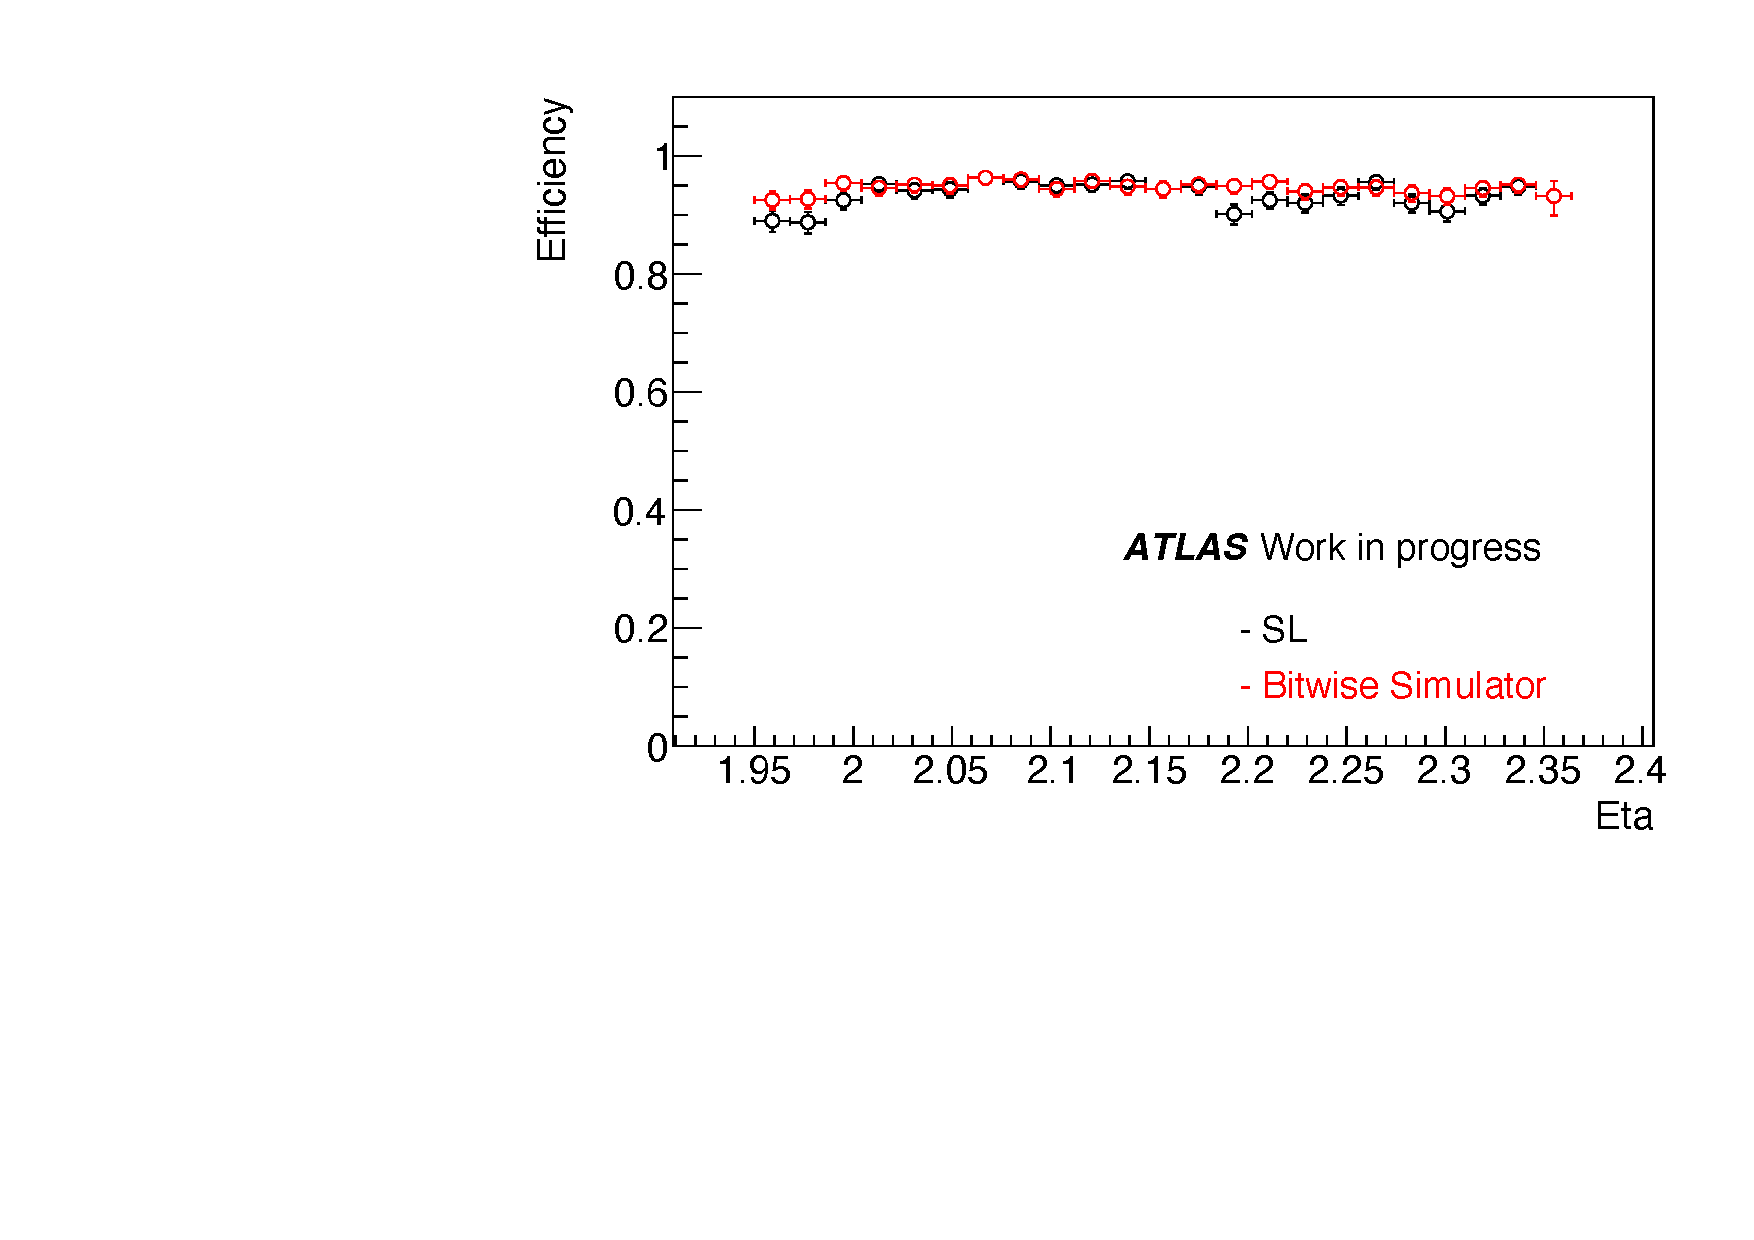
\includegraphics[height=10cm]{fig/Test/A_SM_ws_eta.pdf}
    \subcaption{Wire Strip Coincidence 検出効率の$\eta$依存性}
    \end{minipage}\\
    \begin{minipage}[b]{\linewidth}
    \centering
    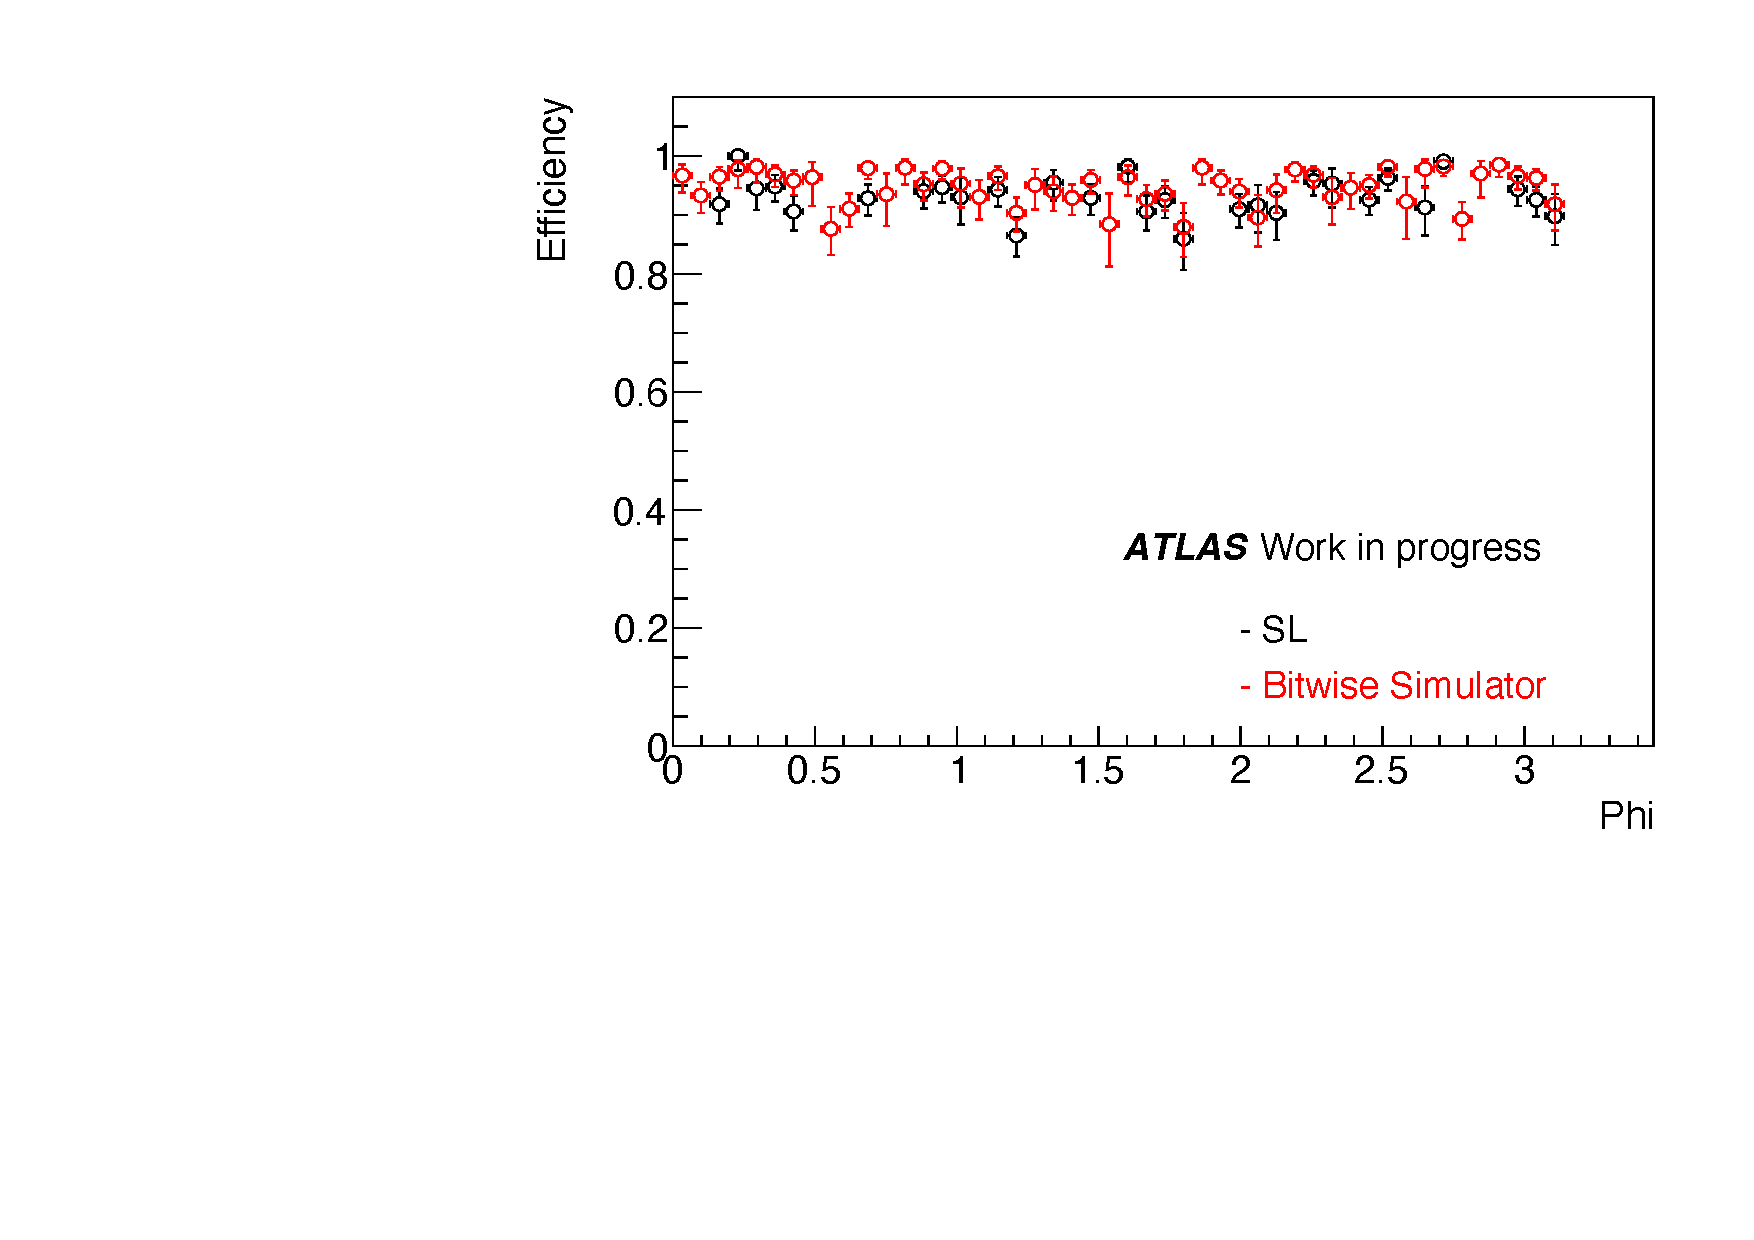
\includegraphics[height=10cm]{fig/Test/A_SM_ws_phi.pdf}
    \subcaption{Wire Strip Coincidence 検出効率の$\phi$依存性}
    \end{minipage}%
    \caption[Wire Strip Coincidenceの検出効率]{フォワード領域におけるWire Strip Coincidenceの検出効率。黒色のプロットが実機出力、赤色のプロットがBitwiseシミュレータの出力を表す。フォワード領域のトリガー検出効率は93.5 \%であり、先行研究のソフトウェアシミュレーションと矛盾のない結果が得られた。トリガー効率の$\eta$依存性に着目すると、$\eta\sim1.95、2.2$付近で5 \%のInefficiencyが見られる。}
    \label{SM_A_WS}
\end{figure}

図\ref{SM_A_WS_turnon}にWire Strip Coincidenceの$p_\mathrm{T}$ごとの検出効率を示す。赤色、青色、緑色、ピンクの各カーブは、それぞれがトリガー閾値20 GeV、15 GeV、10 GeV、5 GeVと判断されたイベントの割合を示しており、一般にこのような図をターンオンカーブという。どの\pt 閾値に対してもプラトー領域のefficiencyは93.5 \%程度であり、ソフトウェアシミュレーションやVivado シミュレーションの結果と一致している (図\ref{Soft_WS})。一方、ソフトウェアシミュレーションの結果と比べて、Efficiencyの立ち上がりが緩やかで、\pt 閾値より小さいイベントを多くトリガーしてしてしまっていることがわかる。例えばWire Segment Reconstructionで不当に$\Delta\eta$を小さく見積もってしまうと、このような振る舞いが生じ得る。今後、ソフトウェアシミュレーターと実機出力でSegment Reconstructionの結果を比較するなどして、原因の解明を行う。

この結果を得るまでに本研究によってWire Segment Reconstructionの問題点が発見され、修正が行われた。詳細をAppendix\ref{sec:appendix:MC-test}に記述する。また、プラトー領域に存在する6.5 \%程度のInefficiencyの原因についてもの調査を行った。この調査結果についてはAppendix\ref{sec:appendix:plateau}に詳細を記述する。
% さらに、今回の試験ではTGC検出器は理想位置と呼ばれる設計段階の位置に設置されていることを仮定して、モンテカルロデータやLUTを作成した。実験本番ではTGC検出器はアライメントの誤差により理想位置からずれた場所に設置される。このずれがトリガー効率にどれほど影響を与えるか調査した。その結果をAppendix{sec:appendix:alignment  \(\)}に示す。

\begin{figure} 
\centering
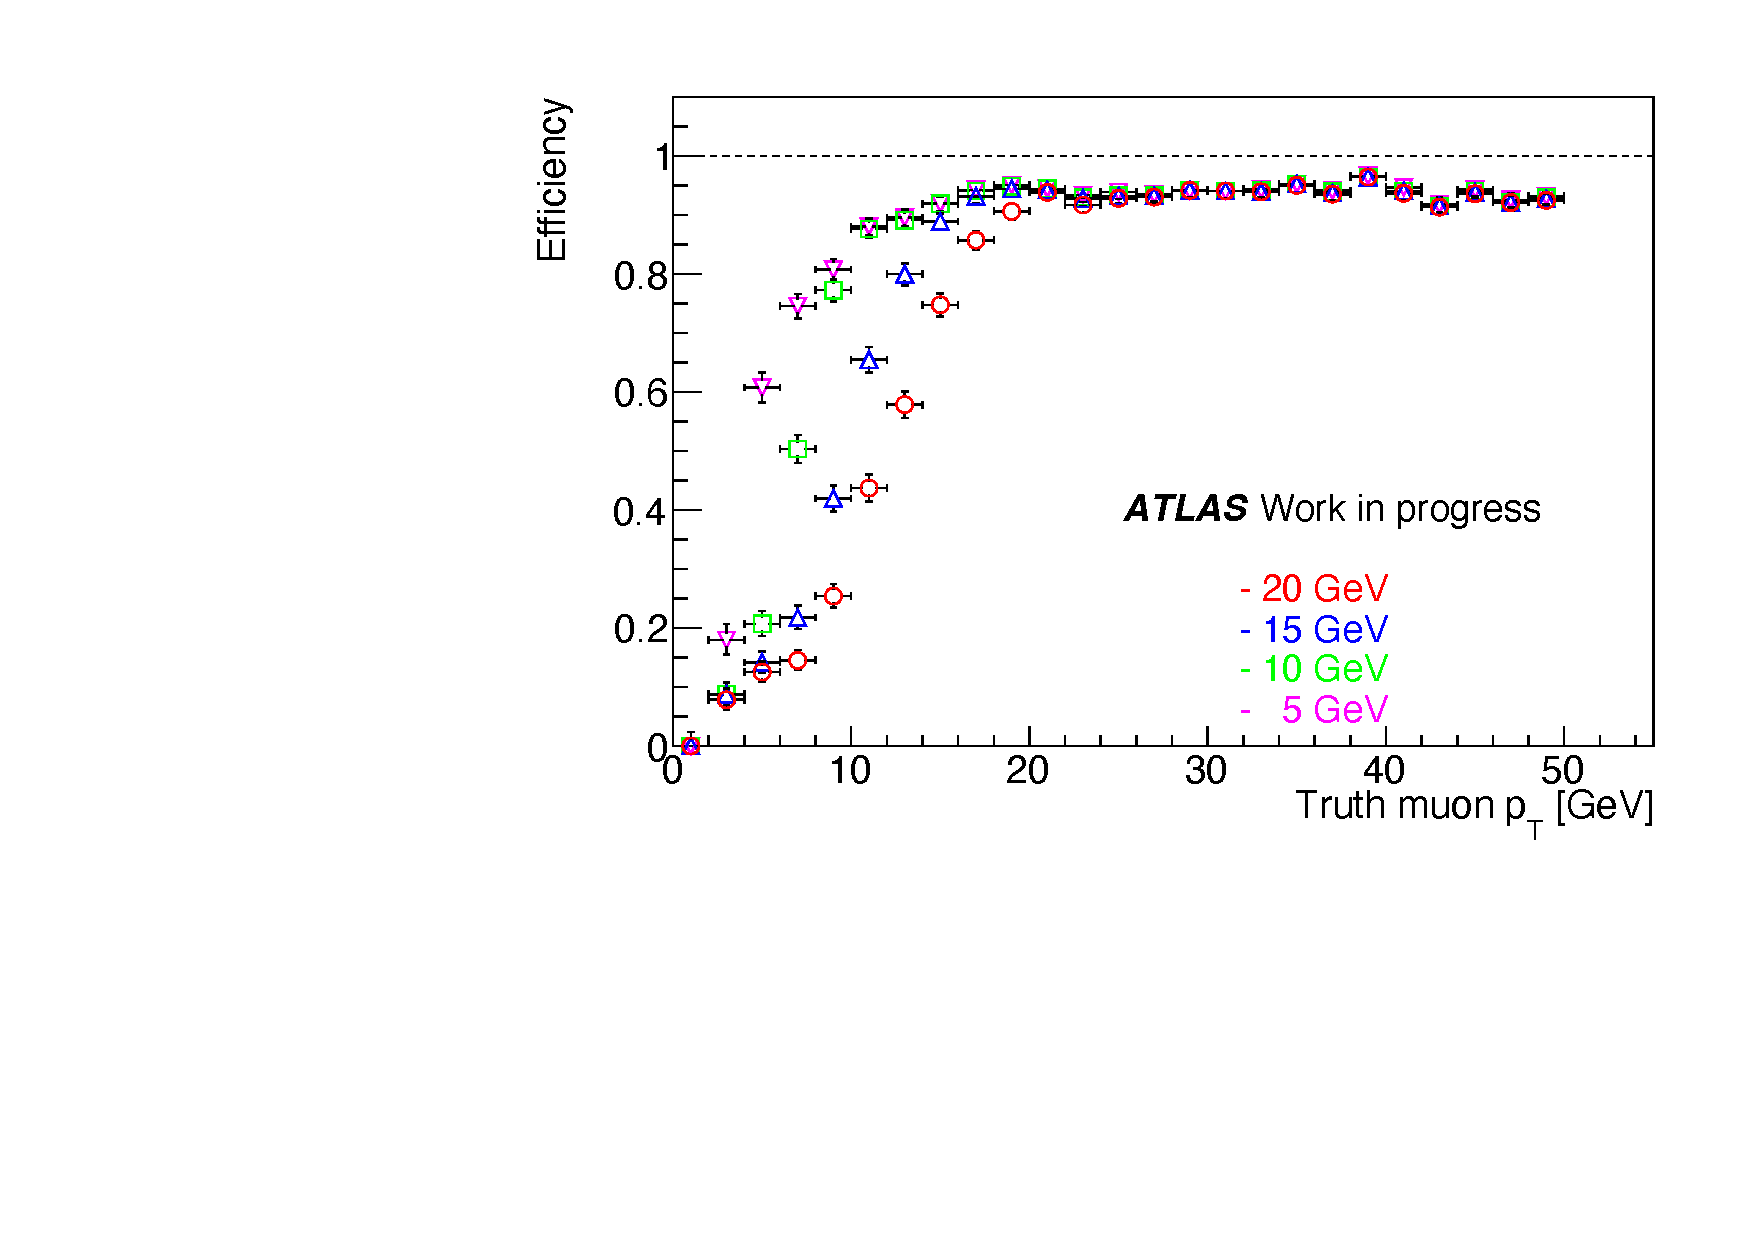
\includegraphics[width=16cm]{fig/Test/A_SM_ws_turn.pdf}   
\caption[]{Wire Strip Coincidenceの$p_\mathrm{T}$ごとの検出効率。赤色、青色、緑色、ピンクの各プロットは、それぞれが $p_{\mathrm{T}}$ 閾値20 GeV、15 GeV、10 GeV、5 GeVと判断されたイベントの割合を示している。プラトー領域のefficiencyはいずれの$p_{\mathrm{T}}$閾値に対しても93.5 \%程度であり、ソフトウェアシミュレーションやVivado シミュレーションの結果と一致している。}
\label{SM_A_WS_turnon}
\end{figure}




